\documentclass[a4paper]{article}
\usepackage[utf8]{inputenc}
\usepackage[T1]{fontenc}

\usepackage[backend=biber,sorting=none]{biblatex}
\addbibresource{references.bib}

\usepackage{amsmath}
\usepackage{appendix}
\usepackage{graphicx}
\usepackage{hyperref}
\usepackage{listings}
\usepackage{placeins}
\usepackage{subcaption}
\usepackage{tabularx}
\usepackage{xcolor}

% \DeclareUnicodeCharacter{03BC}{\textmu}
% \DeclareUnicodeCharacter{B5}{\textmu}

% For fixing unicode errors with lstinputlisting
% https://en.wikibooks.org/wiki/LaTeX/Source_Code_Listings#Encoding_issue
\lstset{literate=
	{µ}{{\textmu}}1
}

\title{PAP328 project work: proportional counter}
\author{Mika Mäki}
\date{2021-04-10}
% TODO add date when the report was handed in

\newenvironment{todo}{
% \hline
\color{red}
}
{
% \hline
}


\begin{document}

\maketitle

\section*{Abstract}
In this project we assembled a gas-based proportional counter for X-ray and $\gamma$-ray detection.
The detector consists of a drink can that serves as the cathode, and a thin anode wire along its center.

% When high voltage is applied between the cathode and the anode and incoming high-energy radiation ionizes the gas inside, the resulting electrons drift towards the anode wire.
% Close to the wire the field strength is high enough for avalanche formation, and the electrons are multiplied, resulting in an electrical pulse that can be detected with read-out electronics.

The system was tested with $^{55}$Fe and $^{241}$Am sources, and a multichannel analyzer was used to collect the emission spectra, which were then analyzed with self-developed software.
The setup was calibrated using the primary $^{55}$Fe and $^{241}$Am X-ray emission peaks, and it demonstrated sufficient resolution  and sensitivity to distinguish two of the the $^{237}$Np L-peaks and one $^{241}$Am peak that belong to the $^{241}$Am decay process.
The voltage dependence of the gas multiplication factor was also investigated.

The detector was also tested with a self-built pre-amplifier.
However, the detector experienced unexpected degradation, due to which the results were inconclusive, but testing the pre-amplifier with another detector was successful.

\tableofcontents


\section{Introduction}
\label{introduction}
Radiation detectors are devices that measure the rate of incoming ionizing radiation such as $\alpha$, $\beta$, $\gamma$ and neutrino radiation and optionally measure its kinetic energies.
They are widely used on various fields from nuclear energy production to medicine.
The properties of ionizing radiation and the needs of applications vary, and so do the detector principles and constructions used.

However, a common feature of particle detectors has been that they are expensive and require various specific tools and materials to manufacture.
In this project work we followed in the footsteps of
\href{https://www.helsinki.fi/en/people/people-finder/alexander-winkler-9110087}{Winkler}
et al. \cite{winkler_gaseous_2015} to demonstrate that proportional counters can be an exception to this by manufacturing a relatively simple proportional counter based on a conventional drink can.
Proportional counters are gas-based radiation detectors, which as their name suggests, produce electric pulses with amplitudes proportional to the energies of the incoming ionizing radiation.
Their operation principles are discussed in section \ref{theory}.

The construction of the proportional counter is discussed in section \ref{assembly}.
To obtain accurate and meaningful results, the system had to be calibrated as in section \ref{assembly} and configured for the measurements as in section \ref{setup_testing}.
The results for the calibration, high voltage sweep and spectral measurements are discussed in section \ref{results}.

We also constructed our own pre-amplifier, but the results were inconclusive due to unexpected degradation of the detector.
These measurements are discussed in the appendix \ref{pre_amp}.


\section{Theory}
\label{theory}

\subsection{Radiation sources and interaction of their radiation with matter}
\iffalse
Radiation can be categorized to ionizing and non-ionizing radiation depending on its capability of exciting electrons out of matter.
In the context of particle physics, the most relevant type of radiation is ionizing radiation, which includes particle radiation and short-wavelength electromagnetic radiation such as X-rays and gamma radiation.
Non-ionizing radiation refers primarily to electromagnetic radiation of visible and longer wavelengths.
In addition to these there are other forms of radiation such as neutrons and neutrinos.
\cite{knoll_radiation_2010}

The effects of electromagnetic radiation vary significantly by wavelength.
Whereas the longer wavelengths are mostly capable of inducing thermal motion, other excitations and electric currents, the shorter wavelengths from ultraviolet radiation onwards have enough energy to remove an electron from an atom or a molecule and are therefore ionizing.
Radiation can also be characterized by its capability of penetrating matter, which is called the hardness of the radiation.
Generally the hardness increases with the energy of the quanta.
\cite{knoll_radiation_2010}

Alpha and beta radiation are the most prominent types of particle radiation.
Alpha radiation consists of 
\fi

In the context of particle physics, the most relevant type of radiation is ionizing radiation, which includes particle radiation and short-wavelength electromagnetic radiation such as X-rays and gamma radiation.
In this project $^{55}$Fe and $^{241}$Am sources were used.
$^{55}$Fe decays by electron capture of the innermost shell (K-shell) into $^{55}$Mn with a half-life of 2.75 a.
This results in an electron vacancy, which gets filled by an electron from the outer shells, resulting in a sequence of electron transfers, the energy of which is released as Auger electrons and soft X-ray emissions.
$^{241}$Am decays by $\alpha$-decay to $^{237}$Np with the reaction
\begin{equation}
^{241}_{95}\text{Am} \rightarrow ^{237}_{93}\text{Np} + ^4_2 \alpha + \gamma (59.24 \text{keV}),
\end{equation}
therefore producing a weak $\gamma$-ray as a byproduct.
However, due to the closed packaging of the sources, only the X- and $\gamma$-rays were allowed to escape the sources.
\cite{winkler_gaseous_2015}

There are three primary mechanisms for the interaction of X- and $\gamma$-rays with matter.
These are photoelectric absorption, Compton scattering and pair production.
In photoelectric absorption the photon is completely absorbed by an atom, and its energy is transferred to an electron that gets excited out of the atom, resulting in ionization and a vacancy in the shell.
With high-energy $\gamma$-rays the excited electrons are usually from the innermost shells such as the K-shell.
These vacancies get quickly filled by electrons from the outer shells, and the excess energy is released by characteristic X-rays and Auger electrons.

Compton scattering is the predominant mechanism for the $\gamma$-rays of radioisotope sources.
In Compton scattering the photon is deflected by an electron of the absorbing material, and some of the kinetic energy of the photon gets transferred to the electron, resulting in ionization.

If the $\gamma$-ray energy exceeds twice the rest-mass of an electron (1.02 MeV), the $\gamma$-ray may get
However, the energies in 



These interactions and the interactions of particle radiation with matter are discussed with more detail in the book \textit{Radiation Detection and Measurement} \cite{knoll_radiation_2010}.




\subsection{The proportional counter}
\label{counter}

In this project the particle detection was done using a proportional counter, which is a gas-filled particle detector with a high electric field inside.
\cite{instructions}
A schematic of the proportional counter is given in figure \ref{fig:theory_schematic}.

\begin{figure}[ht!]
\centering
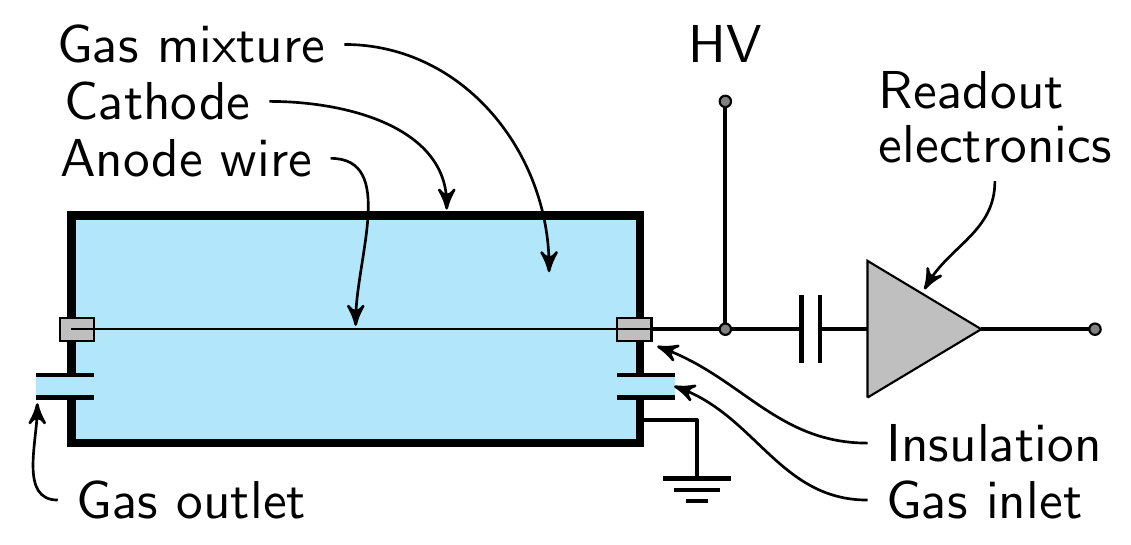
\includegraphics[width=0.6\textwidth]{fig/article/schematic.png}
\caption{Schematic drawing of the proportional counter \cite{winkler_gaseous_2015}}
% TODO: draw own version with vector graphics
\label{fig:theory_schematic}
\end{figure}

When ionizing radiation passes through the detector, it collides with the gas inside, causing ionization of the gas.
Due to the electric field the electrons drift towards the anode, and the positive ions drift towards the cathode.
This causes a pulse of electric current, which is detectable with the readout electronics.
The detector is cylindrically symmetric, and the electric field strength can therefore be approximated as
\begin{equation}
E(r) = \frac{U}{r \ln(b/a) },
\end{equation}
where $U$ is the potential between the electrodes, $r$ is the radius of the can, $a$ is the outer radius of the anode wire and $b$ is the inner radius of the cathode tube.
Consequently, the electric field strength increases when approaching the anode wire, and close to the anode ($\approx$ 30 \textmu m) it reaches sufficient level for
\href{https://en.wikipedia.org/wiki/Townsend_discharge}{Townsend avalanche} formation.
In a Townsend avalanche the kinetic energy of a drifting electron is sufficient to ionize the gas upon collisions, and this results in the multiplication of the incomng electron.
As the naming of the proportional counter suggests, the number of generated electron-ion pairs is proportional to those generated by the incident radiation, and consequently incoming particles of different energies can be distinquished to create spectral measurements.
\cites{winkler_gaseous_2015}[p. 159--164]{knoll_radiation_2010}

The uniformity of the detector and especially the anode wire is highly important for the spectral accuracy of the detector.
However, in the ends of the detector this is not achieved, as the field distortion caused by the shape of the detector is significant.
As a solution the anode wire at the ends is covered by metallic field tubes, which increase the radius of the anode and consequently prevent the formation of avalanches in those regions.
\cite[p. 165]{knoll_radiation_2010}

Each avalanche creates a cloud of positive ions near the anode, and these slowly diffuse towards the cathode.
The anode wire is long compared to the avalanche, and therefore the detector can record other pulses from other regions of the wire before the ions have cleared from the first one.
However, the applied voltage and consequently the electric field is too high, the avalanches become so large that the ions form a significant space charge in the detector, which alters its characteristics and causes nonlinearities in its behaviour.
This is known as the limited proportionality region.
If the applied voltage is increased further, the space charge becomes a dominant feature.
It reduces the field near the anode and therefore limits the avalanche process, causing all pulses to have the same amplitude.
This is known as the Geiger-Mueller region.
\cite[p. 160--161]{knoll_radiation_2010}

The choice of the gas mixture is essential for the operation of the detector.
The operation of a proportional counter is dependent on the migration of free electrons, which should not be absorbed during their journey.
The gas should therefore have a low electron attachment coefficient.
This disqualifies the use of air, and the detectors should consequently be airtight to prevent the introduction of air into the detector chamber.
\cite[p. 167--168]{knoll_radiation_2010}

The avalanche collisions near the anode wire may cause excitations of the gas in addition to the desired ionization.
These excitations decay by the emission of visible or UV photons, which can cause ionization elsewhere in the detector under suitable circumstances.
These would lead to a loss of proportionality or the creation of spurious pulses, which are undesirable in proportional counters.
To alleviate this problem, a molecular gas is introduced into the mixture to absorb these photons.
In this project we used the P-10 gas mixture, which consists of 90 \% argon and 10 \% methane.
\cite[p. 168]{knoll_radiation_2010}


Gas constants \cite{wolff_measurement_1974}

Theoretical predictions on accuracy?

Schockley \cite{shockley_currents_1938}
Ramo \cite{ramo_currents_1939}
TODO

Diethorn formula \cite[eq. 6.10]{knoll_radiation_2010}
\begin{equation}
\ln M = \frac{V}{\ln b/a} \frac{\ln 2}{\Delta V}
\left( \ln \frac{V}{pa \ln (b/a)} - \ln K \right)
\end{equation}


\subsection{Error analysis methods}
\label{error_analysis}
The detector consists of various components, each of which has its manufacturing imperfections.
In addition, each of the measurement systems used has inaccuracies.
Together these provide various sources of uncertainties for the measurements, and combining these into uncertainties of the end results is known as error propagation.

By Taylor expanding the function in question around the mean values of the random variables we can relate the covariance matrices and therefore the uncertainties of the input and output variables.
In the general case the covariance matrix of the output variables is given by
\begin{equation}
U_{kl}
= \mathrm{Cov}(y_k, y_l)
\approx \sum_{i,j=1}^n \left( \frac{\partial y_k}{\partial x_i} \frac{\partial y_l}{\partial x_j} \right)_{\mathbf{x}=\mathbf{\mu}} V_{ij},
\end{equation}
where $U$ is the covariance matrix of the output variables $y$ and $V$ is the covariance matrix of the input variables $x$.
Consequently the variances for each of the output variables are
\begin{equation}
\sigma_{y_k}^2 \approx \sum_{i,j=1}^n \left( \frac{\partial y_k}{\partial x_i} \frac{\partial y_k}{\partial x_j} \right)_{\mathbf{x}=\mathbf{\mu}} V_{ij}.
\end{equation}
This can be written in matrix notation as
\begin{equation}
U = AVA^T,
\end{equation}
where
\begin{equation}
A_{ij} = \frac{\partial y_i}{\partial x_j} \vert_{\boldsymbol{x}=\boldsymbol{\mu}}.
\end{equation}
\cite[p. 20--22]{cowan_statistical_1998}

If the input variables $x_i$ are uncorrelated, these expressions are simplified.
Then the covariance matrix is given by
\begin{equation}
U_{kl} \approx \sum_{i=1}^n \left( \frac{\partial y_k}{\partial x_i} \frac{\partial y_l}{\partial x_i} \right)_{\mathbf{x}=\mathbf{\mu}} \sigma_i^2,
\end{equation}
and the variances are \cite[p. 20--22]{cowan_statistical_1998}
\begin{equation}
\sigma_{y_k}^2 \approx \sum_{i=1}^n \left( \frac{\partial y_k}{\partial x_i} \right)_{\mathbf{x}=\mathbf{\mu}}^2 \sigma_i^2.
\label{eq:variance}
\end{equation}
In the analysis code of this project the general case of this error propagation has been implemented using
\href{https://www.sympy.org/}{SymPy},
which calculates the necessary partial derivatives symbolically.
This is used for the computation of the collected charges and the Diethorn formula.
The error propagation of fit functions is handled directly by the
\href{https://docs.scipy.org/doc/scipy/reference/generated/scipy.optimize.curve_fit.html}{scipy.optimize.curve\_fit}
and
\href{https://docs.scipy.org/doc/scipy/reference/generated/scipy.odr.ODR.html}{scipy.odr.ODR} utilities of
\href{https://www.scipy.org/}{SciPy}
that are used to generate the fits.
\cite{repo}


\iffalse
\subsection{Error analysis}
\begin{todo}
The total gain of the amplifiers is a product of the gains of the pre-amplifier and the spectral amplifier.
Therefore the uncertainty of the gain using equation \ref{eq:variance} is
\begin{equation}
\sigma_g \approx \sqrt{(g_\text{spec} \sigma_\text{pre})^2 + (g_\text{pre}\sigma_\text{spec})^2}.
\end{equation}
TODO: the gain of the spectral amplifier was varied from $10\cdot1=10$ to $10\cdot100=1000$, but what was the gain of the pre-amplifier?
Since they were two parts of the same device, was the setting already a total of these?
Was the coarse gain perhaps for the pre-amplifier and the fine gain for the spectral amplifier?
\end{todo}
\fi


\iffalse
\subsection{Read-out electronics}
\label{electronics}


Capacitive decoupling \ref{fig:theory_schematic}

The detector was also tested with a custom pre-amplifier, and the results are in appendix \ref{pre_amp}.
\fi


\clearpage
\section{Experimental set-up}
\label{setup}
As a part of this project we built the detector ourselves from a construction kit designed by the course organizers.
For the read-out electronics we used devices available in the laboratory.

Answer the questions on page 5 of the instructions!


\subsection{Detector assembly}
\label{assembly}
The detector of this project was manufactured from an aluminum drink can according to the schematic of figure \ref{fig:schematic}.
The parts were provided by the course organizers, except for the drink can.

\begin{figure}[ht!]
\centering
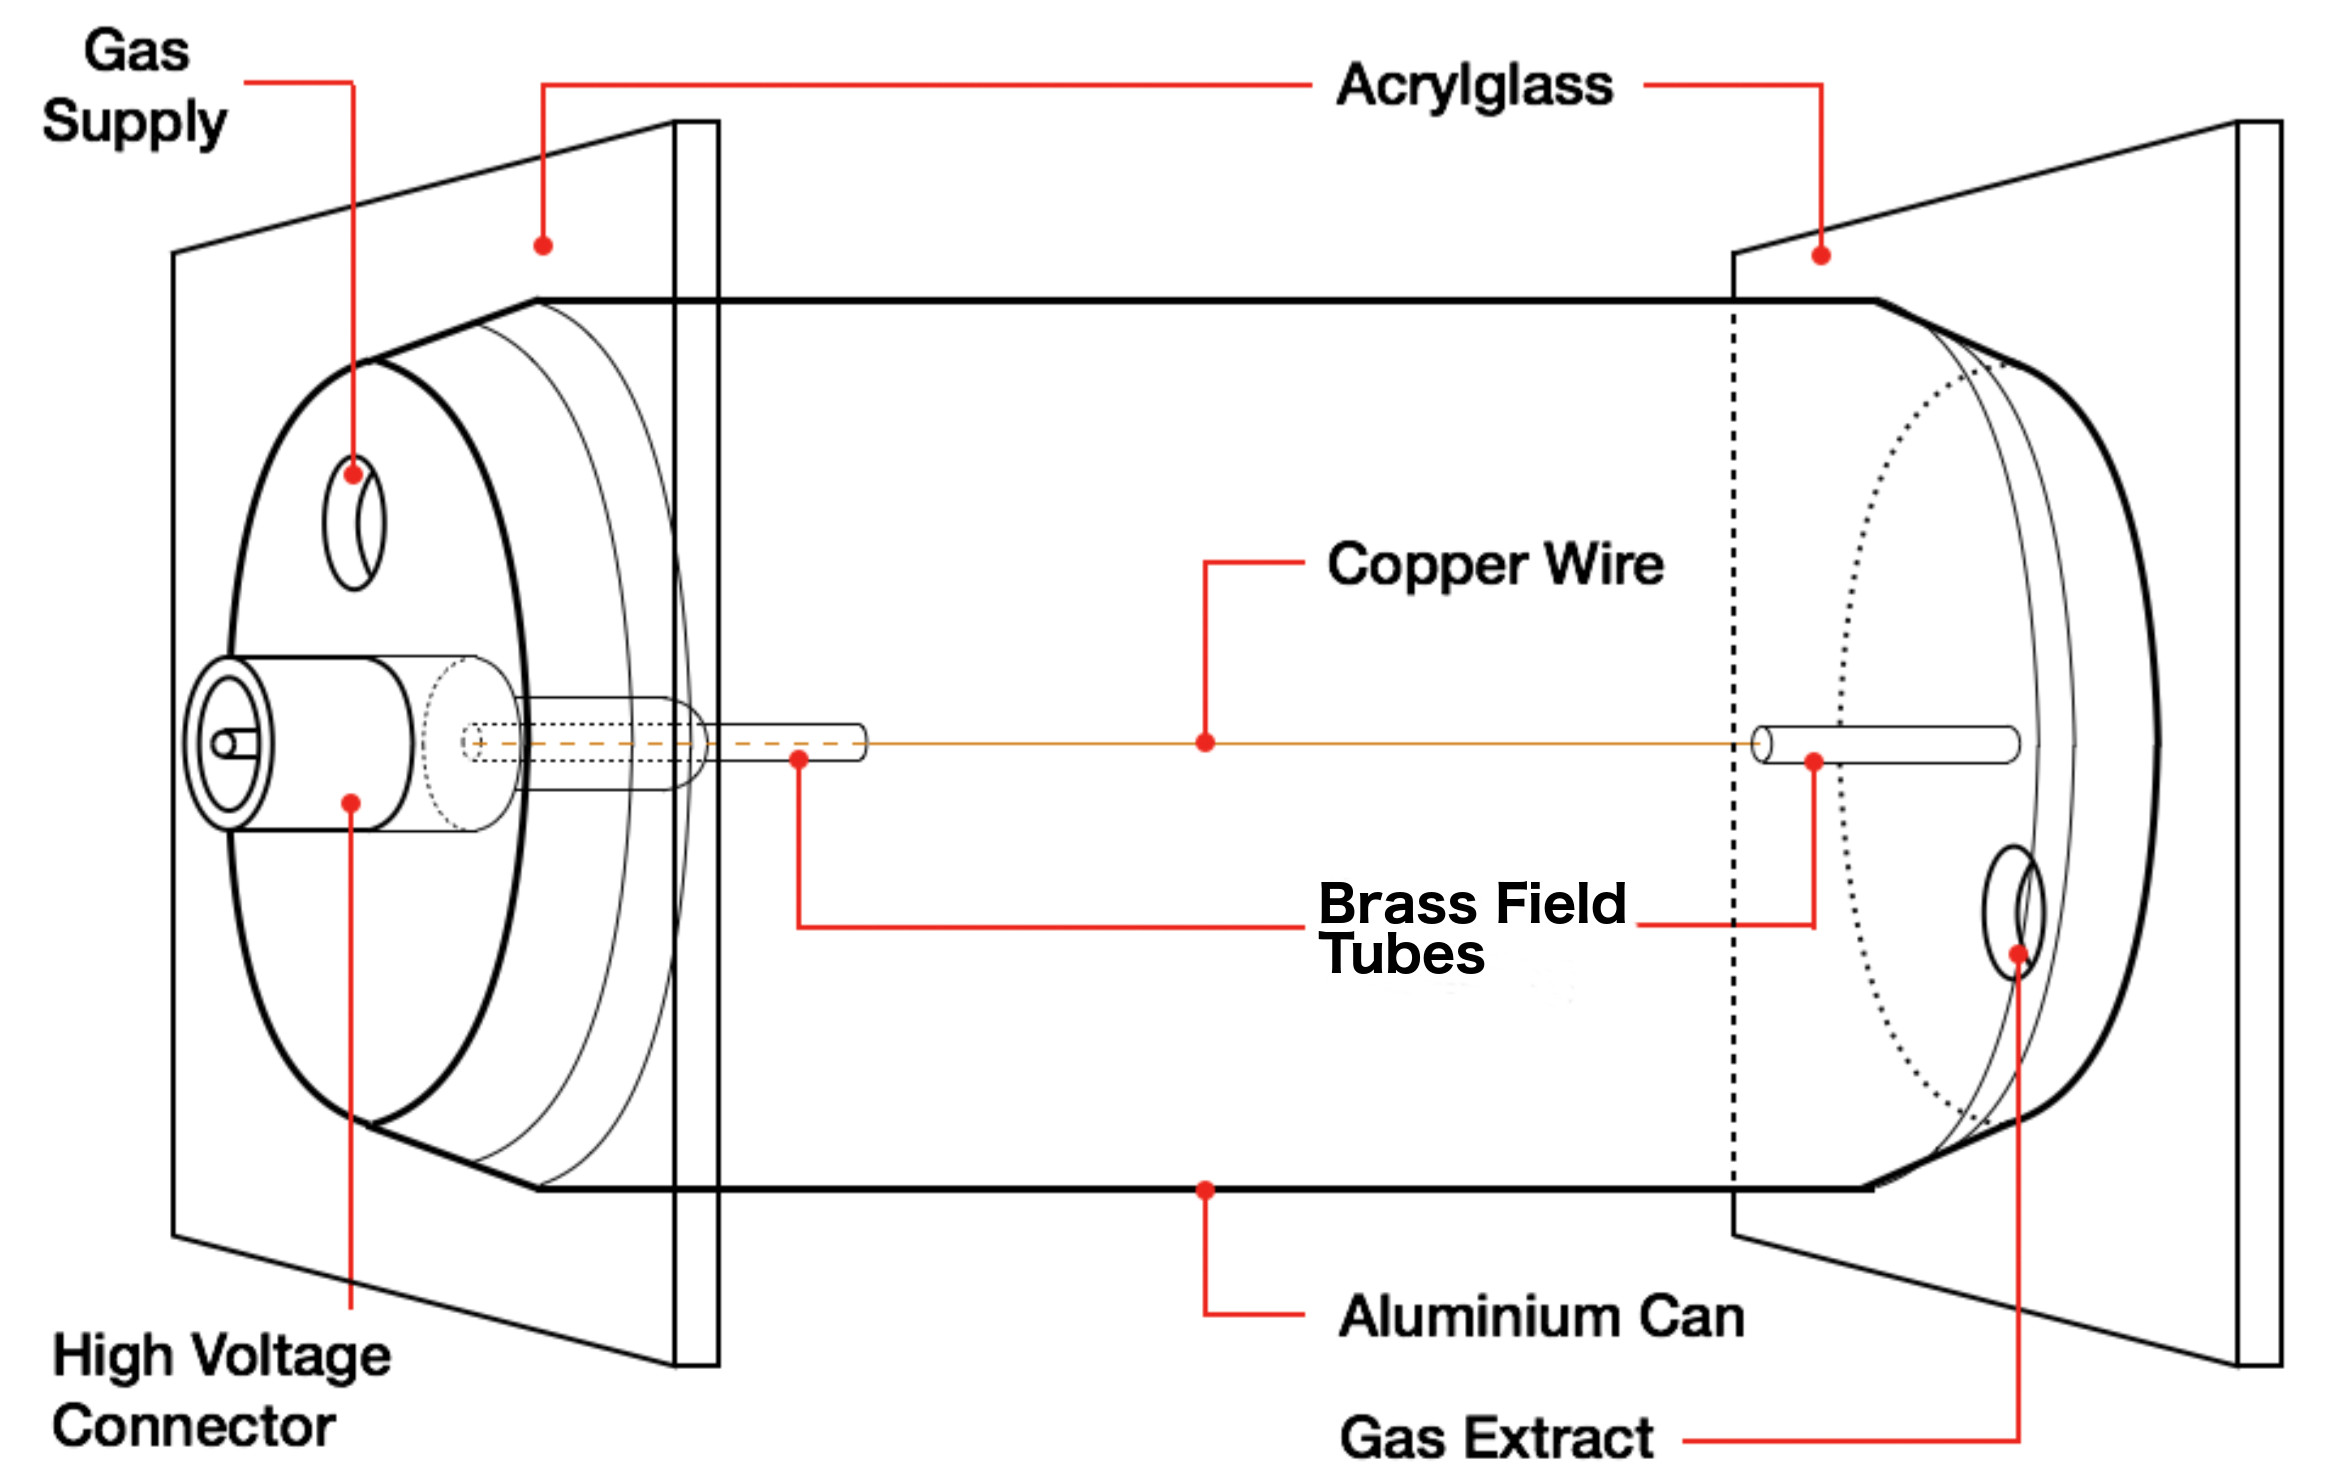
\includegraphics[width=0.8\textwidth]{fig/instructions/schematic.png}
\caption{Schematic of the detector \cite{instructions}}
% TODO draw own one with vector graphics
\label{fig:schematic}
\end{figure}

First the parts were prepared by removing a single strand from a copper wire and cutting two pieces of brass tube for the wire mounting.
The course organizers removed the top of the can and drilled two holes to its bottom, one to the center and one off-center.
The cutting edges were then smoothened to avoid sharp edges that could cause sparking, and the anti-corrosion layer was grinded away for long-term stability of the detector.
Table \ref{table:sizes} contains size measurements of the can and the brass tubes.
Each of the results is averaged from five measurements.
The can thickness and brass tube diameter were measured using a
\href{https://en.wikipedia.org/wiki/Micrometer}{micrometer}, and the rest were measured with a
\href{https://en.wikipedia.org/wiki/Calipers}{caliper}.

Once the can and the other parts were ready, they were put to an ultrasonic cleaner for grease removal, as any leftover grease in the detector could interact due to the high-voltage conditions, causing degradation of detector performance.
To avoid contaminating the cleaned parts, every step from now on had to performed with rubber gloves.

The anode mounting was prepared by gluing the longer brass tube to the hole in the center of a plastic screw.
To avoid filling the hole within the brass tube, the outside of the brass tube was coated with glue, and the tube was then pushed into the hole.
The screw was then attached to the can with a plastic nut, as in figure \ref{fig:anode_mounting}.

\begin{figure}[ht!]
\centering
\begin{subfigure}[t]{0.48\textwidth}
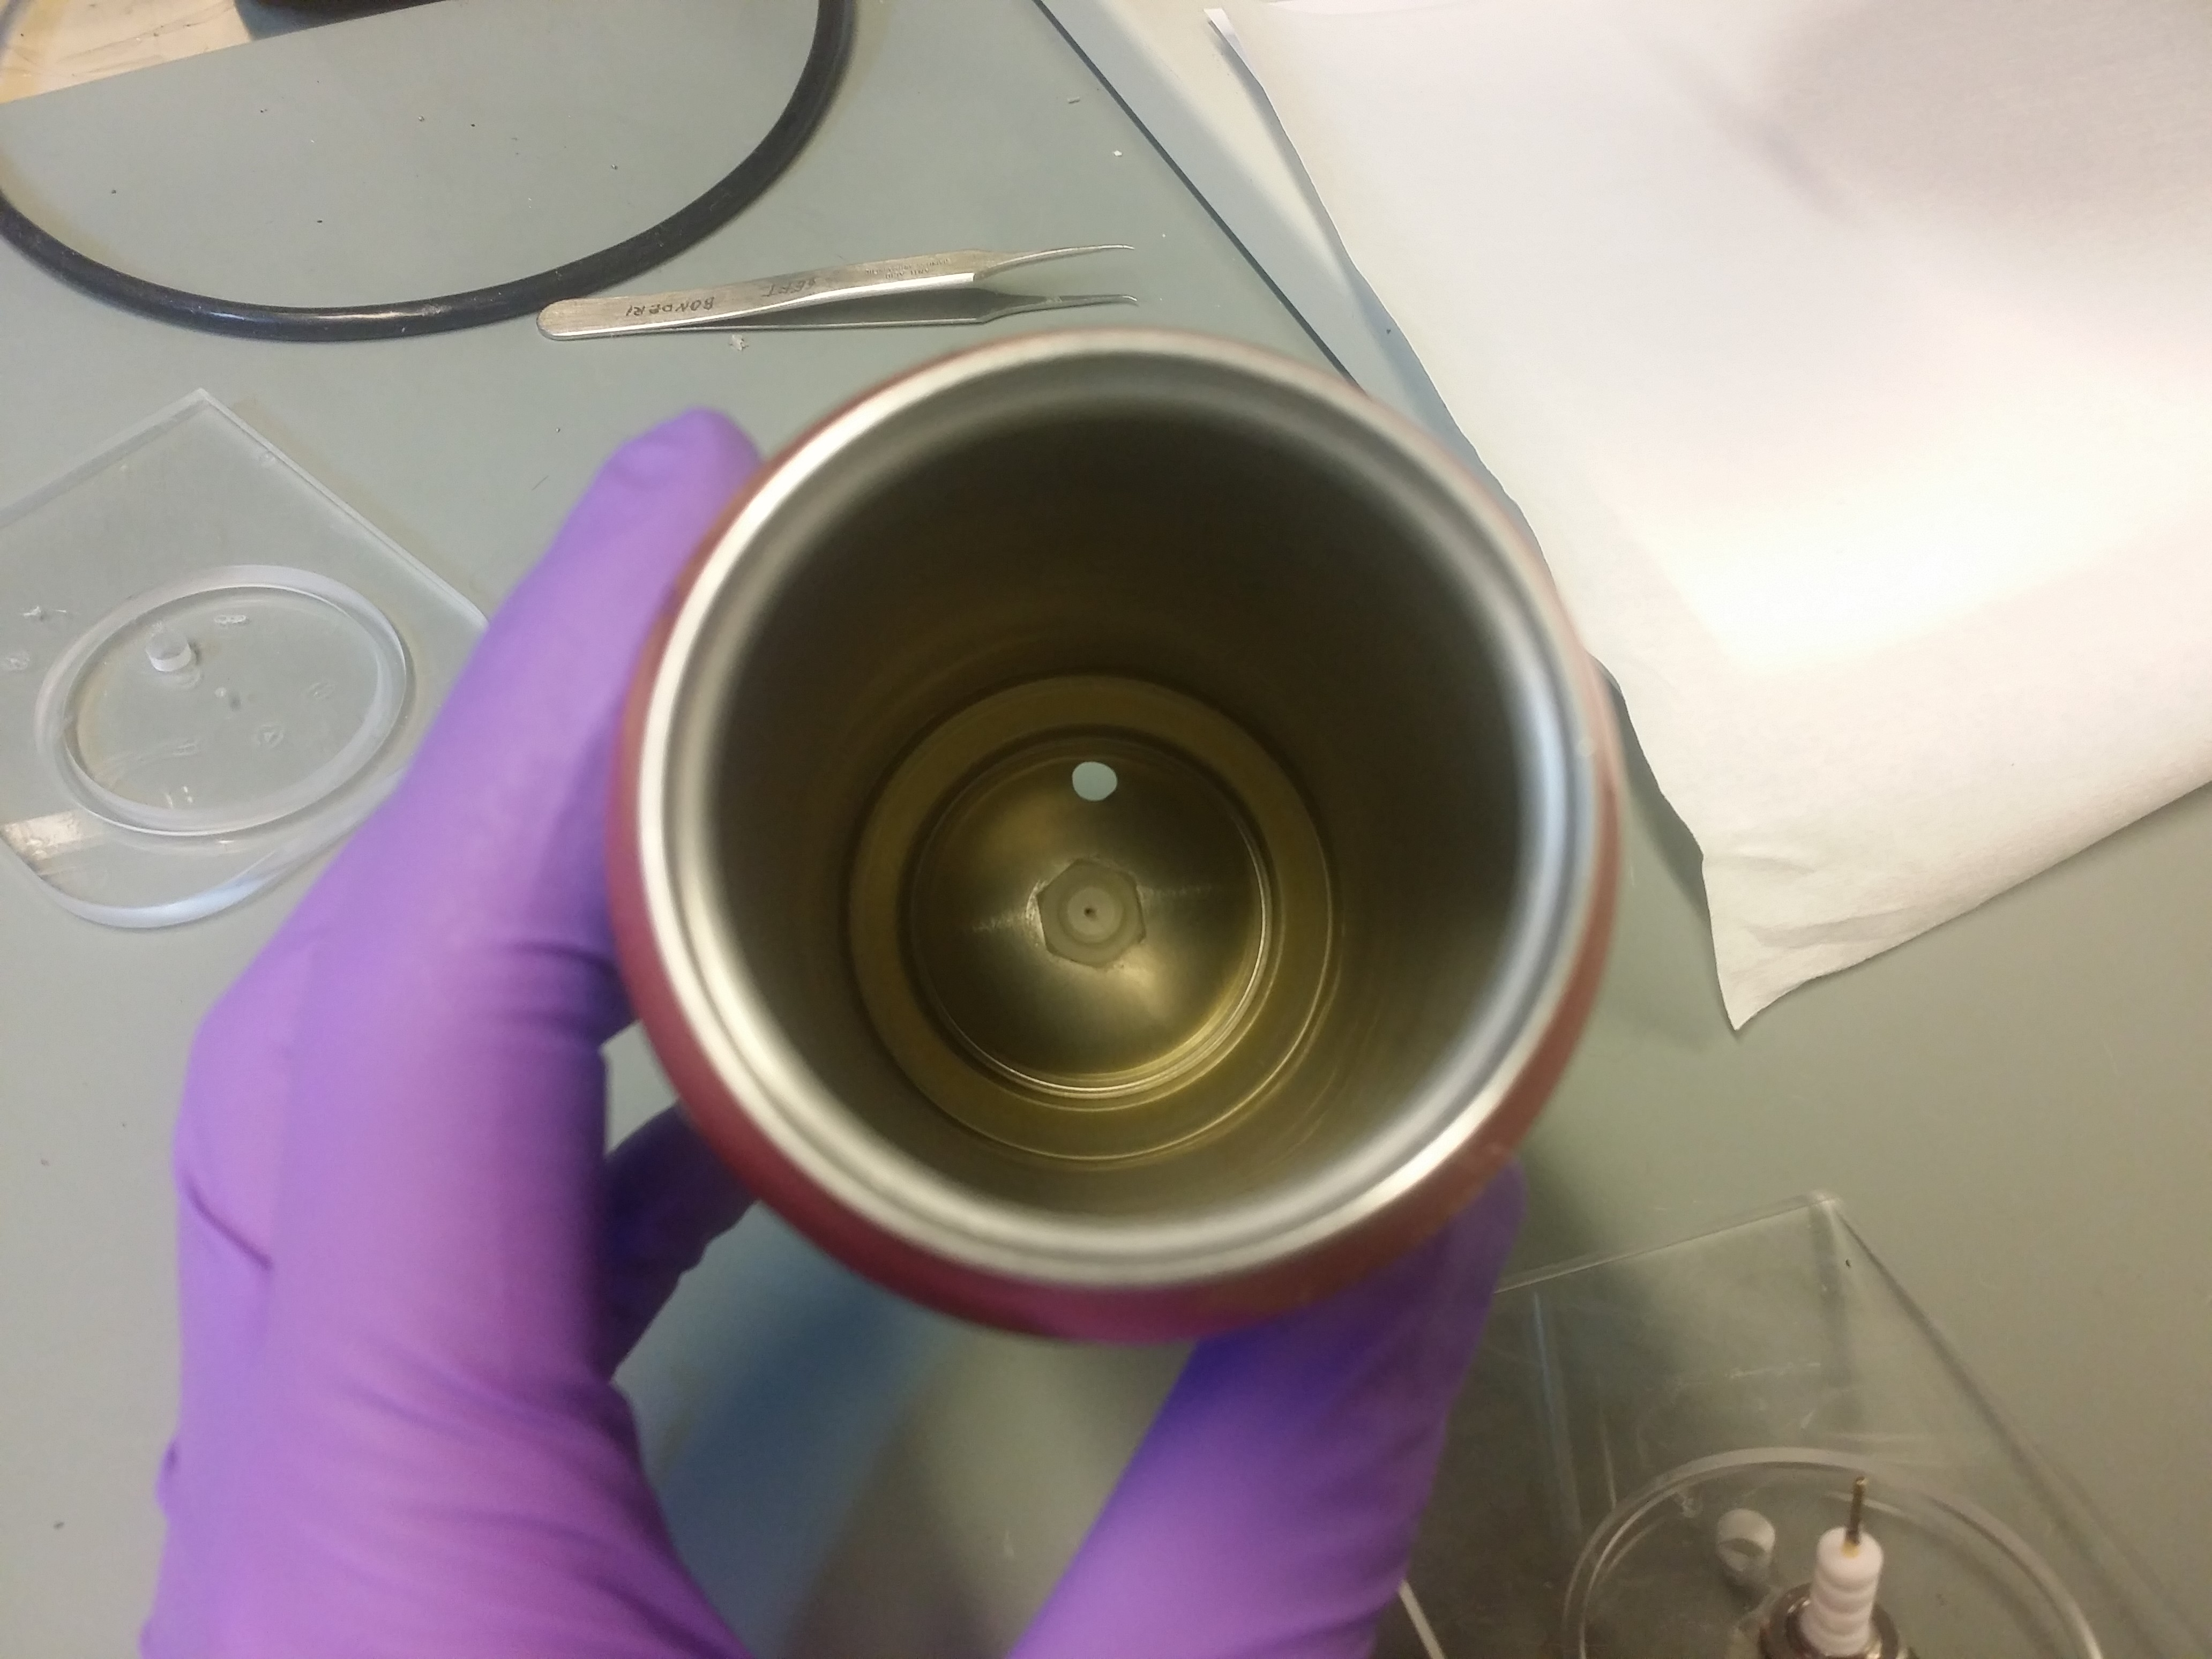
\includegraphics[width=\textwidth]{fig/IMG_20201123_103327.jpg}
\caption{A brass tube within a plastic screw serves as the other end of the anode wire}
\label{fig:anode_mounting}
\end{subfigure}
%
\begin{subfigure}[t]{0.48\textwidth}
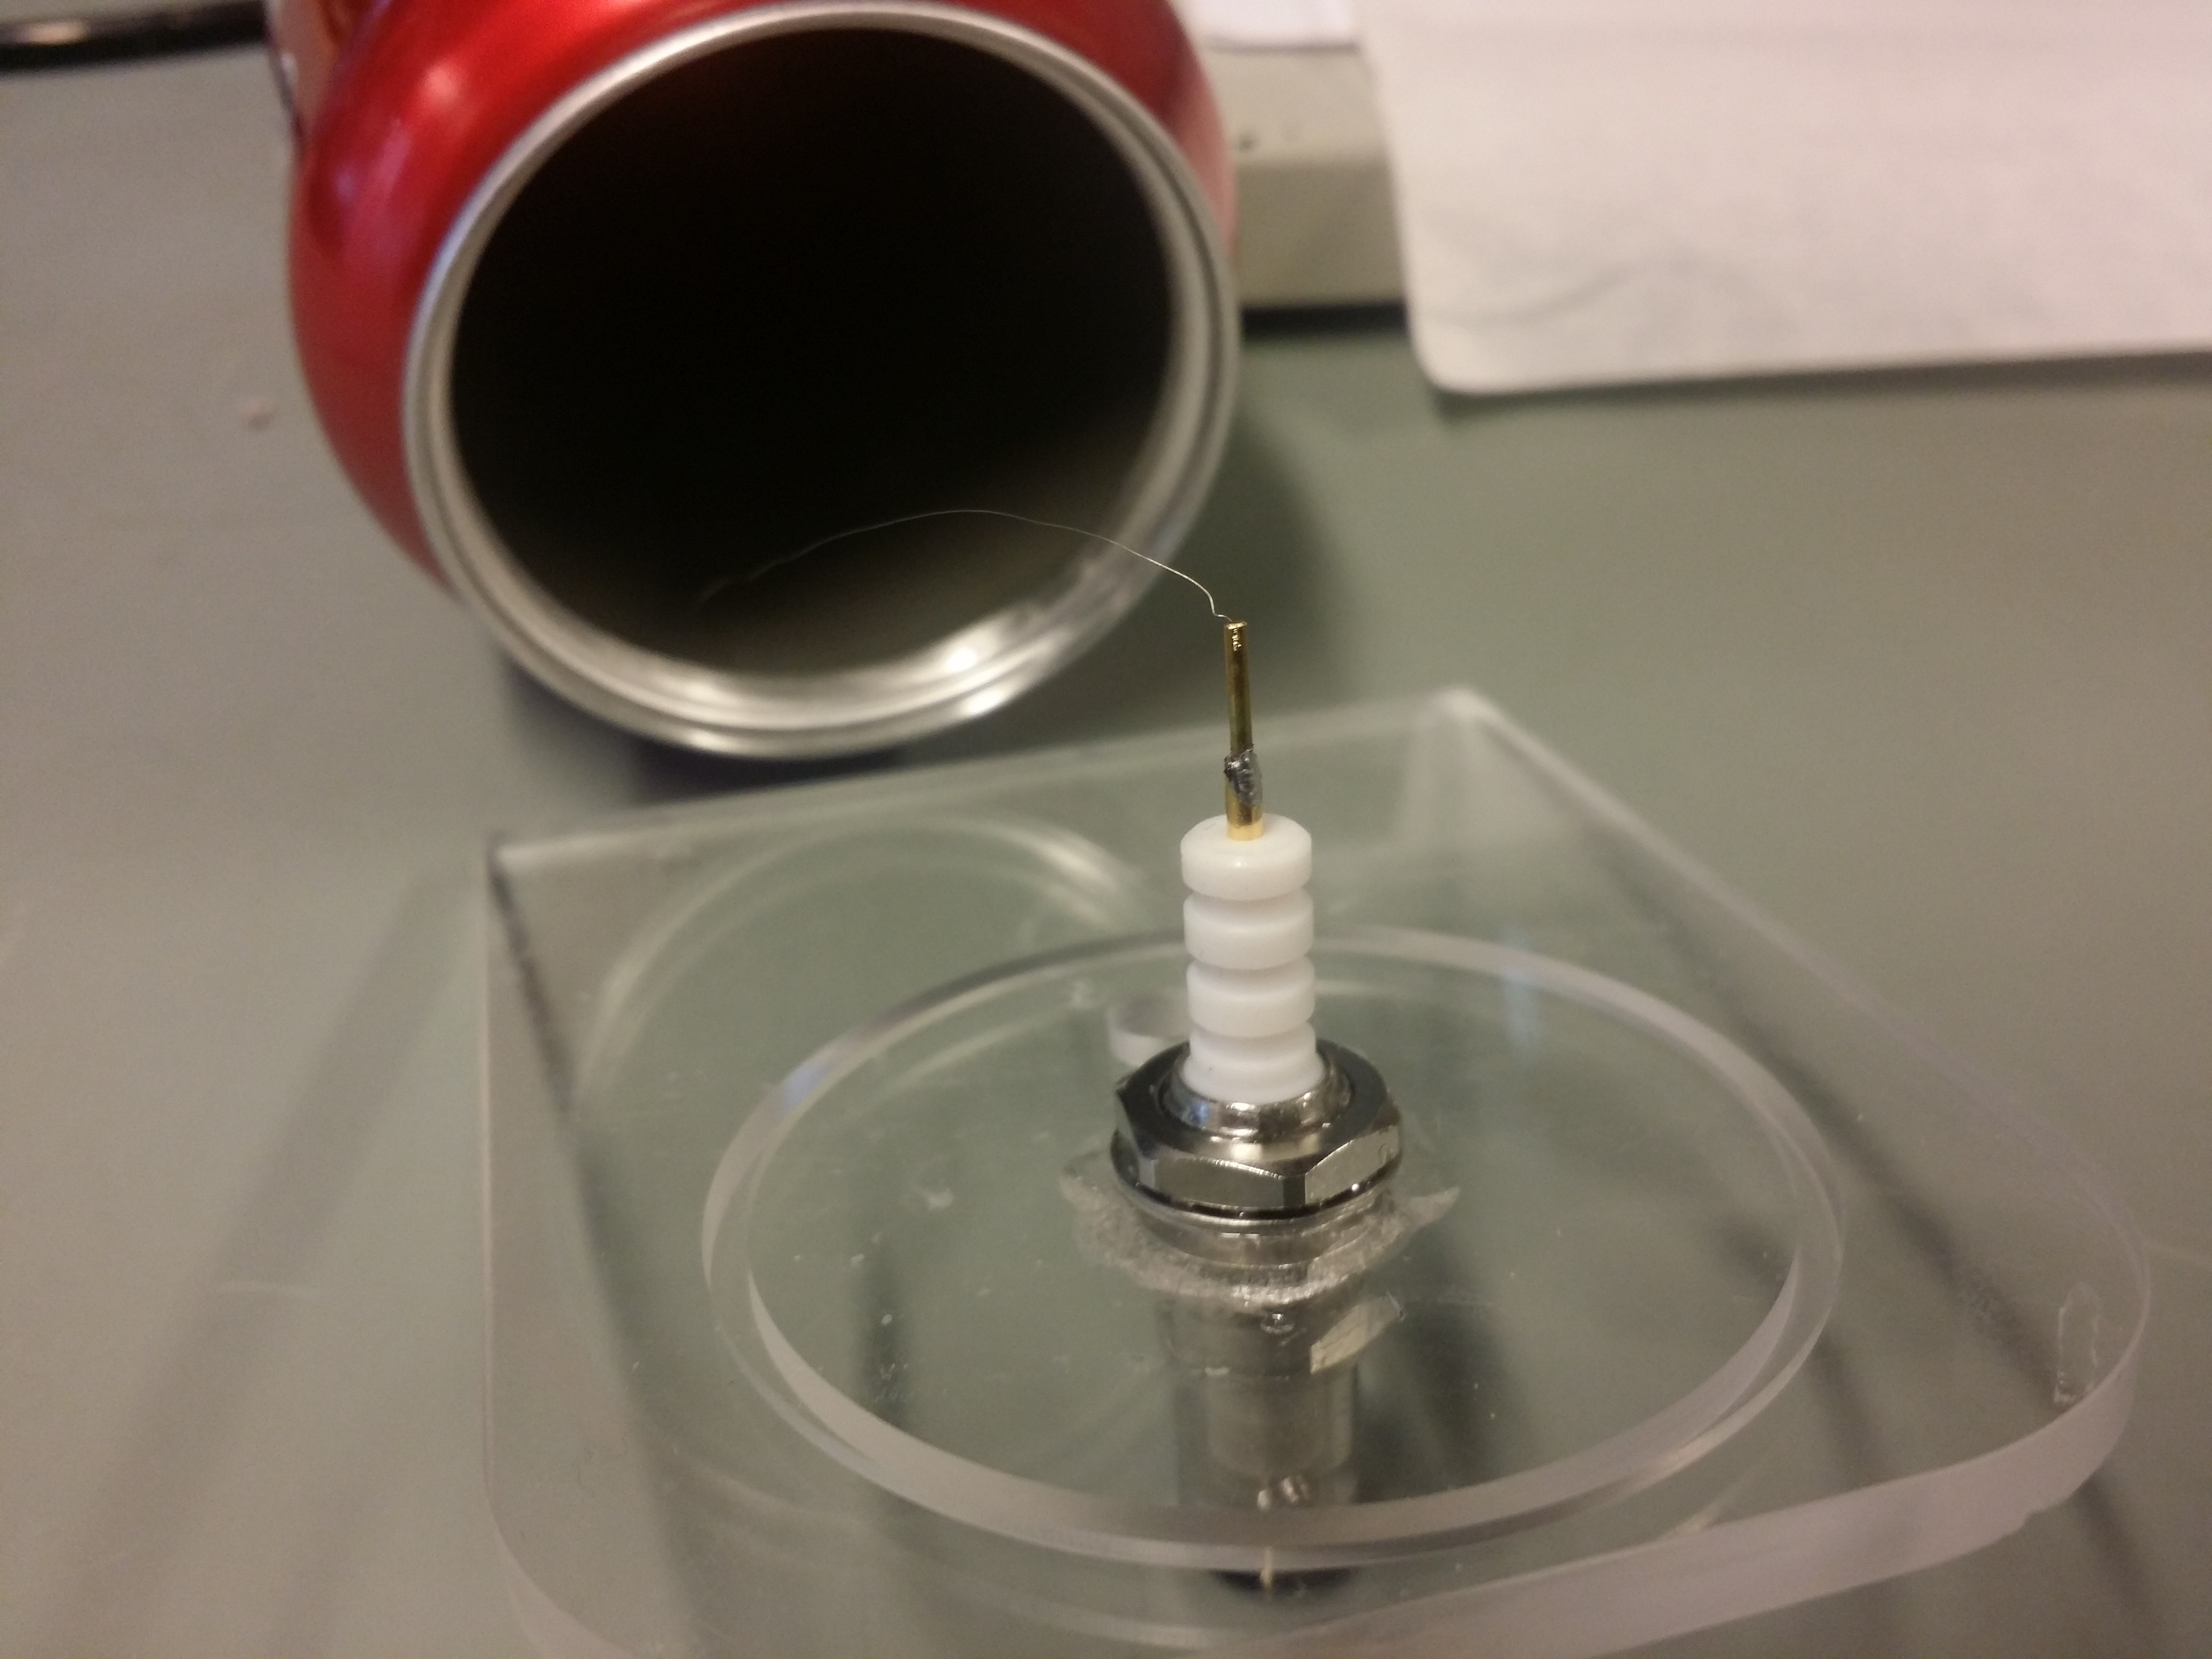
\includegraphics[width=\textwidth]{fig/IMG_20201117_121044.jpg}
\caption{The anode wire is soldered to the connector}
\label{fig:connector}
\end{subfigure}

\begin{subfigure}[t]{0.48\textwidth}
\centering
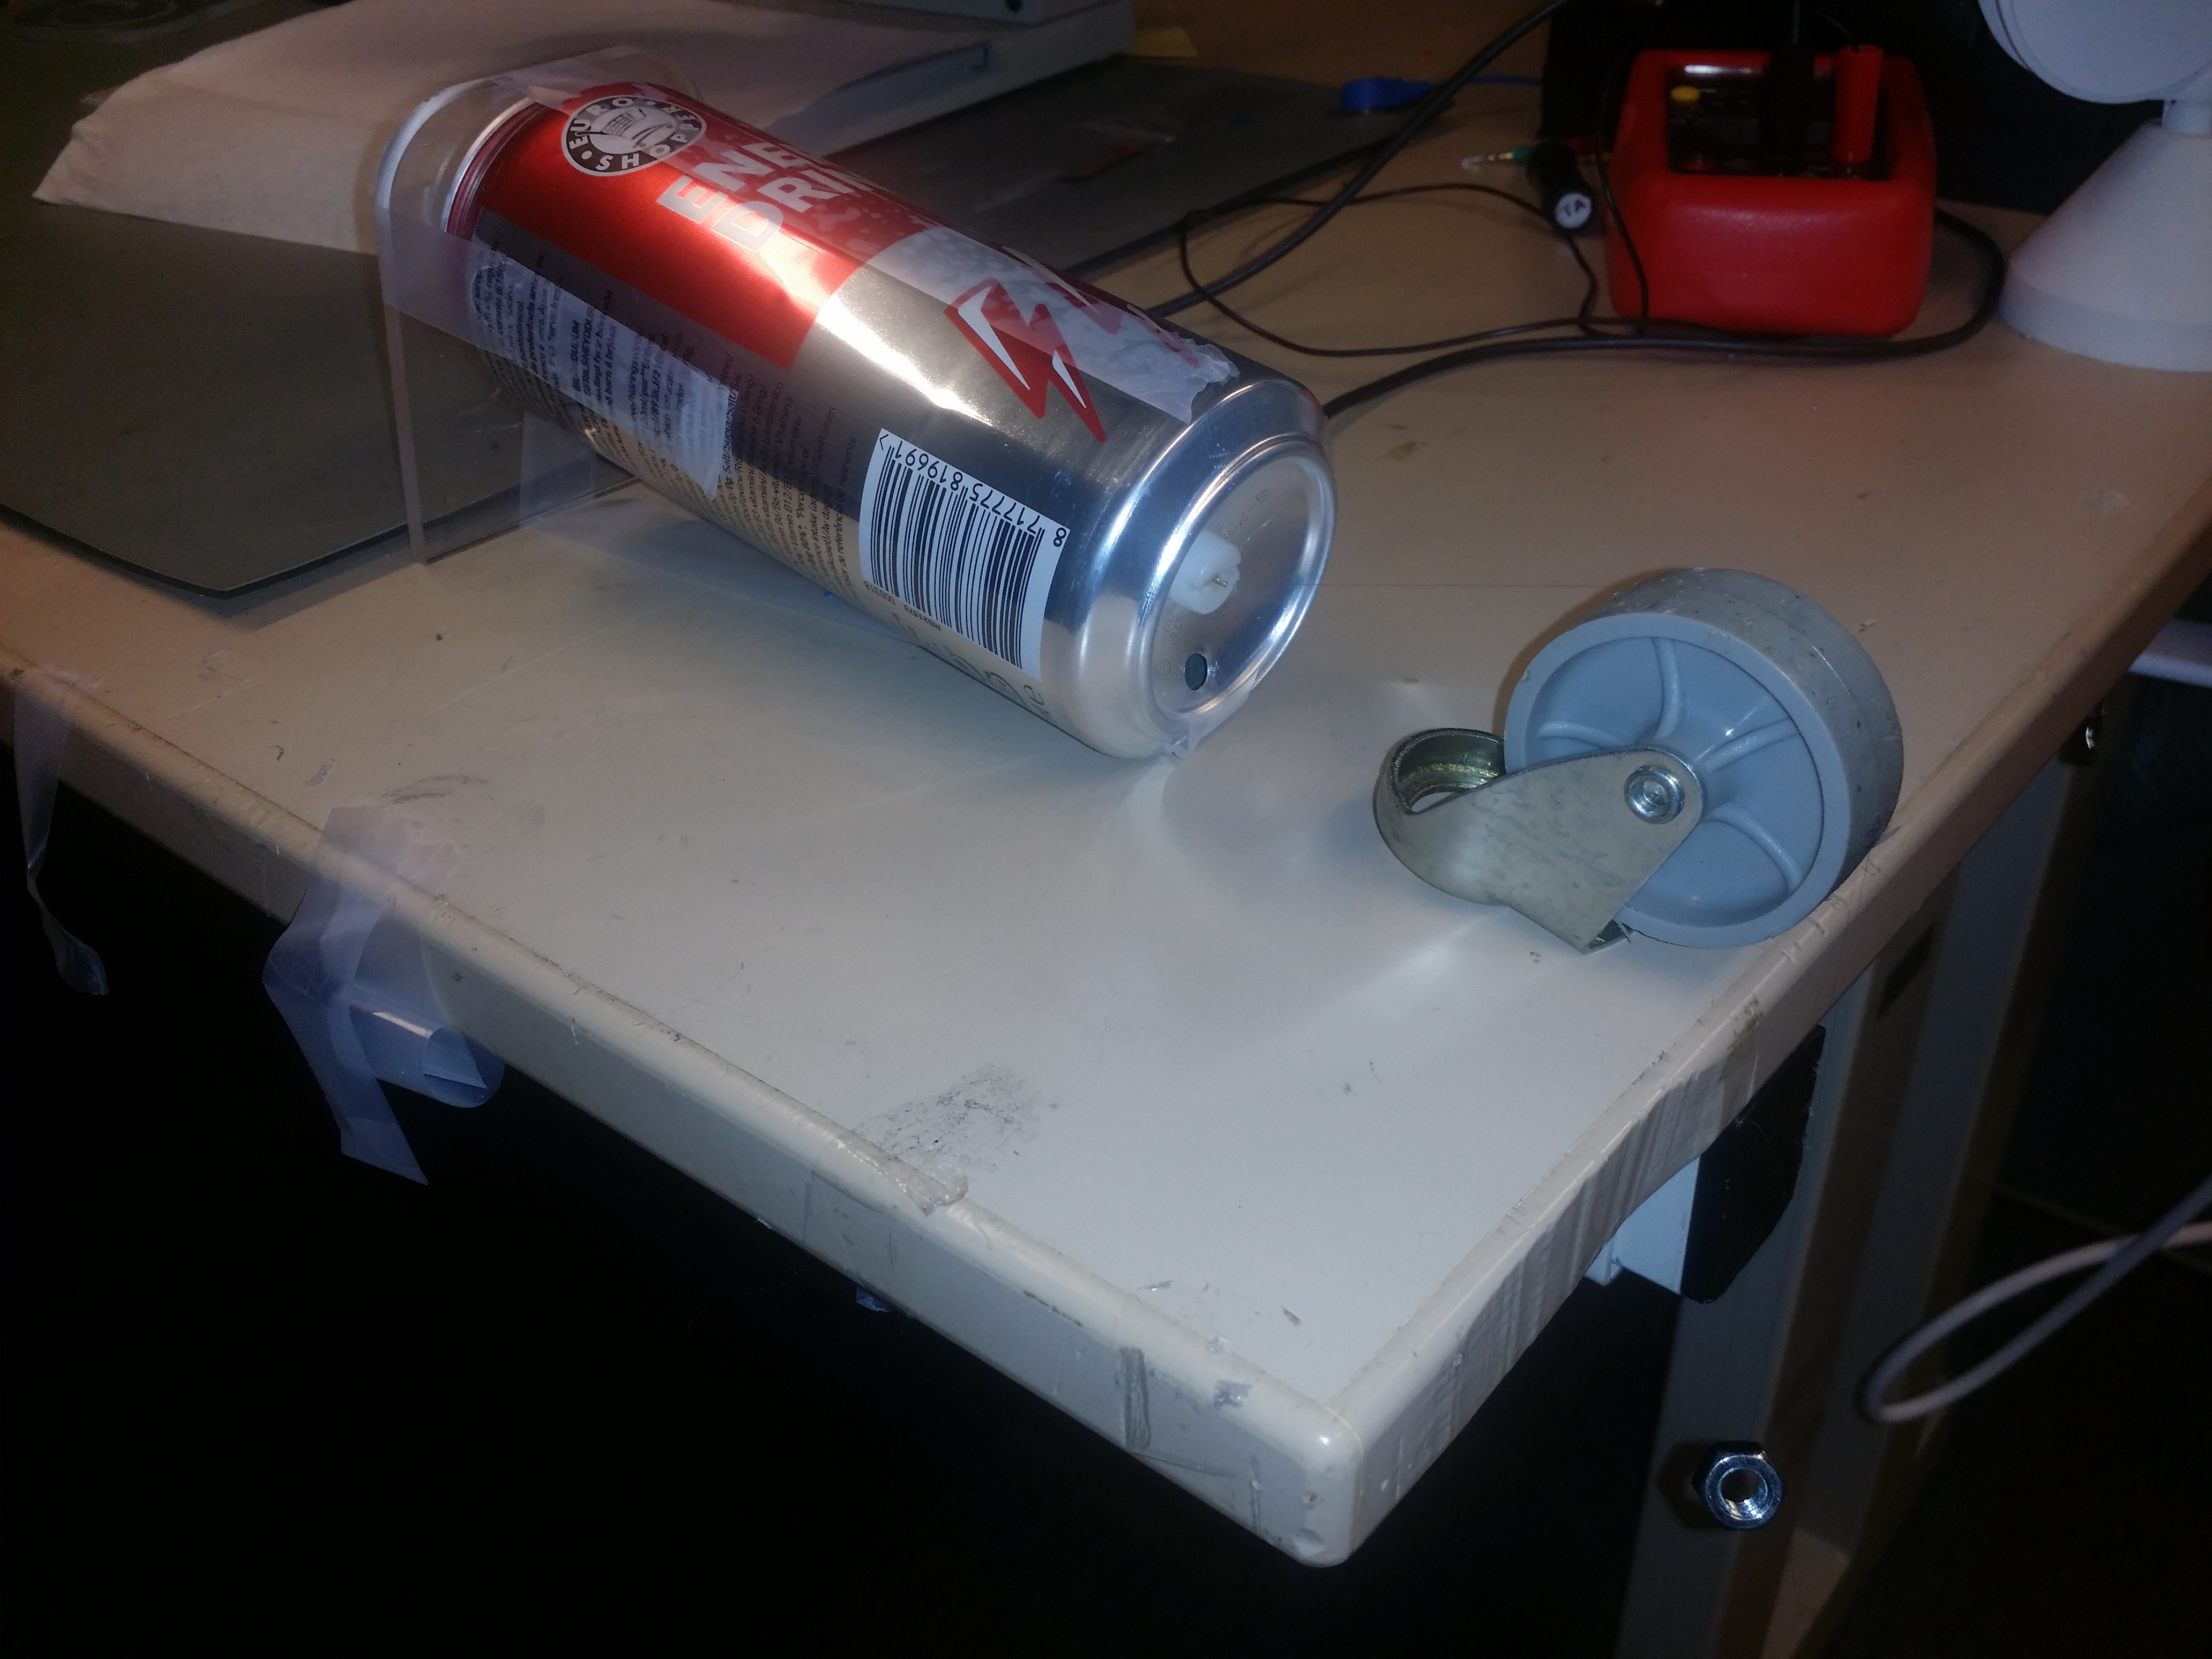
\includegraphics[width=\textwidth]{fig/IMG_20201123_104201.jpg}
\caption{Setup for tightening the anode wire}
\label{fig:tightening}
\end{subfigure}
%
\begin{subfigure}[t]{0.48\textwidth}
\centering
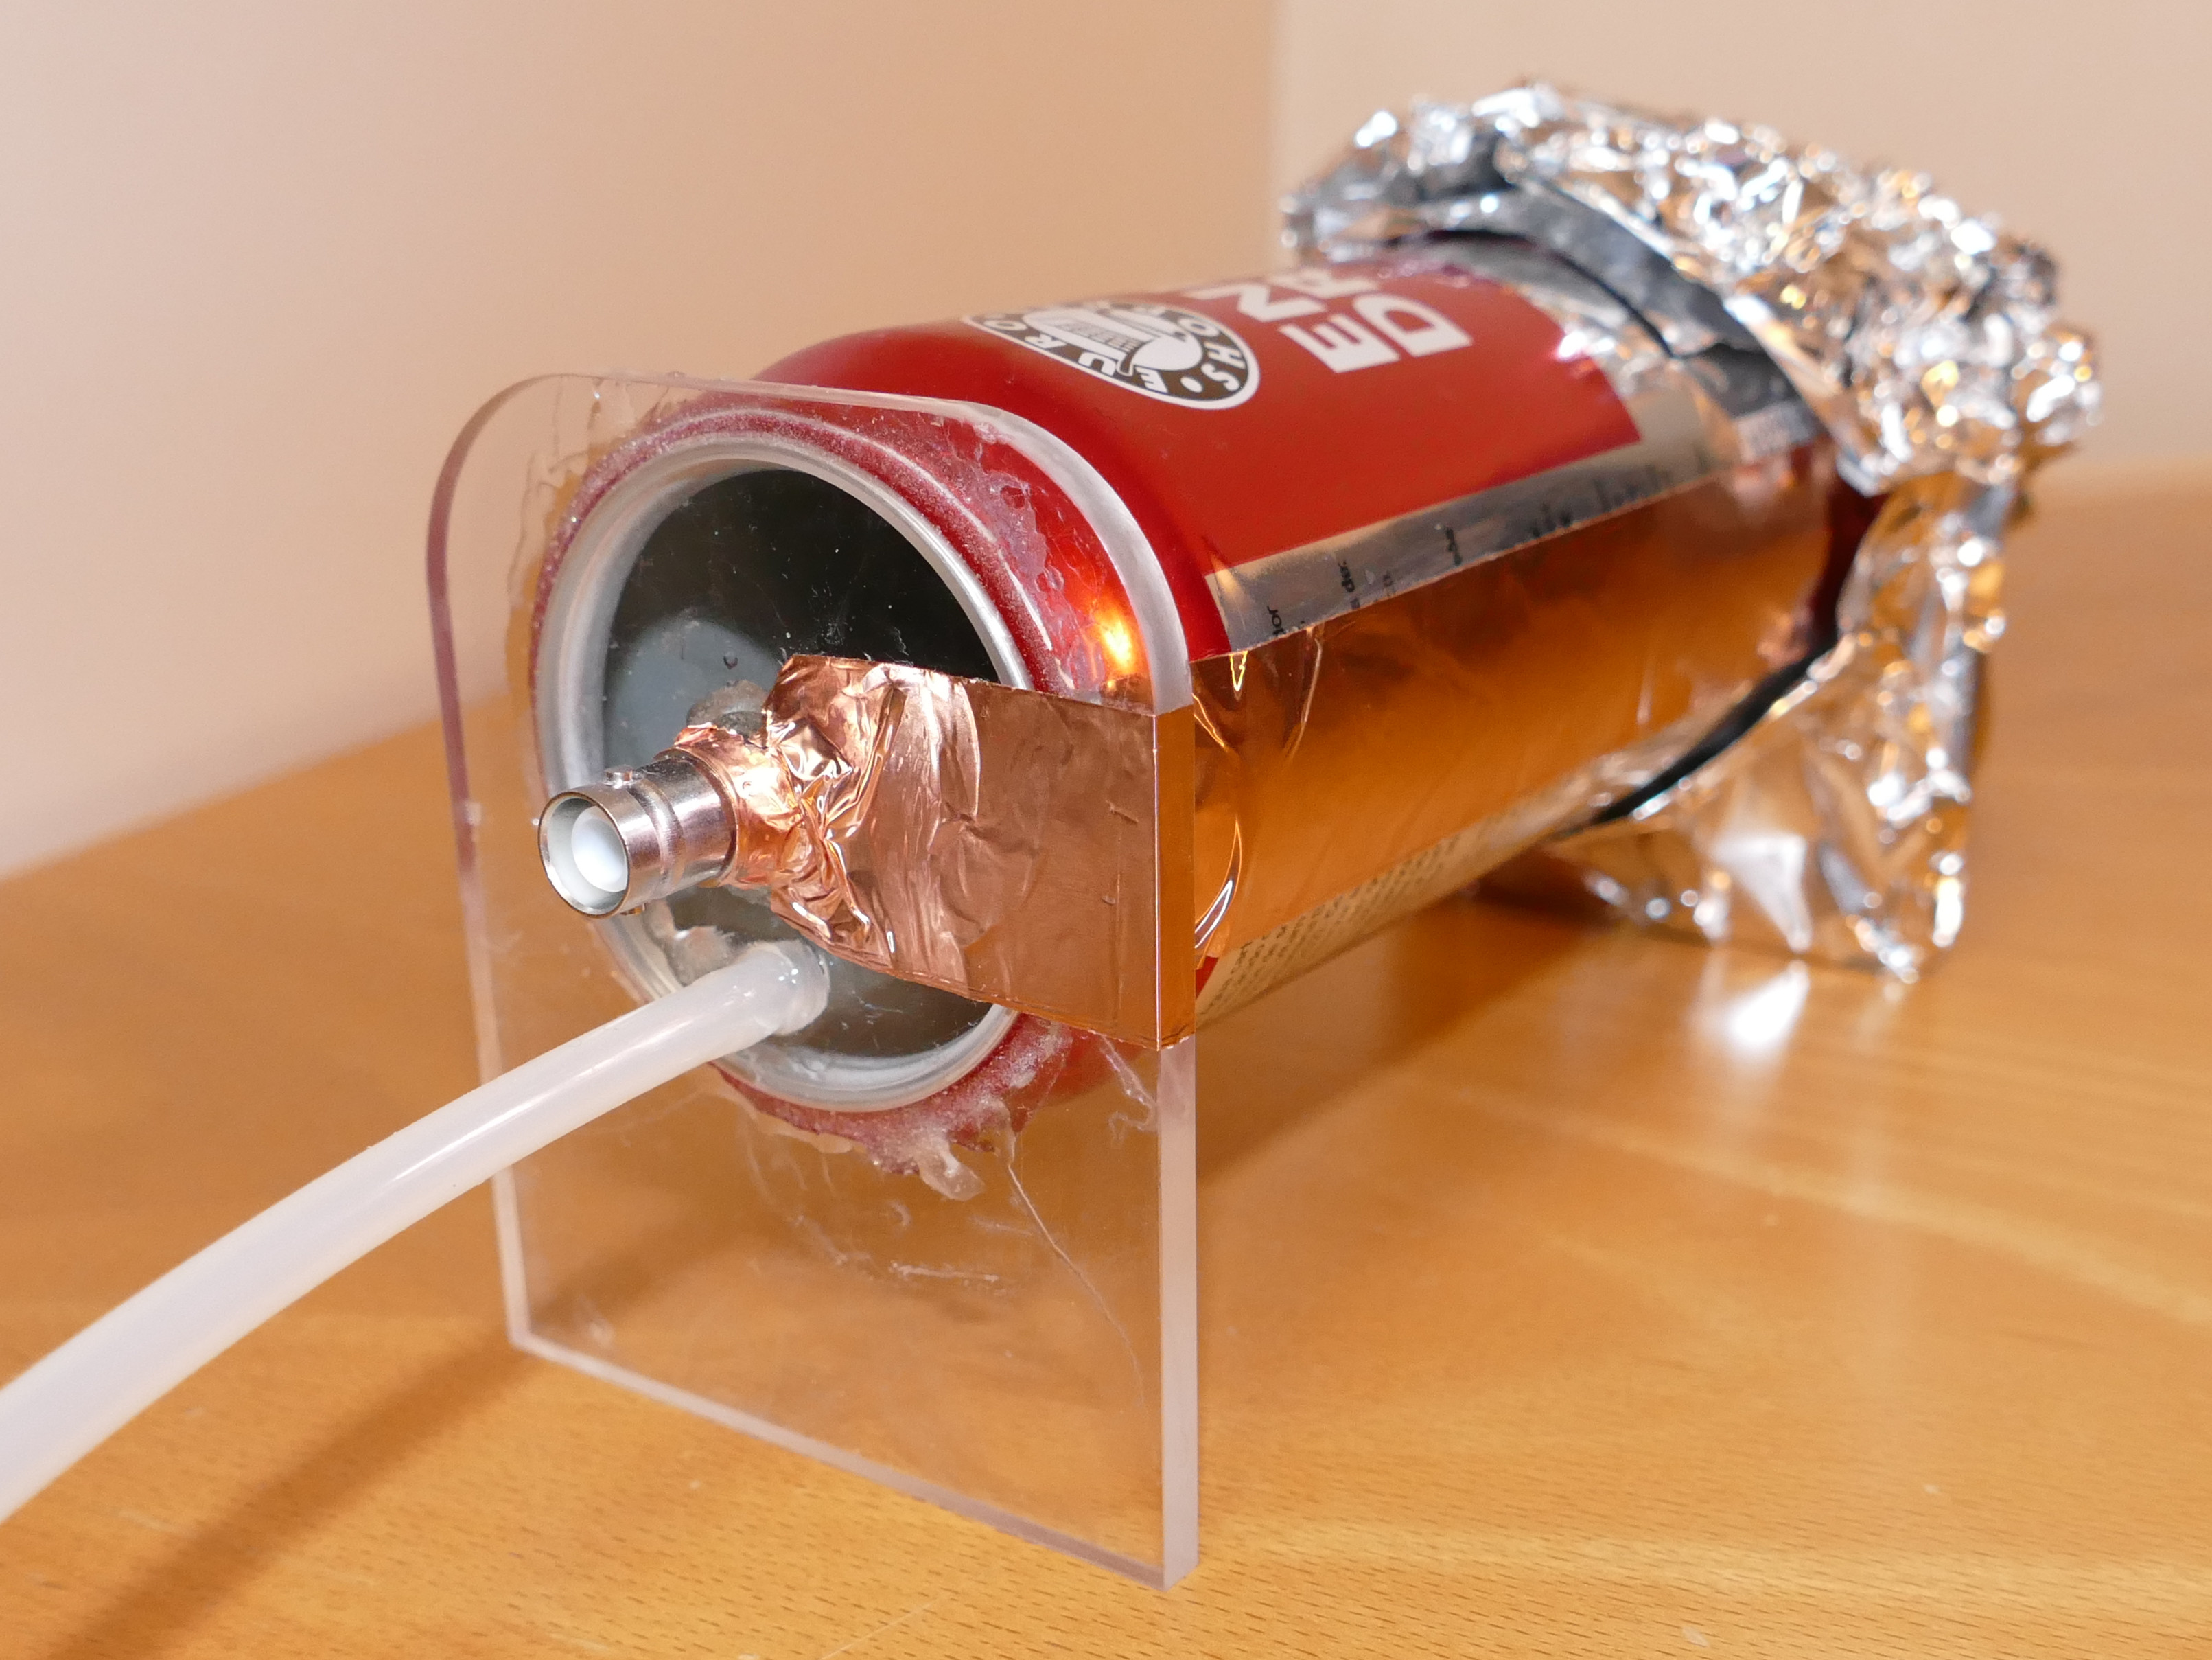
\includegraphics[width=\textwidth]{fig/P1170847-cropped.jpg}
\caption{Finished detector}
\label{fig:detector}
\end{subfigure}
%
\caption{Detector construction steps}
\end{figure}

The electric connection of the anode would be supplied by a high-voltage coaxial connector, which was attached to one of the
\href{https://en.wikipedia.org/wiki/Poly(methyl_methacrylate)}{plexiglass}
end caps with a nut and some epoxy glue.
The nut is sufficient to keep the connector in place, but the glue makes the connection airtight.
Once the connector was in place, the anode wire was pushed through the brass tube at the bottom of the can and pulled out of the top of the can.
The wire was then pushed through the shorter brass tube and twisted into a hook so that it stayed in place when the brass tube was pushed into the connector.
The electrical connection was then formed by soldering the brass tube and therefore also the wire to the connector as in figure \ref{fig:connector}
In this step one should be careful not to leave the end of the wire exposed from the solder, as such a sharp tip would cause high electric fields and therefore sparking.

Now the wire was in place, but it had to be tightened.
This was accomplished by taping the top cap to the can, knotting the wire around a nut and placing the wire over a wheel, as in figure \ref{fig:tightening}.
The tightening was then secured by soldering the wire to the brass tube, and then the remaining wire was cut.
In this step one should be careful to solder only as long as is needed for the solder to melt, as heating the wire for too long will cause it to break, as happened once during the manufacturing of this detector.
In the case of such an incident, a new wire has to be soldered to the high voltage connector.

Now the wire was in place, and the detector had to be sealed.
Large amounts of epoxy were used to attach the end caps, and office tape to hold the caps in place.
In this step one should wait for the epoxy to dry properly before removing the top cap, as otherwise the cap may move and break the strained anode wire.
Once the epoxy of the caps was dry, some more was added to ensure airtightness.
Then a pipe was attached to the hole on each of the end caps.

Finally one side of the can was brushed with sandpaper and attached a piece of copper tape so that it went all the way to the shielding of the high voltage connector.
This established an electrical connection between the ground and the can.
It should be noted that the copper tape should be put on a different side than on which the radiation source is placed, as the copper tape would otherwise absorb some of the radiation.
A piece of aluminum foil was put over the bottom of the can to provide additional shielding from electromagnetic interference, as the end of the anode wire slightly extrudes from within the can.



\clearpage
\subsection{Calibration}
\label{setup_calibration}
The detector and readout electronics had to be calibrated to establish a relationship between the channels of the multichannel analyzer and the energies of the incoming radiation.
The setup consisted of an
\href{https://iseg-hv.com/en/products/detail/NHR}{Iseg NHR 42 60r}
high voltage power supply,
\href{https://www.ortec-online.com/products/electronics/preamplifiers/142a-b-c}{Ortec 142}
pre-amplifier,
\href{https://www.ortec-online.com/products/electronics/amplifiers/855}{Ortec 855}
dual spectral amplifier,
\href{https://www.amptek.com/products/multichannel-analyzers/mca-8000d-digital-multichannel-analyzer}{Amptek MCA-8000D}
digital multichannel analyzer and
\href{https://teledynelecroy.com/oscilloscope/wavesurfer-3000z-oscilloscopes/wavesurfer-3024z}{Lecroy WaveSurfer 3024z} oscilloscope (200 MHz).
The electrical connections of the setup used for both calibration and the measurements are illustrated in figure \ref{fig:connections}, except that for the electronics calibration the oscilloscope was connected directly to the output of the pulser.

\begin{figure}[ht!]
\centering
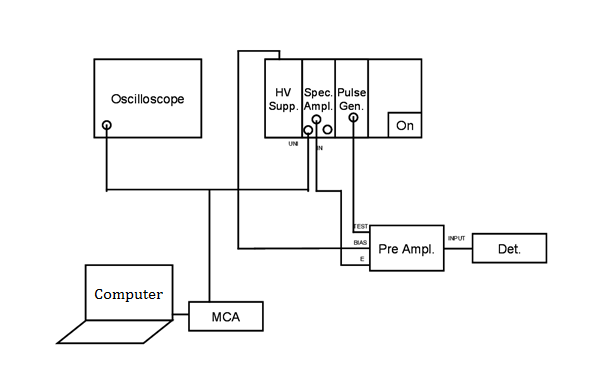
\includegraphics[width=\textwidth]{fig/instructions/connections.png}
\caption{Electrical connections of the setup \cite{instructions}}
% TODO draw own one with vector graphics}
\label{fig:connections}
\end{figure}

\FloatBarrier
The first step was the calibration of the multichannel analyzer to the collected charge.
This was done by setting the bias voltage to zero and attaching a pulse generator to the amplifier input, and an oscilloscope and the multichannel analyzer to its output, as in figure \ref{fig:pulser_setup}.
The voltage over a capacitor is defined by the equation $V = \frac{Q}{C}$, where $Q$ is the collected charge, $C$ is the 1 pF test input capacitance of the pre-amplifier.
Therefore the collected charge is defined by $Q = CV$, where $V$ is the output pulse height measured with the oscilloscope.
The pulse height was determined by comparing the value of an exponential fit at the peak time to the average voltage before the pulse.
These are illustrated in figure \ref{fig:cal_trace}.

\begin{figure}[ht!]
\centering
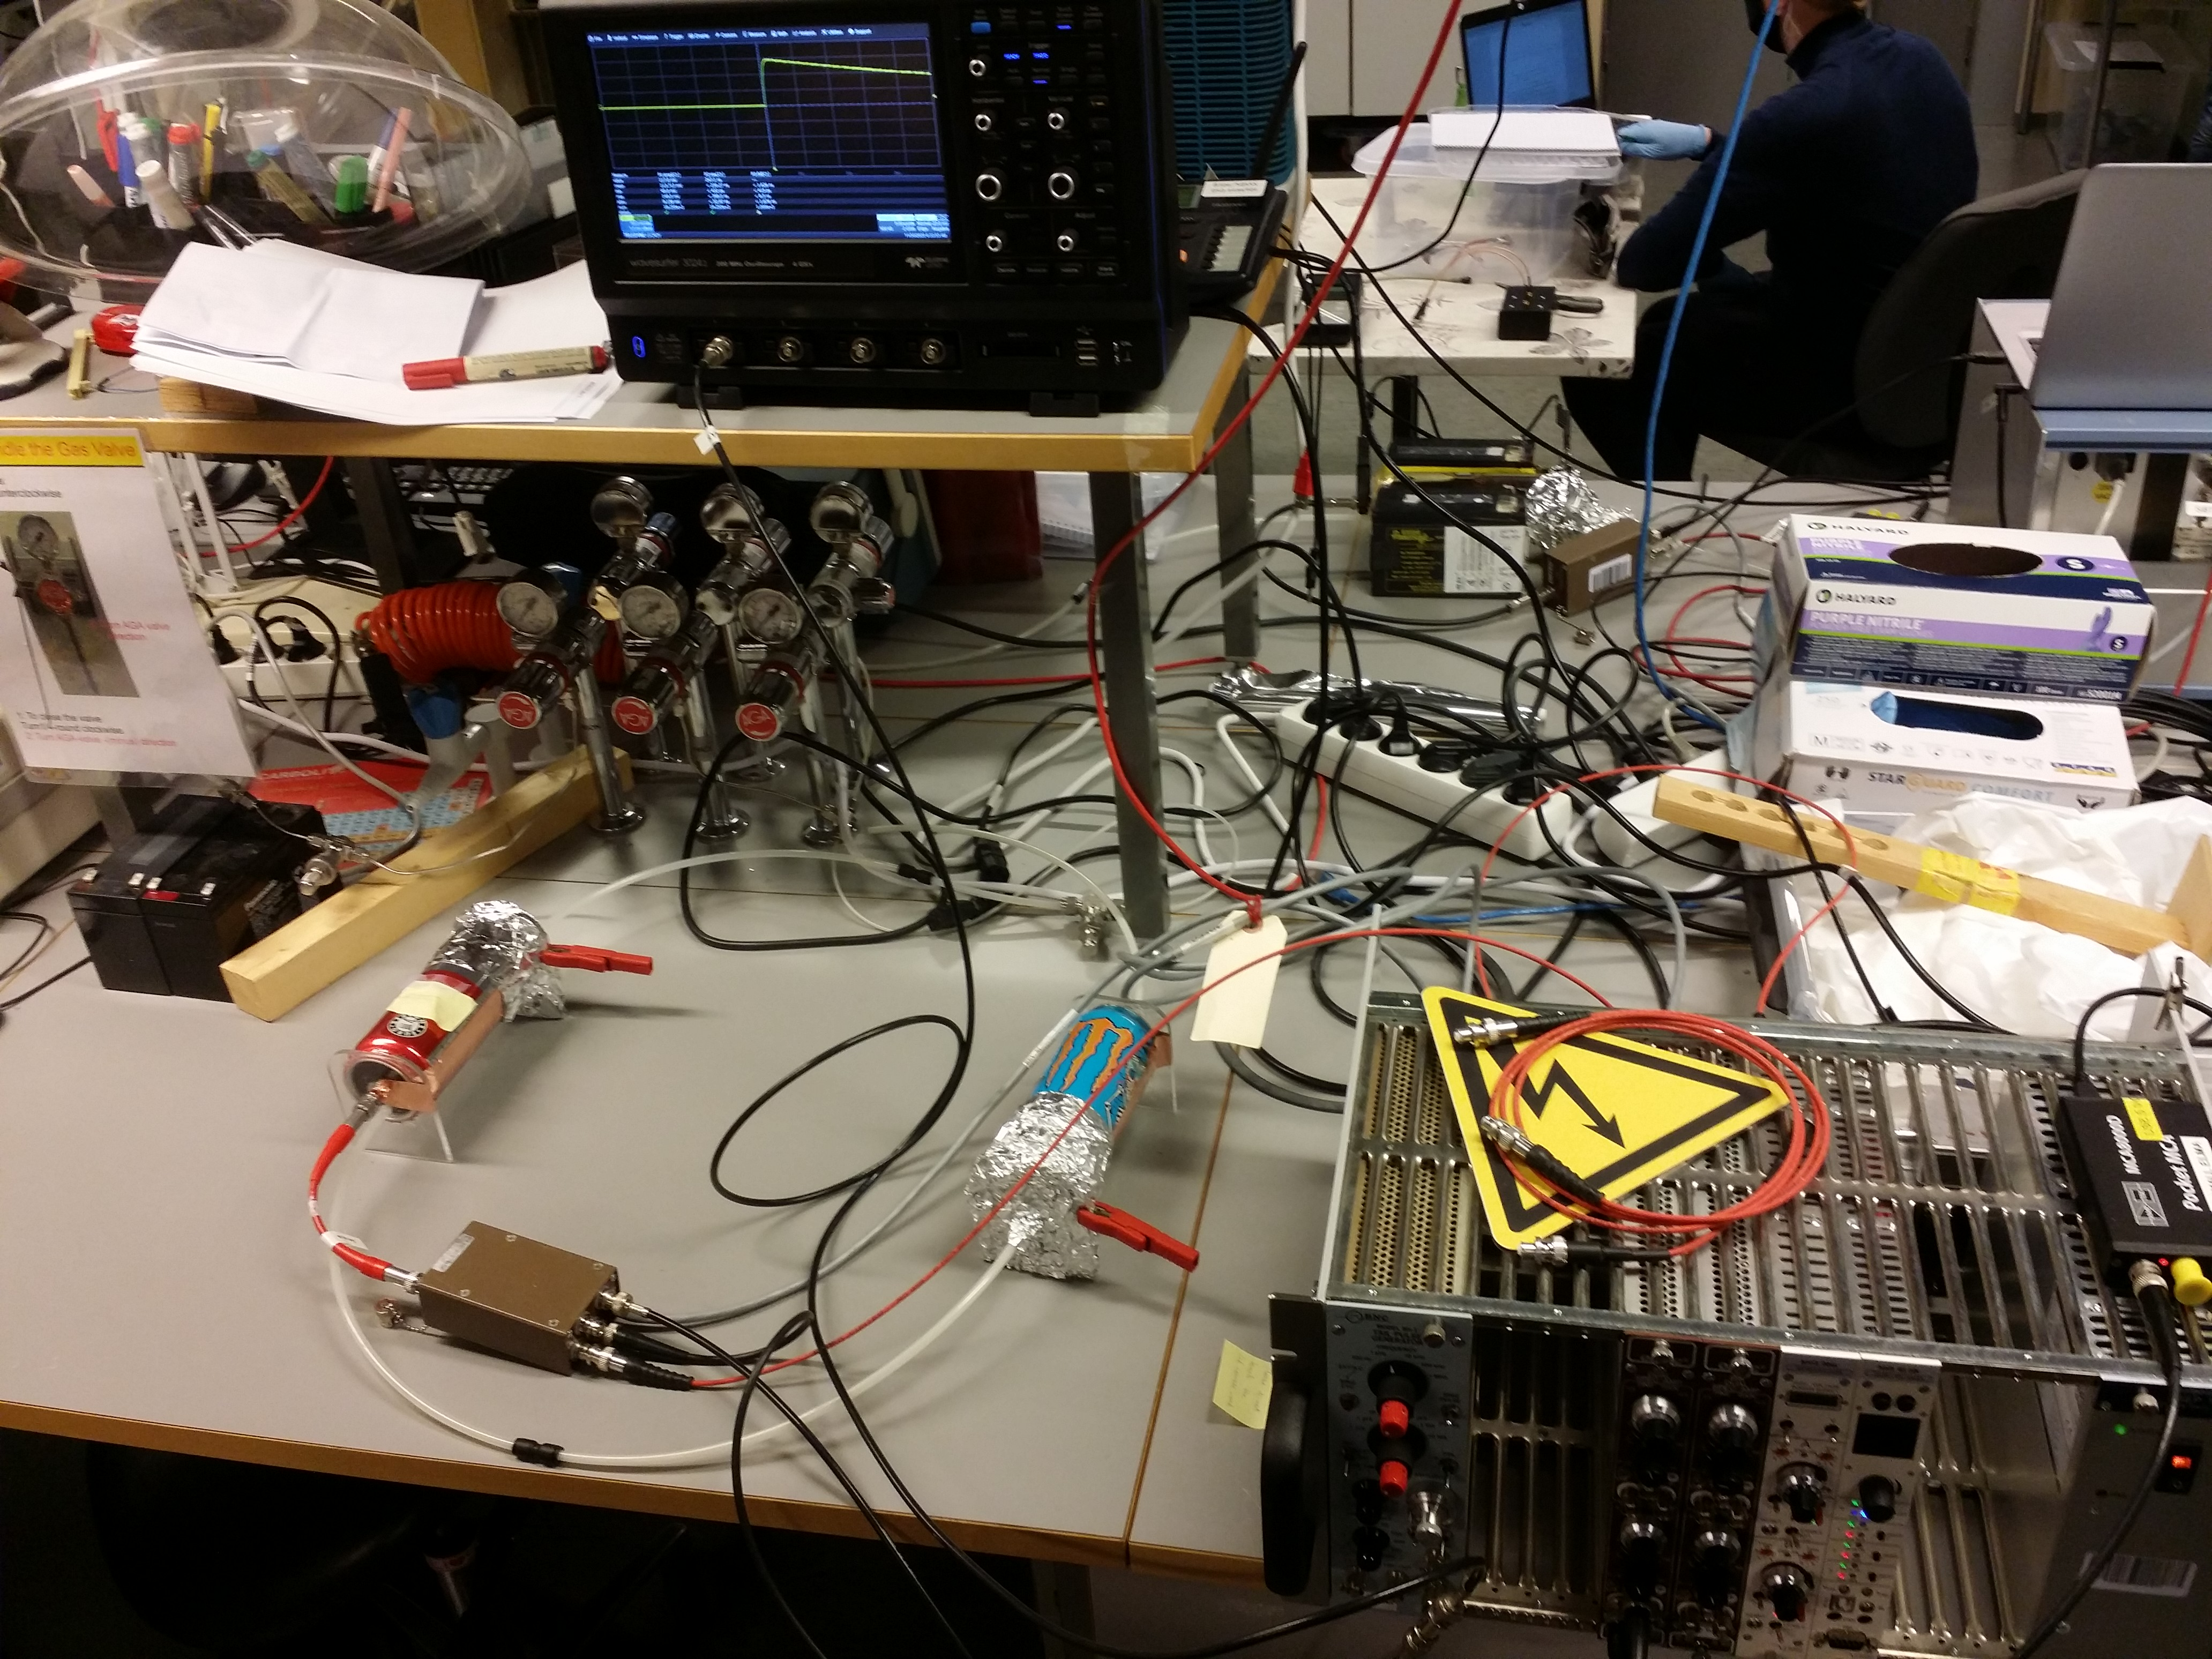
\includegraphics[width=0.8\textwidth]{fig/IMG_20201130_135000.jpg}
\caption{Setup for testing with an external pulser}
\label{fig:pulser_setup}
\end{figure}

\begin{figure}[ht!]
\centering
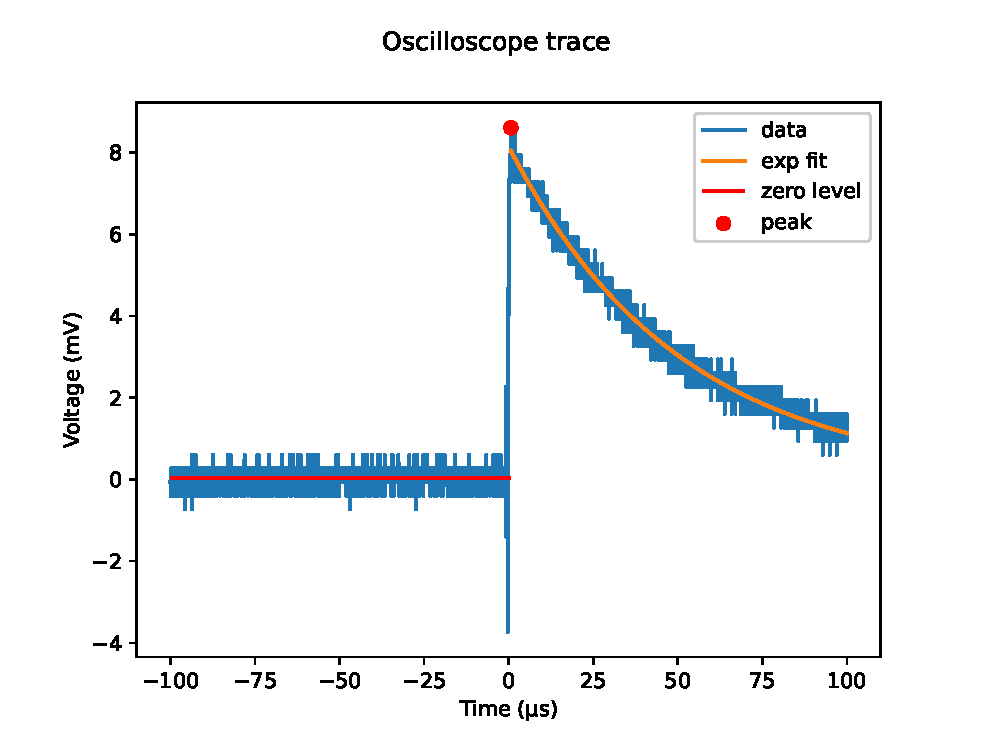
\includegraphics[width=\textwidth]{fig/python/calibration_trace.eps}
\caption{An oscilloscope trace for the calibration}
\label{fig:cal_trace}
\end{figure}



\FloatBarrier
\subsection{Measurements with radiation sources}
\label{setup_testing}
For the testing with radiation sources the electrical connections were the same as for the calibration, except that the pulse generator was removed and that the oscilloscope was attached to the output of the spectral amplifier.
The detector was placed within a lead shielding that consisted of two lead-acid batteries, and the radioactive source was placed on top, as in figure \ref{fig:setup_testing}.
For the $^{241}$Am source a thick metal sheet with a thin slit had to be used as a collimator to reduce the intensity of the radiation.
Without the attenuator the pulses would pile up so that individual pulses would no longer be detectable separately for energy measurement.
Due to its different enclosure and higher activity, the $^{241}$Am source also required the use of additional lead shielding around the setup to prevent unnecessary user exposure to the radiation.

\begin{figure}[ht!]
\centering
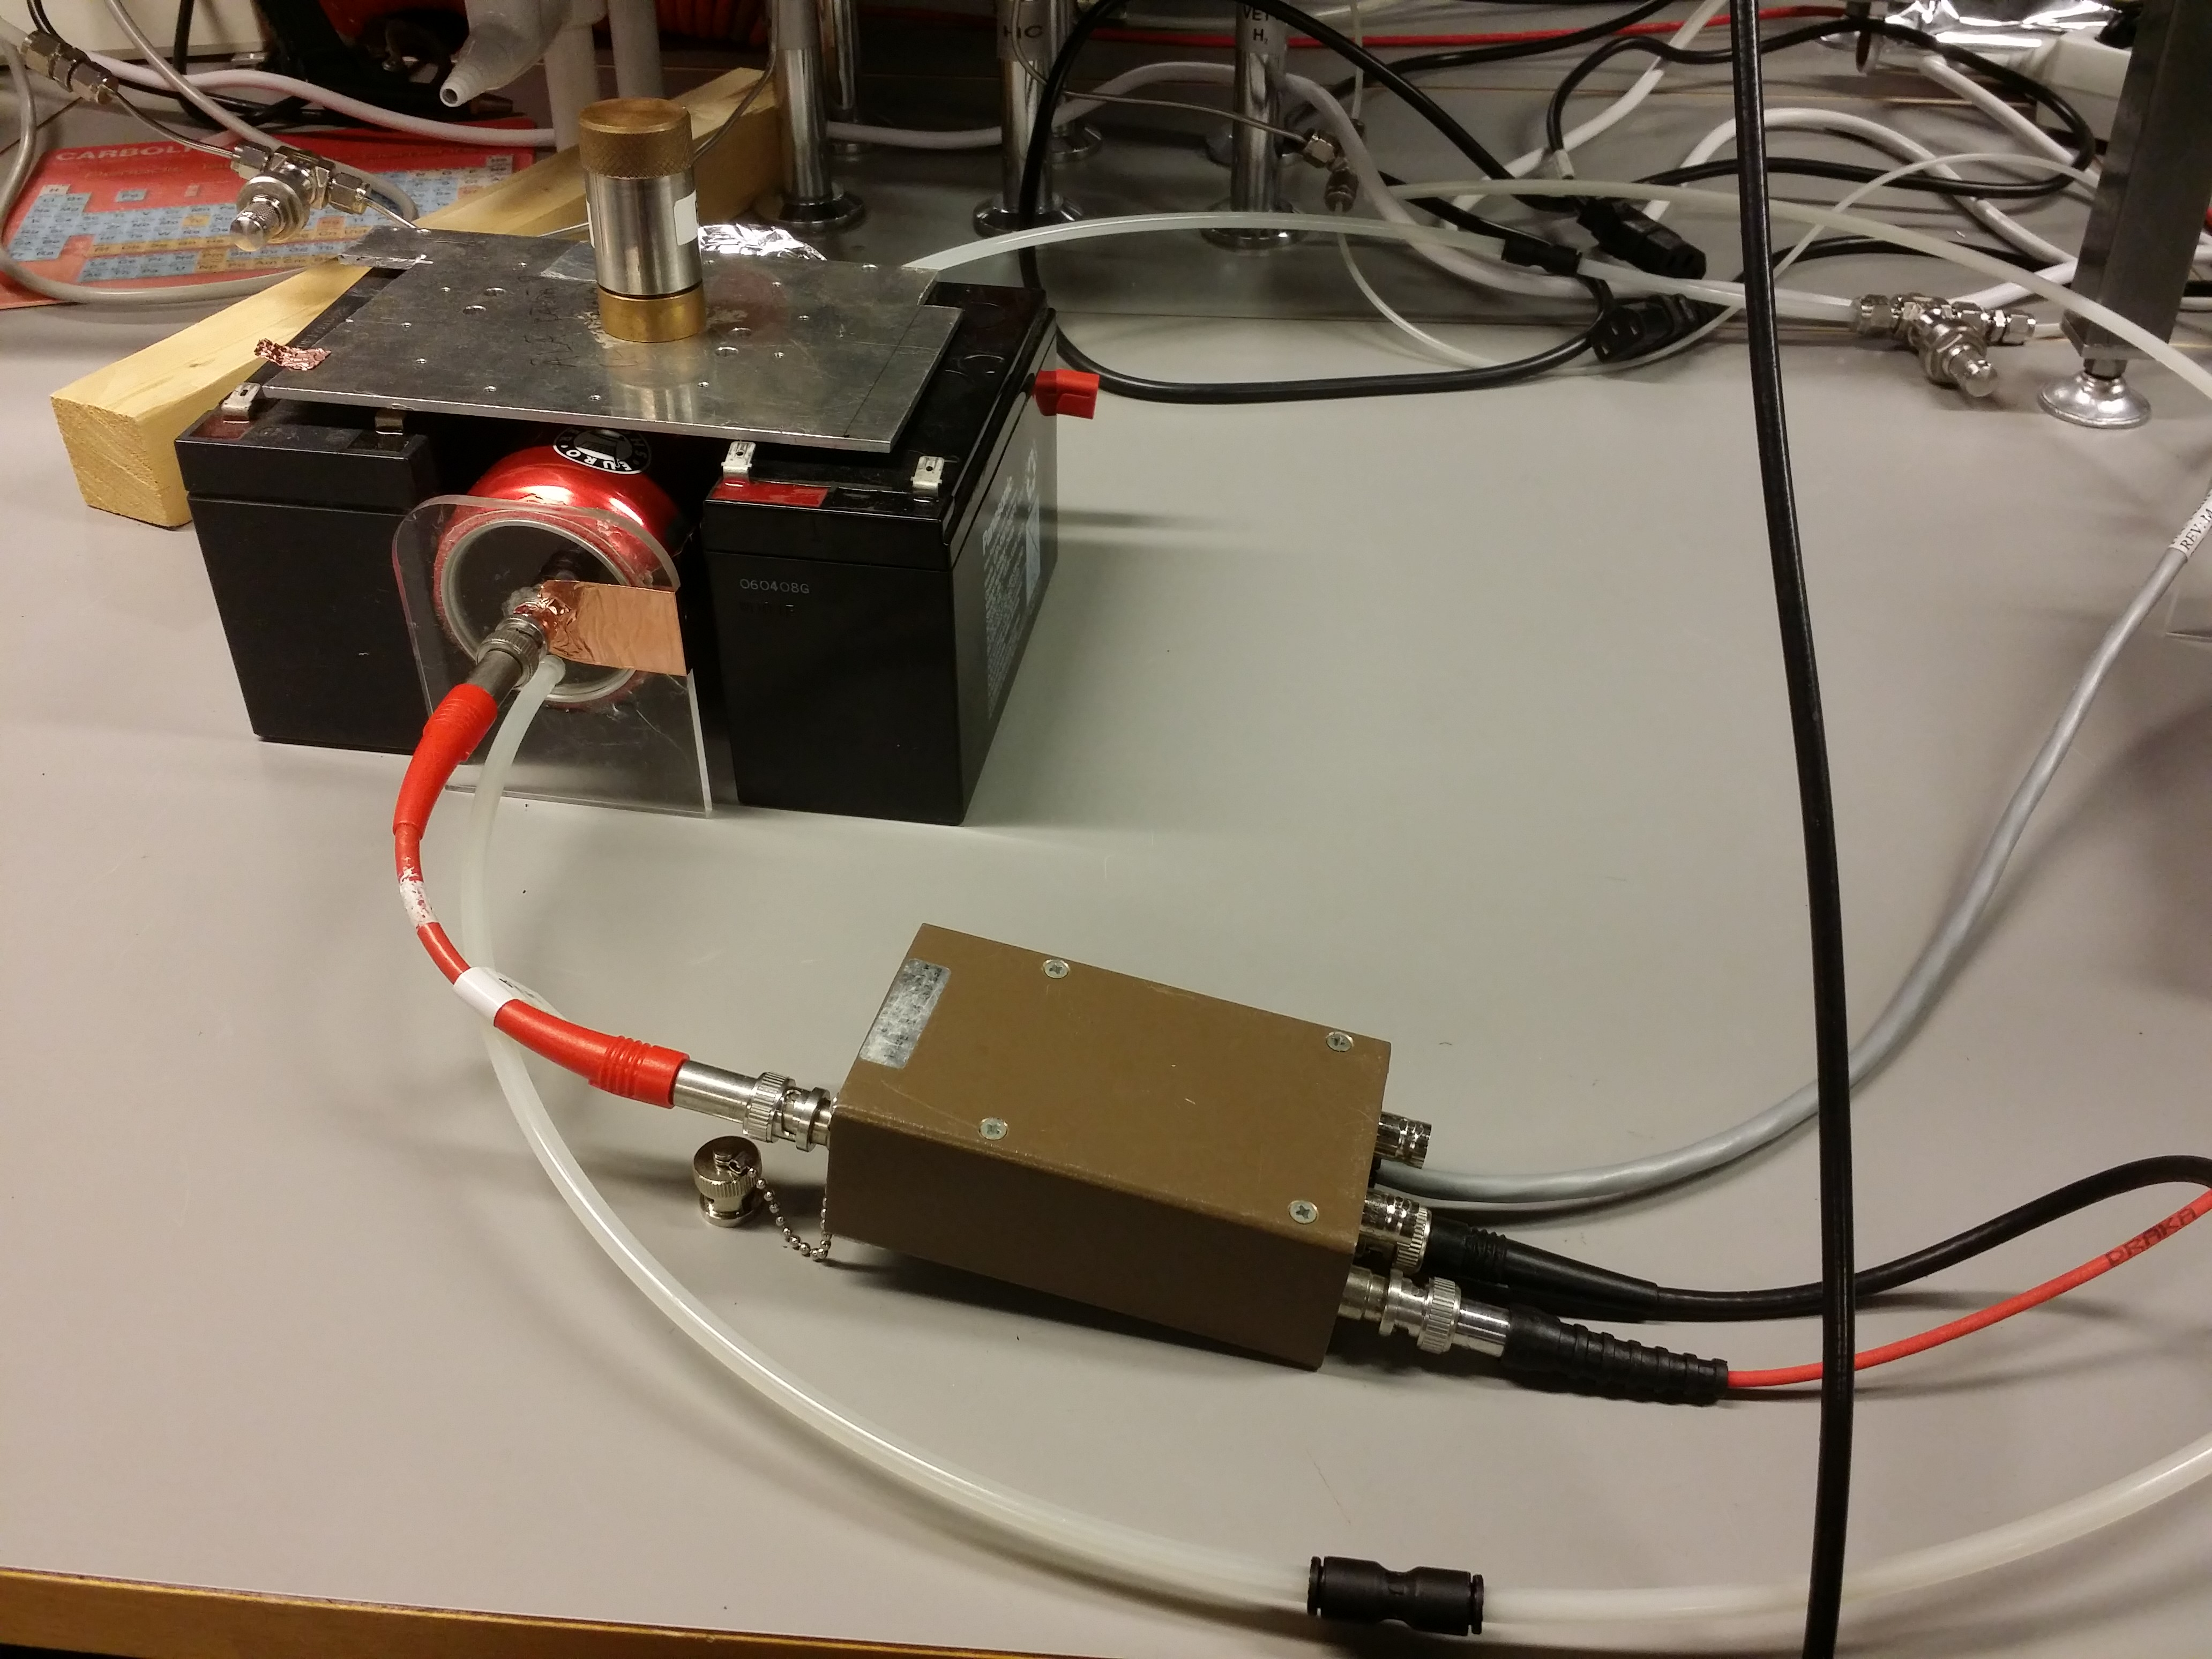
\includegraphics[width=0.8\textwidth]{fig/IMG_20201130_144418.jpg}
\caption{Setup for testing with an $^{55}$Fe source and the rack-mounted amplifier}
\label{fig:setup_testing}
\end{figure}



\clearpage
\section{Results and discussion}
\label{results}
This chapter discusses the measurement results of the setups described in chapter \ref{assembly}.
The code used for the data analysis is available in the GitHub repository. \cite{repo}


\subsection{Calibration}
\label{results_calibration}
By varying the voltage of the test pulse we get the relationship between the peak MCA channel and the collected charge as in figure \ref{fig:mca_calibration}.
The error bars represent the standard deviation of five measurements except for one data point which had four successful measurement and one data point which had only two due failed data captures that were not noticed until analyzing the data.
To this data we can make the linear fit
\begin{equation}
Q = g \cdot \text{Channel}_\text{MCA} + h.
\label{eq:calibration}
\end{equation}
We used orthogonal distance regression to account for both the differential nonlinearity of the MCA and the standard deviation of the measured voltages for each pulser setting.
The
\href{https://en.wikipedia.org/wiki/Differential_nonlinearity}{differential nonlinearity}
of the MCA is 0.6 \%, and the
\href{https://en.wikipedia.org/wiki/Integral_nonlinearity}{integral nonlinearity}
is 0.02 \%.
The resulting error bars for the collected charge are significantly tighter than for Winkler et al., as we extracted the pulse heights and their standard deviations with software instead of measuring and estimating the error by eye.
For the fit parameters we get the values $g = 1.46 \cdot 10^{-4} \pm 4.81 \cdot 10^{-7}$ pC/channel and $h = -1.04 \cdot 10^{-4} \pm 6.99 \cdot 10^{-5}$ pC.
The calibration of the pulser was also investigated, and the results are discussed in appendix \ref{pulser_calibration}.


\begin{figure}[ht!]
\centering
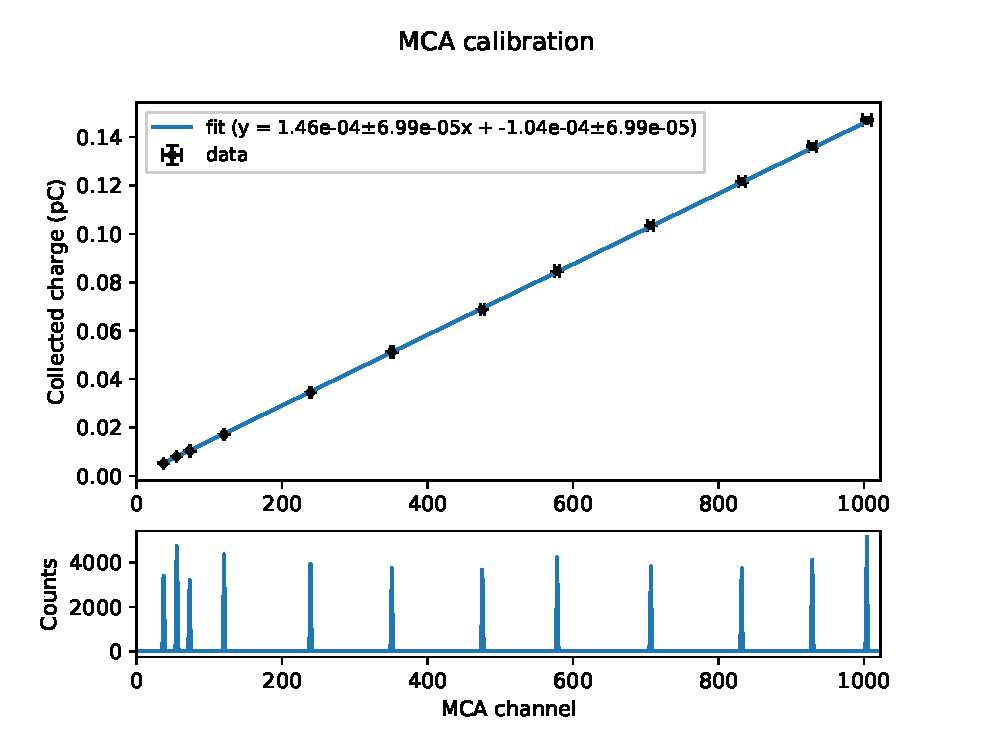
\includegraphics[width=\textwidth]{fig/python/mca_calibration.eps}
\caption{MCA calibration: collected charge as a function of the MCA channel with a linear fit, and a histogram of the measured detection counts}
\label{fig:mca_calibration}
\end{figure}


\clearpage
\subsection{High voltage sweep}
\label{results_hv}
To find the optimal settings for the detector we tested it with several voltages and gain values.
With the $^{241}$Am source we obtained the spectra in figure \ref{fig:am_scan_fits} and for the $^{55}$Fe source the data in figure \ref{fig:fe_scan_fits}.
For $^{55}$Fe the tested voltage range was 1603--2301 V, and for $^{241}$Am 1152--2301 V, as within this range suitable gain values were available to fit the signal within the range of the multichannel analyzer.
The voltage and coarse gain values for each measurement are provided in the figures.
The fine gain of the amplifier was held constant.

\begin{figure}[ht!]
\centering
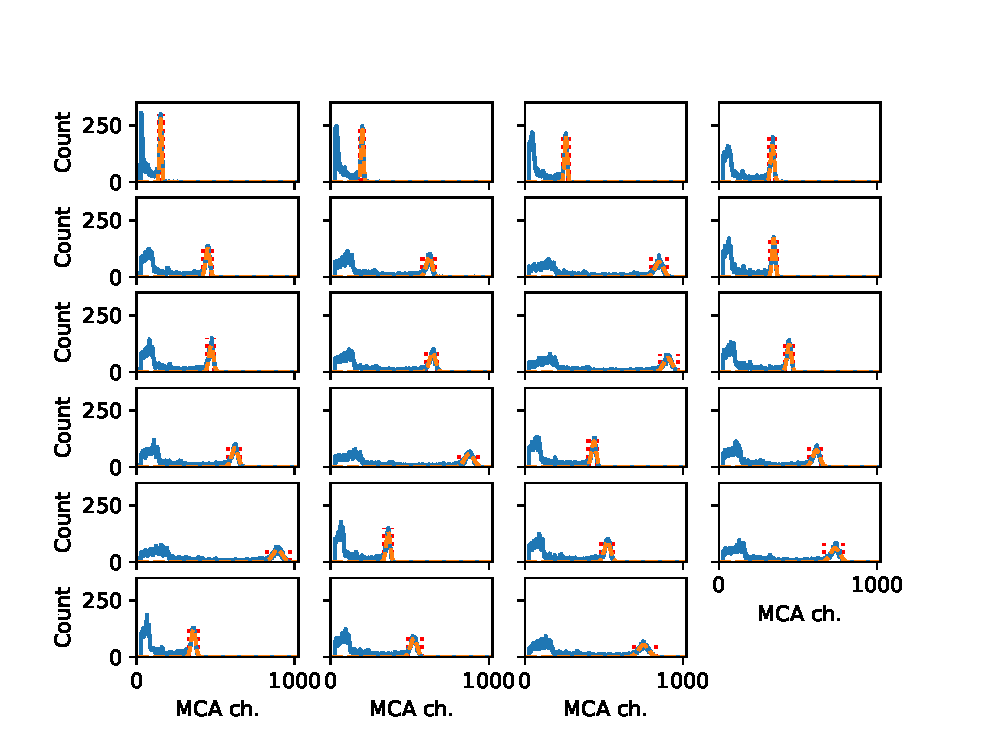
\includegraphics[width=\textwidth]{fig/python/am_scan_fits.eps}
\caption{$^{241}$Am voltage scan data}
\label{fig:am_scan_fits}
\end{figure}

\begin{figure}[ht!]
\centering
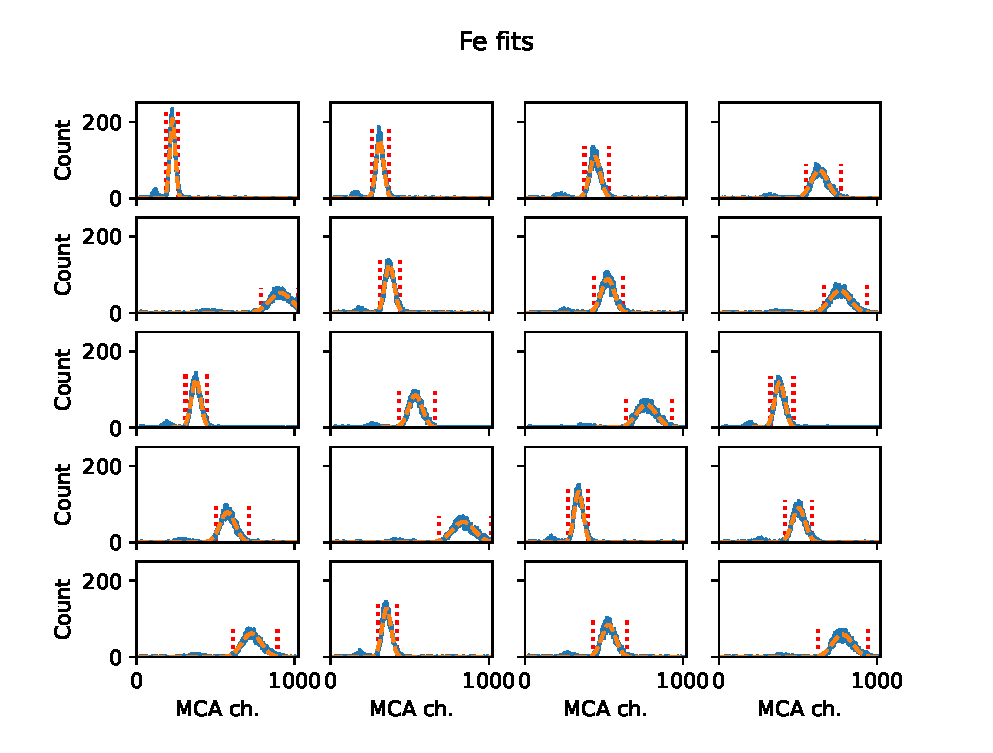
\includegraphics[width=\textwidth]{fig/python/fe_scan_fits.eps}
\caption{$^{55}$Fe voltage scan data}
\label{fig:fe_scan_fits}
\end{figure}

\FloatBarrier

Orthogonal distance regression was used to fit a Gaussian to the primary peak of each measurement.
Nonlinearities of the MCA were included in the fitting as for the calibration.
The channel numbers of the centroids of the peaks were extracted and the calibration was used to convert these to the collected charges with equation \ref{eq:calibration} multiplied by the ratio of the calibration and measurement gain values:
\begin{equation}
Q = (g \cdot \text{Channel}_\text{MCA} + h) \frac{g_c}{g_m},
\end{equation}
where $g_c$ is the gain used in the calibration, and $g_m$ is the gain of each measurement.
Error propagation for this function was performed as in section \ref{error_analysis}.
The relative uncertainty of the gain values was estimated to be 5 \%.
The results are shown in figure \ref{fig:hv_scans}.
For the $^{55}$Fe source the measured charge increases exponentially for the entire measured range, whereas for the $^{241}$Am there is a change of voltage dependence at about 1500 V.
Consequently it appears that the detector reaches the desired proportional region at about 1500 V.

\begin{figure}[ht!]
\centering
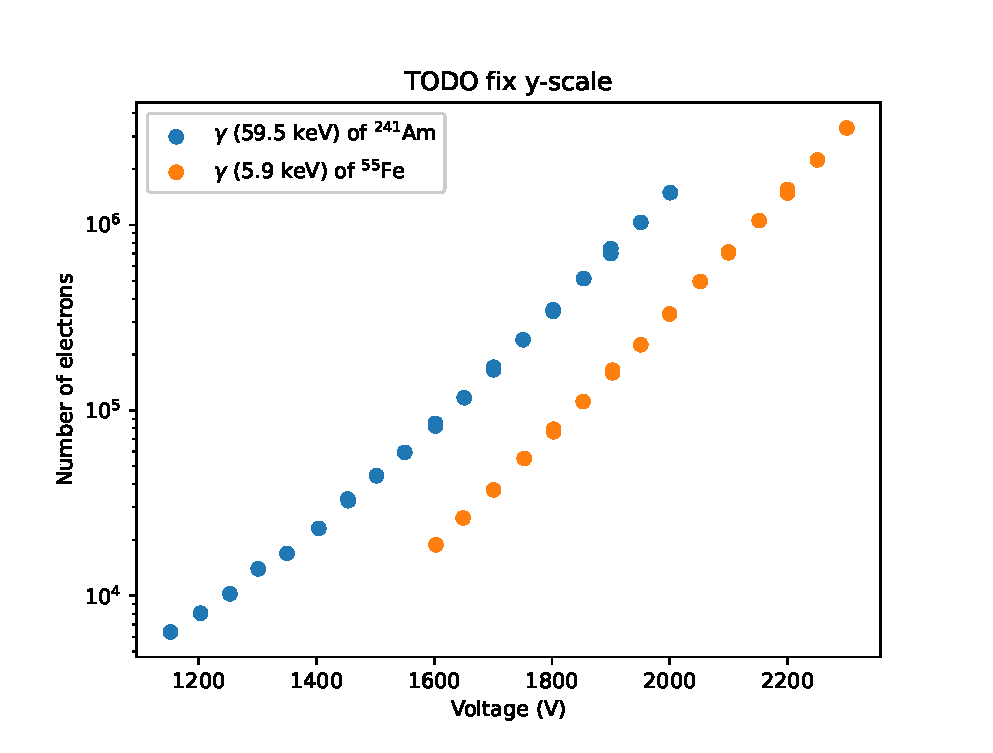
\includegraphics[width=\textwidth]{fig/python/hv_scans.eps}
\caption{Measured charge as a function of voltage}
\label{fig:hv_scans}
\end{figure}

\FloatBarrier
The measured charges were converted to gas multiplication factors with formula TODO, and the Diethorn formula was used to obtain theoretical predictions.
The anode and cathode radii and their uncertainties are provided in table \ref{table:sizes}, and air pressure was measured to be $1014 \pm 5$ mbar.
The results are plotted in figure \ref{fig:gas_mult}.
The results fit within the error limits of the theoretical predictions, but are consistently slightly higher.

\begin{figure}[ht!]
\centering
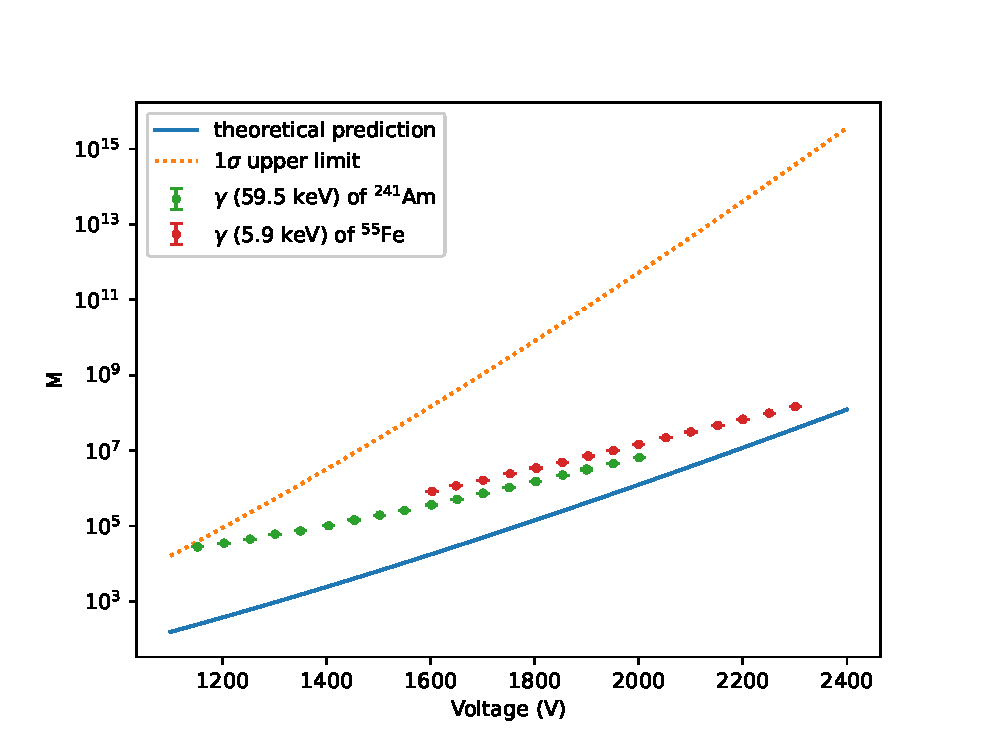
\includegraphics[width=\textwidth]{fig/python/gas_mult.eps}
\caption{Gas multiplication factor as a function of voltage}
\label{fig:gas_mult}
\end{figure}

\FloatBarrier
The resolution of the detector was also investigated by analyzing the peak width as a function of the operation voltage as in figure \ref{fig:resolution}.
For optimal resolution a small peak width is desired.
The ideal operation voltage for $^{241}$Am appears to be around 1530 V, whereas for $^{55}$Fe the peak width slightly decreases, as voltage is lowered beyond the suitable operation range.
Presumably this could mean that the ideal measurement voltage for $^{55}$Fe is in the same range as for $^{241}$Am, but improvements in the readout electronics are required for operation in this range.

\begin{figure}[ht!]
\centering
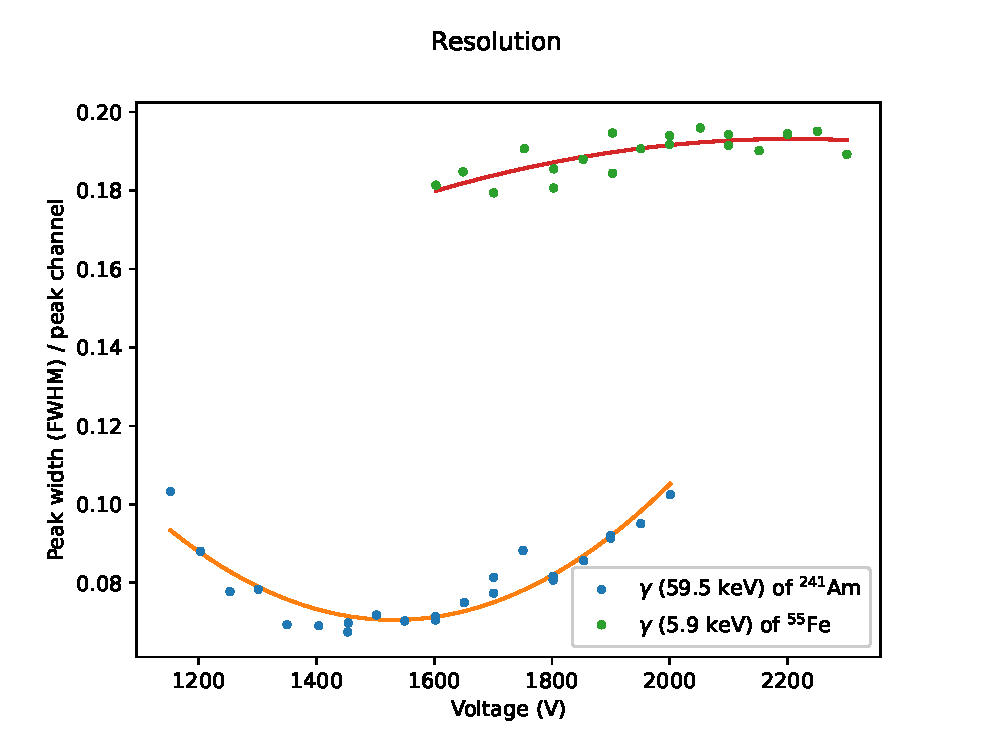
\includegraphics[width=\textwidth]{fig/python/resolution.eps}
\caption{Resolution as a function of voltage}
\label{fig:resolution}
\end{figure}

\FloatBarrier
Overall the results indicate that the detector is operating as intended, and its behaviour corresponds to the theoretical predictions.
They also provide some insights on the optimal operation conditions, but more measurements with different sources would be required to achieve conclusive results on the latter.



\clearpage
\subsection{Spectral measurement}
\label{results_spectral}
To obtain accurate spectral data, long spectral measurements were made with both sources, and without any source for determining the noise level.
The $^{241}$Am source was measured for 30 min, the $^{55}$Fe source for 15 min and the noise for 60 min.
Figure \ref{fig:spectra} contains the noise-subtracted spectra.
The energy axis has been determined by fitting Gaussians to the primary peak of $^{241}$Am and the two peaks of the $^{55}$Fe spectrum, and using their means as reference points corresponding to their known emission energies.
This energy calibration is illustrated in figure \ref{fig:spectral_calibration}.

\begin{figure}[ht!]
\centering
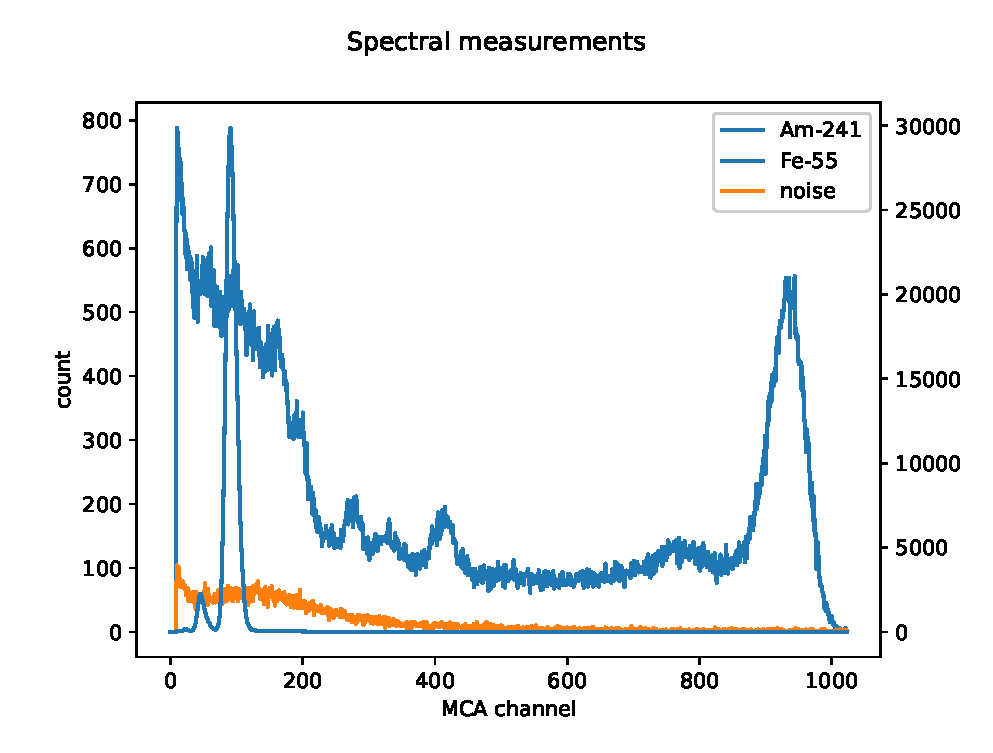
\includegraphics[width=\textwidth]{fig/python/spectra.eps}
\caption{Spectral measurements}
\label{fig:spectra}
\end{figure}

\begin{figure}[ht!]
\centering
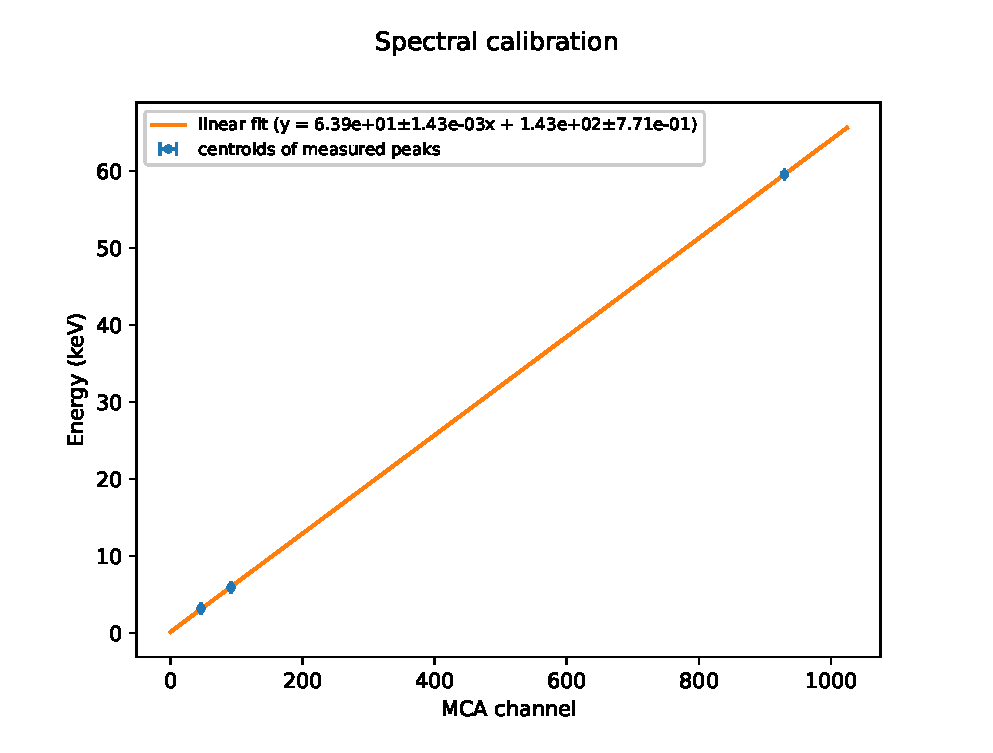
\includegraphics[width=\textwidth]{fig/python/spectral_calibration.eps}
\caption{Energy calibration with the spectral measurement}
\label{fig:spectral_calibration}
\end{figure}

\FloatBarrier
The secondary peak on the $^{55}$Fe spectrum is the Argon escape peak.
On the 

\begin{table}[ht!]
\centering
\caption{Measured spectral peaks}
\begin{tabular}{lllll}
Source	& MCA ch.	& $E_\text{est.}$ (keV)	& $E_\text{theor.}$ (keV)	& Origin \\
\hline
$^{55}$Fe	& 46.22			& -			& 3.19 			& Argon escape peak \cite{winkler_gaseous_2015} \\
$^{55}$Fe	& 91.60			& -			& 5.90 			& $^{55}$Fe electron capture \cite{winkler_gaseous_2015} \\
$^{241}$Am	& 276.88			& 17.84		& 17.751			& $^{237}$Np L$_\beta$ \cites{maeda_peak_2015}{am241_spectrum} \\
$^{241}$Am	& 330.28			& 21.25		& 20.784			& $^{237}$Np L$_\gamma$ \cites{maeda_peak_2015}{am241_spectrum} \\
$^{241}$Am	& 412.10			& 26.48		& 26			& $^{241}$Am \cite{am241_spectrum} \\
$^{241}$Am	& 771.82			& 49.47		&				& \\
$^{241}$Am	& 929.26			& -			& 59.5409		& Byproduct of $\alpha$-decay \cite{winkler_gaseous_2015} \\
\end{tabular}
\end{table}




\clearpage
\section{Conclusions}
\label{conclusions}

The detector works as intended, and has shown its capability of distinguishing the energies of new spectral peaks accurately.
Therefore it is shown to be suitable for its intended purpose of being a cost-effective alternative for existing detectors.
However, in the measurements of appendix \ref{pre_amp} the detector showed unexpected degradation, which casts doubt on its long-term stability.
Additionally more error sources could be included in the error analysis, as at present the error bars are much tighter than the variations seen in the results.


\clearpage
\begin{appendices}

\section{Pre-amplifier}
\label{pre_amp}
A custom pre-amplifier was constructed to serve as a replacement for the commercial pre-amplifier used in the measurements of section \ref{results}.
This pre-amplifier required a custom power supply, as the operational amplifier used in the pre-amplifier requires supplies of both positive and negative voltage of 5 V.
The first step was to test the power supply components on a breadboard, as in figure \ref{fig:pre_amp_psu_testing}.
Once it was verified that the components worked, they were soldered on a PCB, resulting in the device in figure \ref{fig:pre_amp_psu}

\begin{figure}[ht!]
\centering
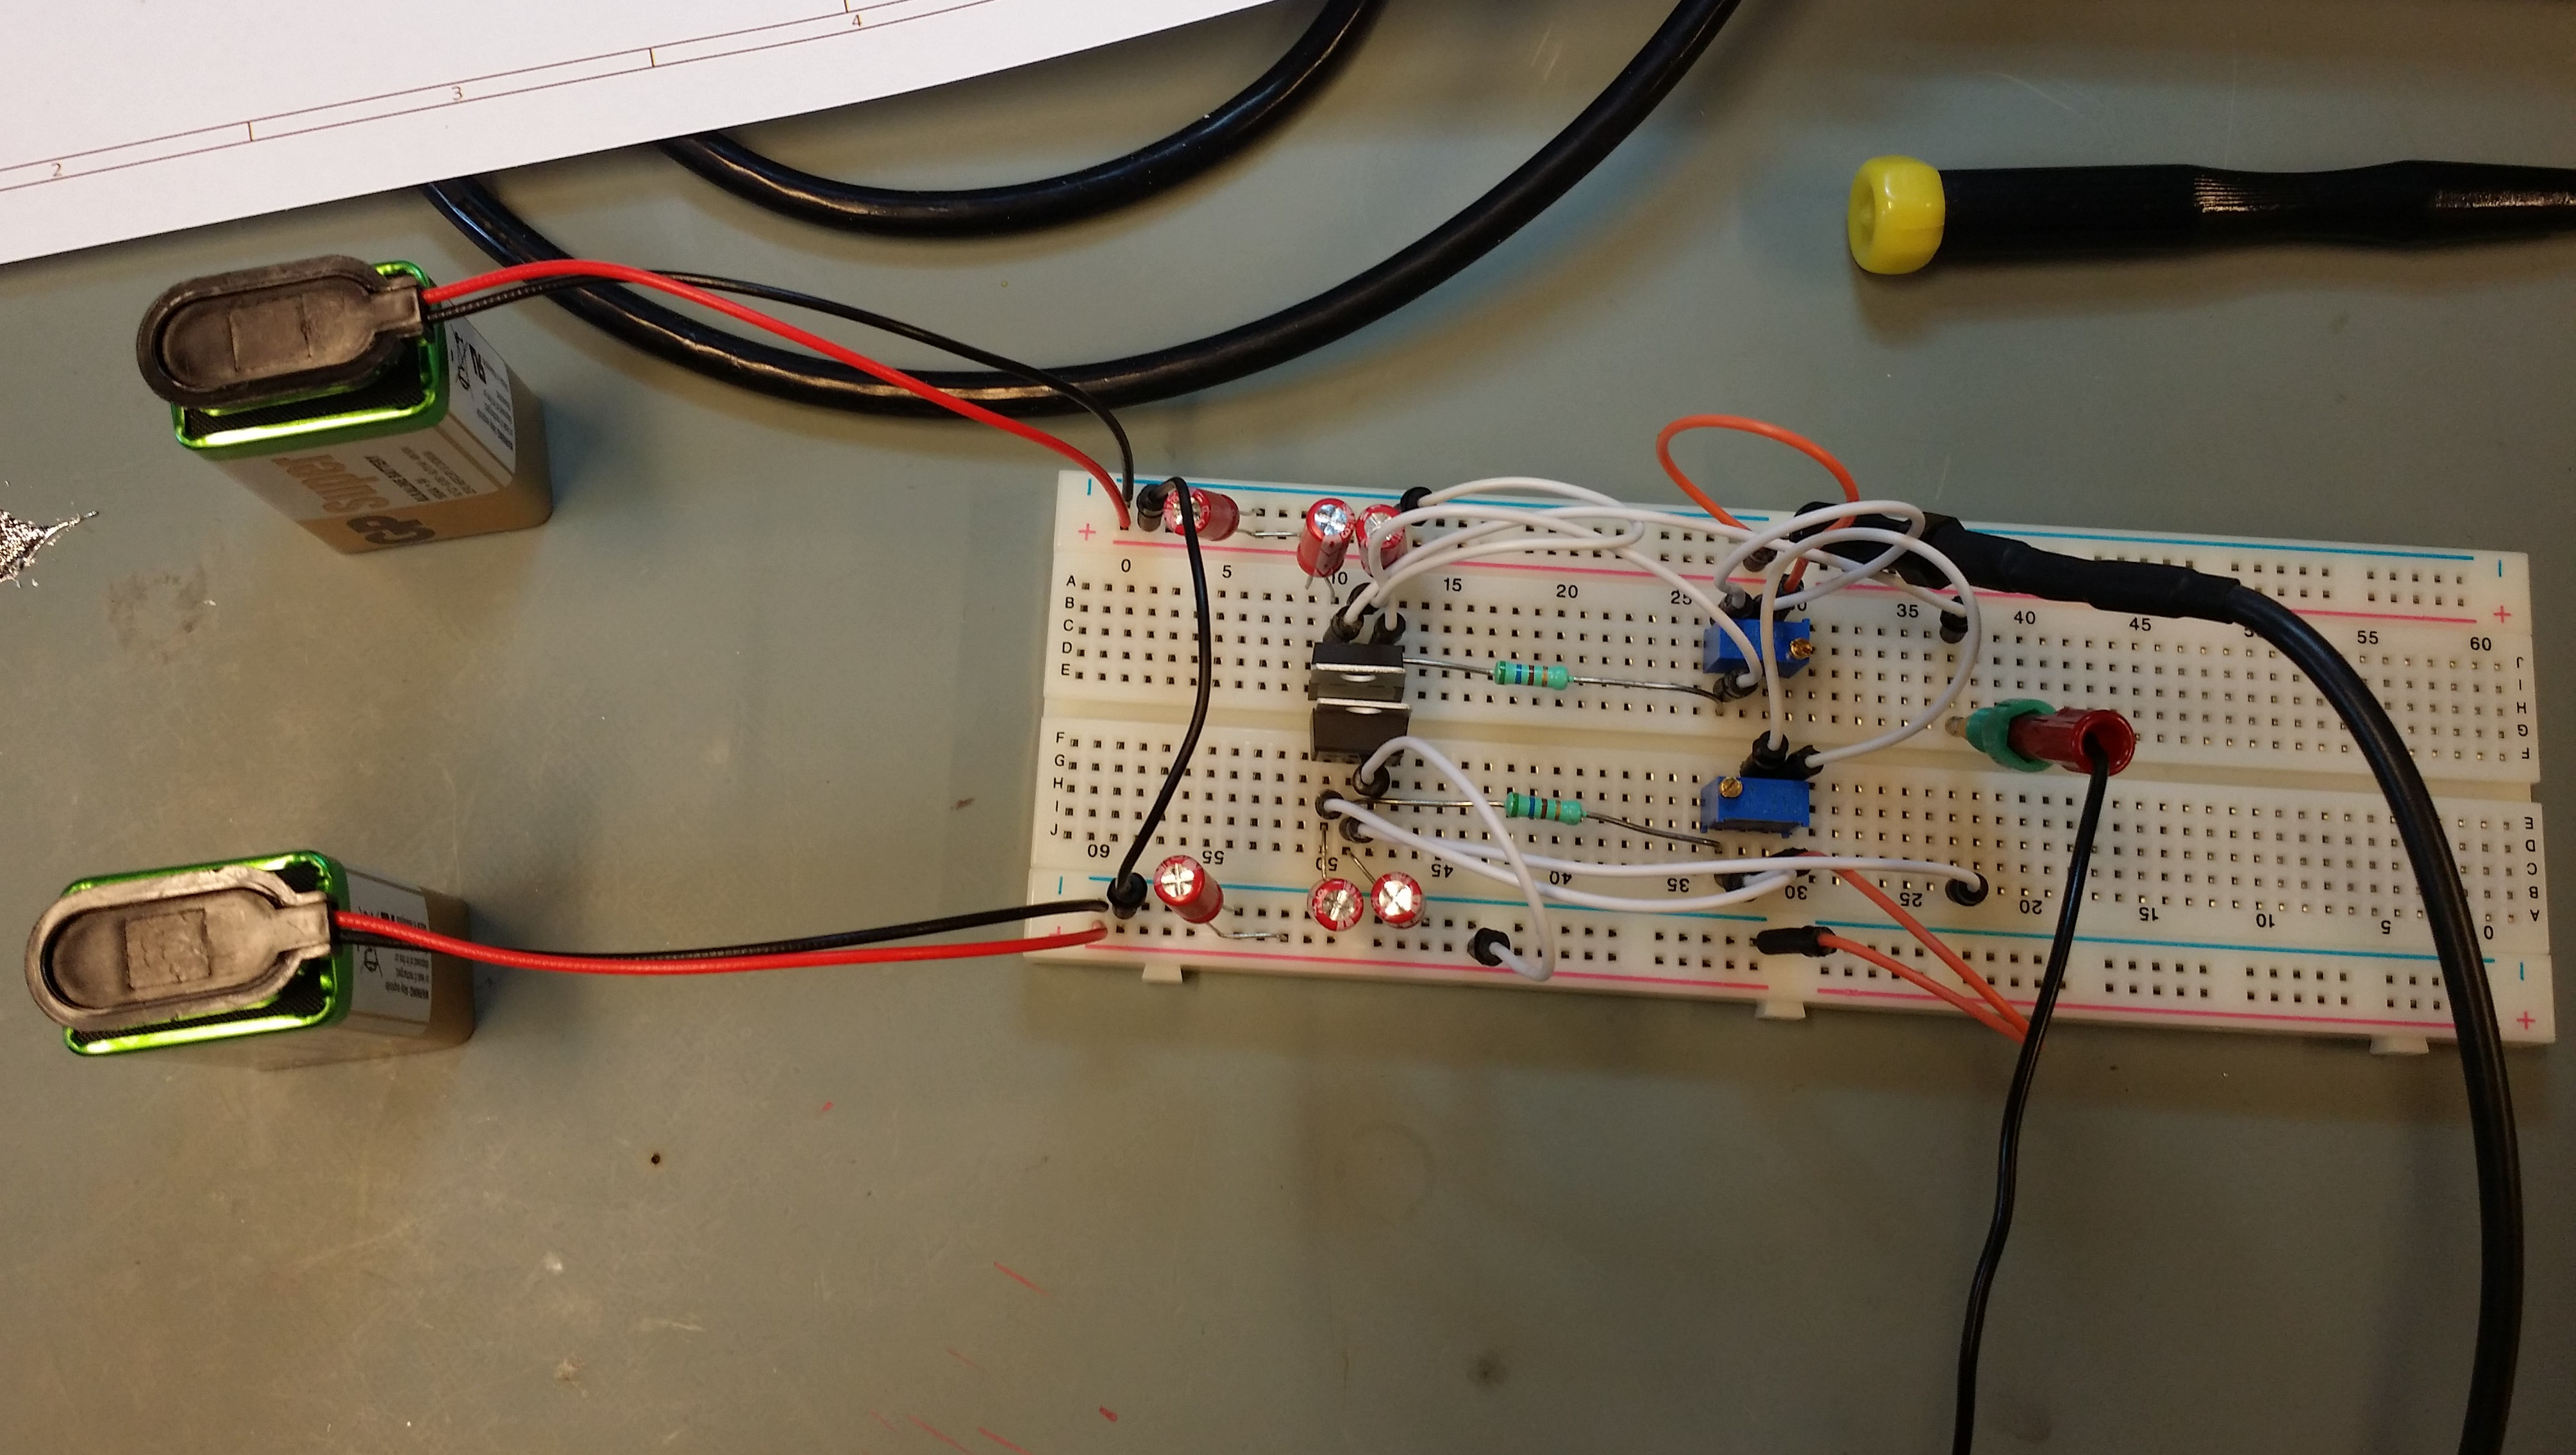
\includegraphics[width=\textwidth]{fig/IMG_20201005_104331-cropped.jpg}
\caption{Preliminary testing of the components of the pre-amplifier power supply}
\label{fig:pre_amp_psu_testing}
\end{figure}

\begin{figure}[ht!]
\centering
\begin{subfigure}[t]{0.48\textwidth}
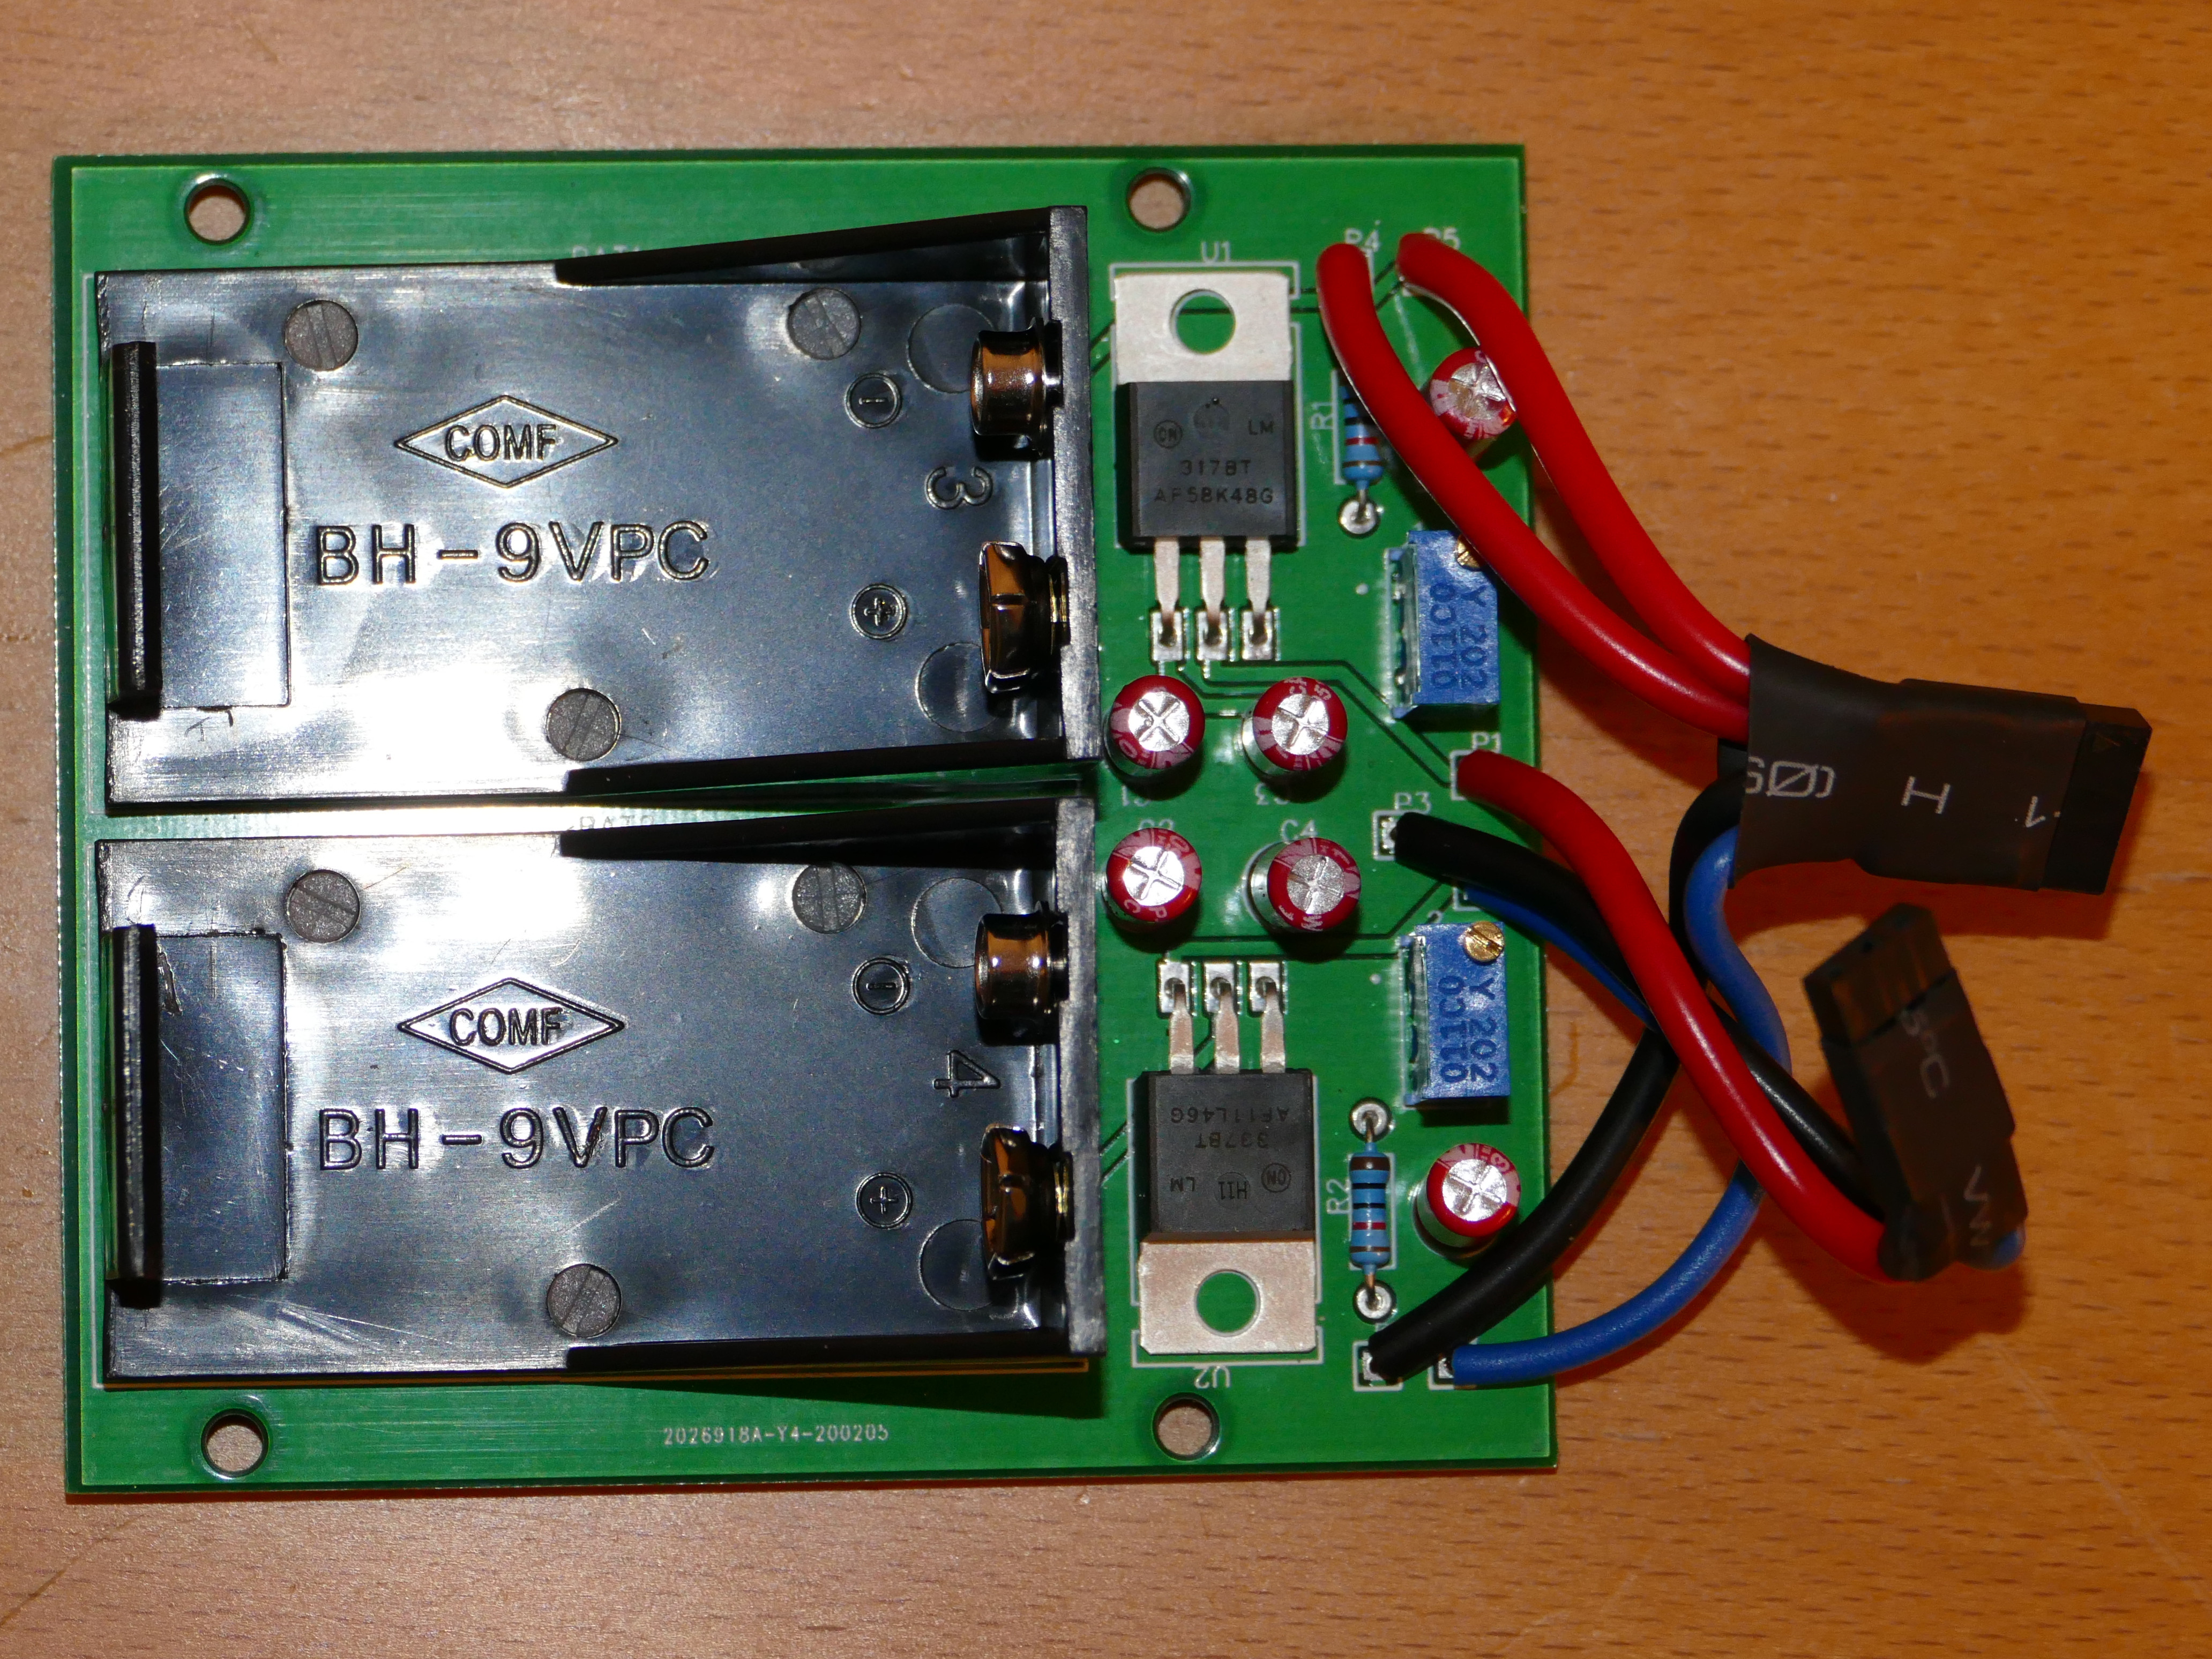
\includegraphics[width=\textwidth]{fig/P1170891-cropped.jpg}
\end{subfigure}
%
\begin{subfigure}[t]{0.48\textwidth}
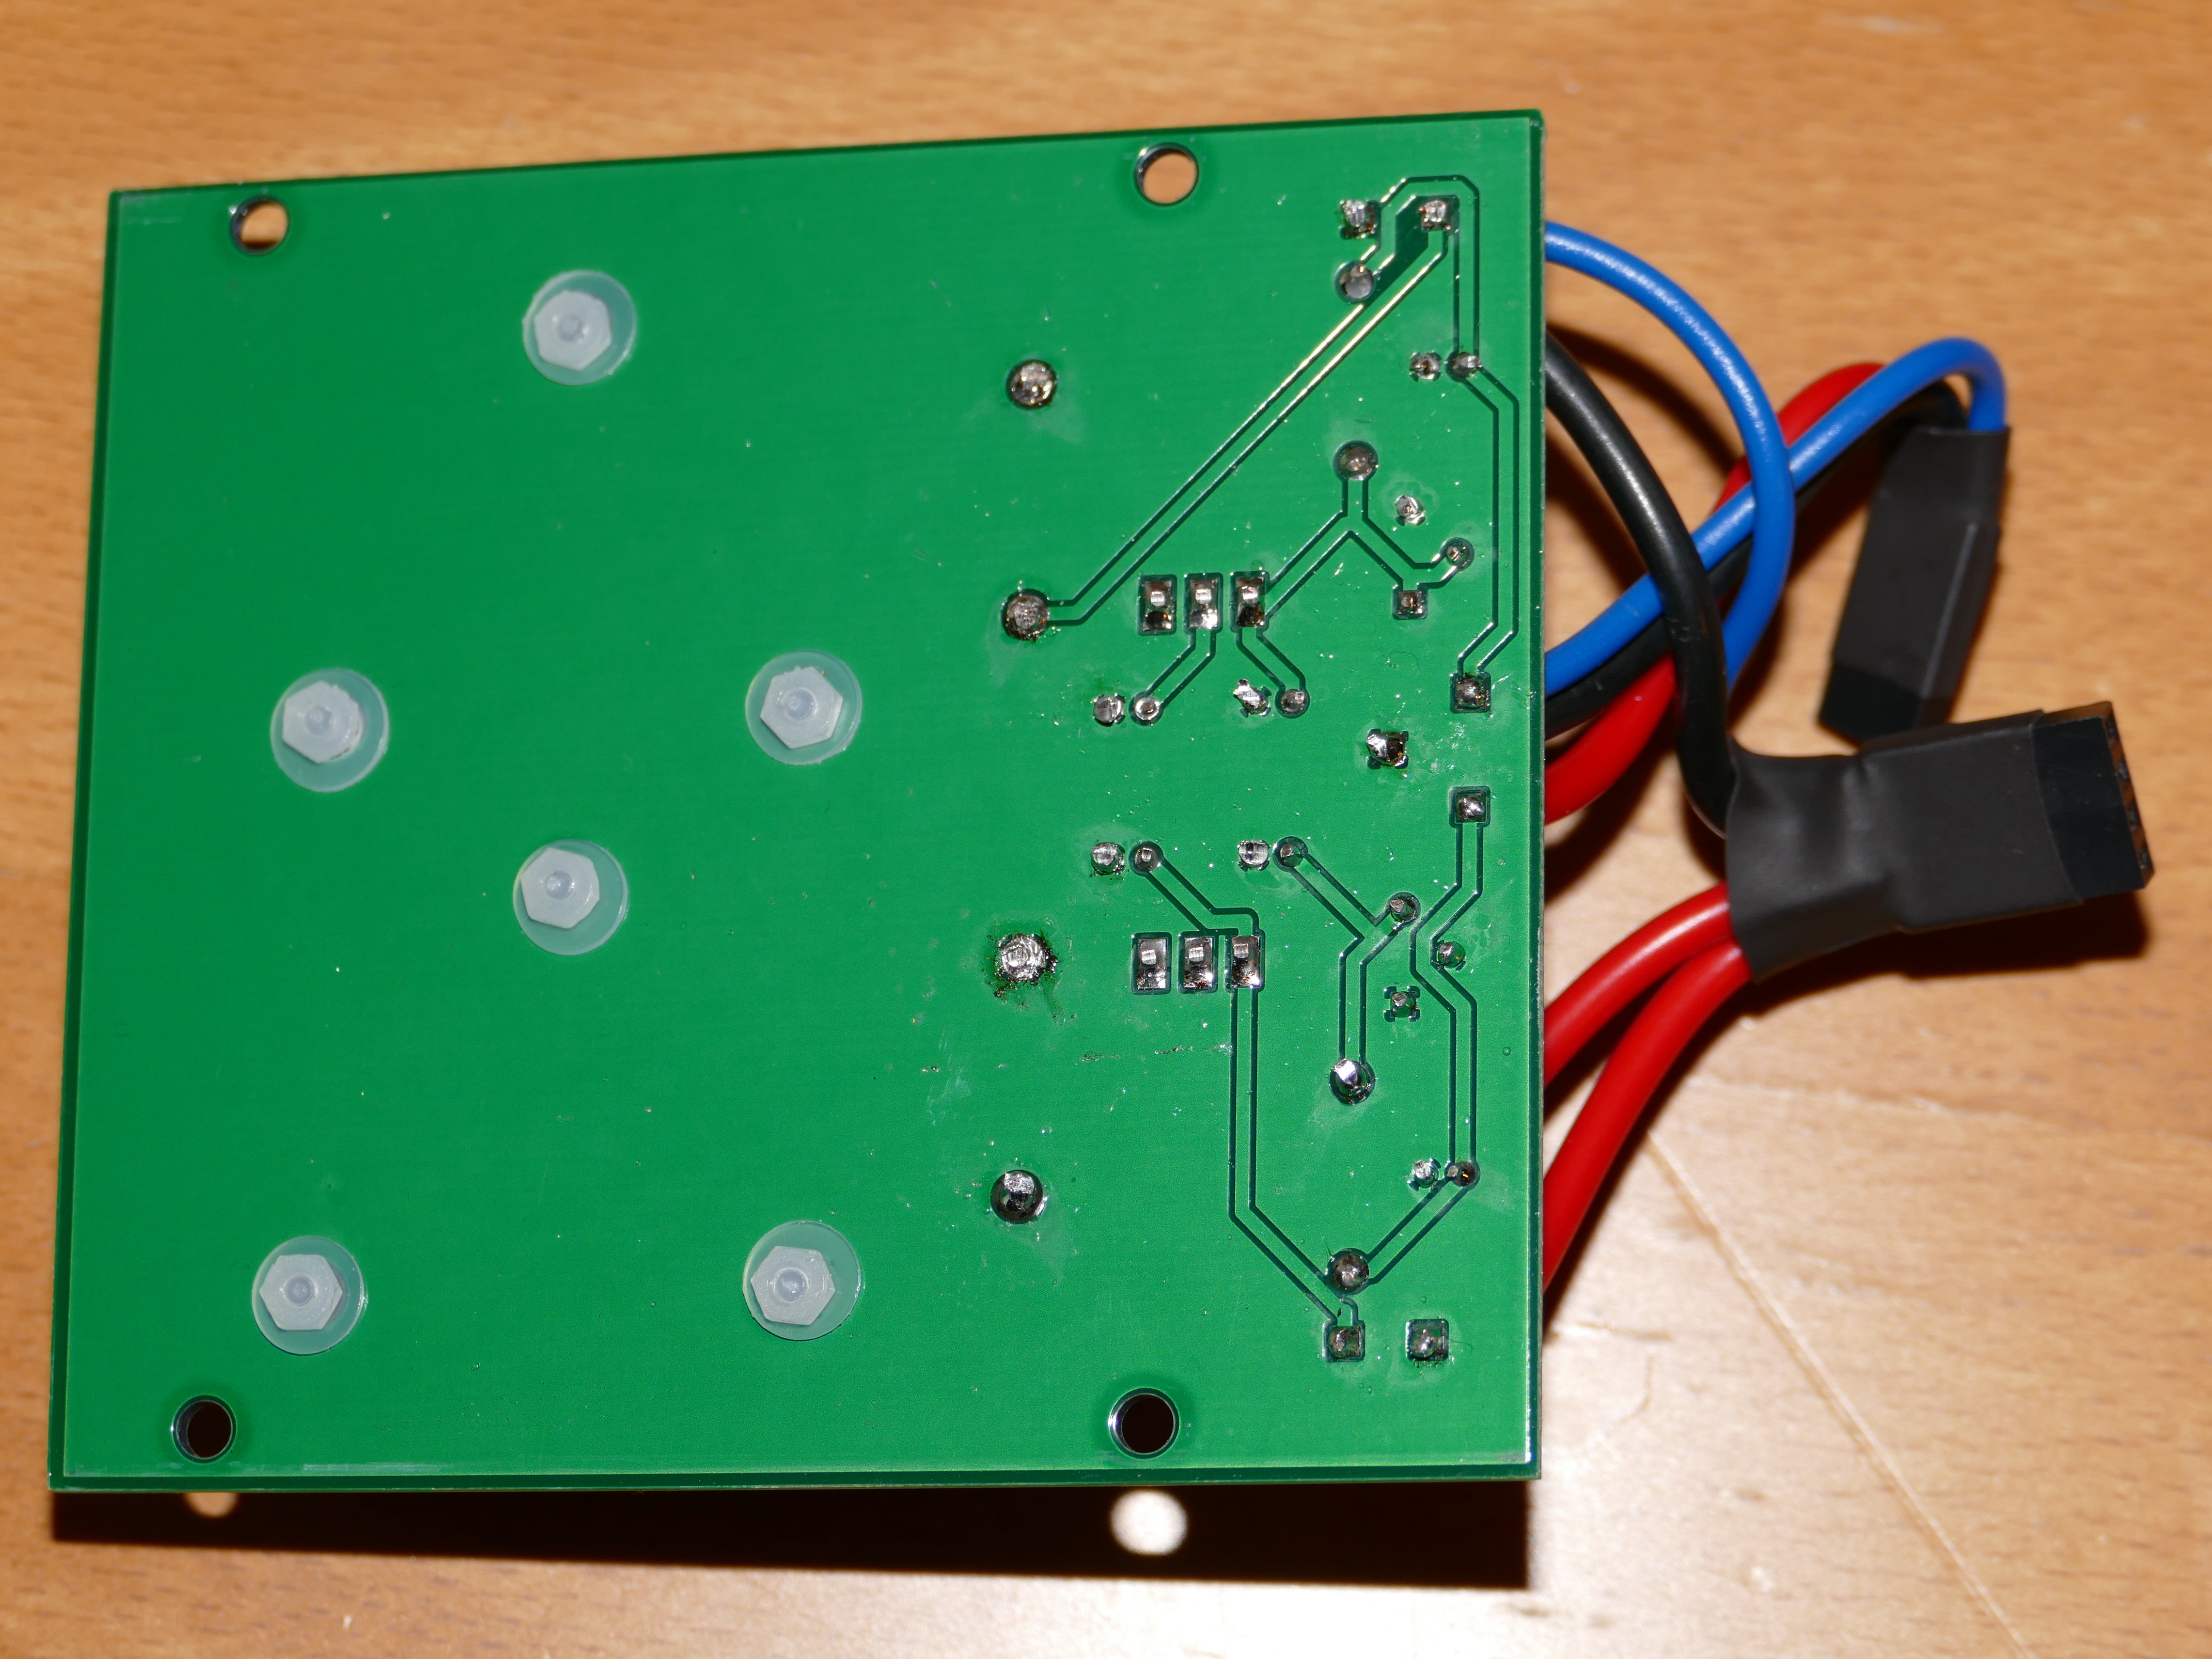
\includegraphics[width=\textwidth]{fig/P1170894-cropped.jpg}
\end{subfigure}
%
\caption{Power supply for the pre-amplifier}
\label{fig:pre_amp_psu}
\end{figure}

\FloatBarrier
The pre-amplifier itself was assembled on another PCB according to the schematic in figure \ref{fig:pre_amp_schematic}.
Its core is the
\href{https://www.ti.com/product/OPA657}{Texas Instruments OPA657}
\href{https://en.wikipedia.org/wiki/Operational_amplifier}{operational amplifier},
and the values for the various resistors and capacitors have been set according to its specifications to achieve the gain value $G = 21$.
The assembled pre-amplifier is shown in figure \ref{fig:pre_amp_board}, and its mounting is illustrated in figure \ref{fig:pre_amp_mounting}.
We also built a switch panel of figure \ref{fig:pre_amp_switch} for the power supply.
The final assembled pre-amplifier is shown in figure \ref{fig:pre_amp}.


\begin{figure}[ht!]
\centering
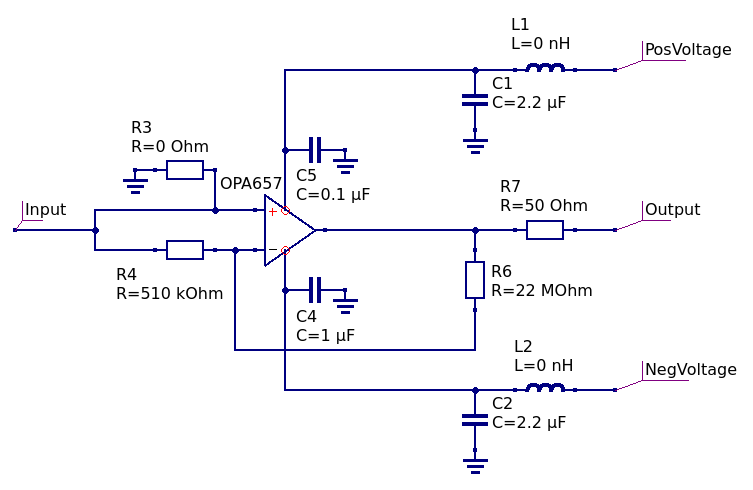
\includegraphics[width=\textwidth]{fig/amp-schematic/amplifier.png}
\caption{Circuit diagram of the pre-amplifier}
\label{fig:pre_amp_schematic}
\end{figure}

\begin{figure}[ht!]
\centering
% 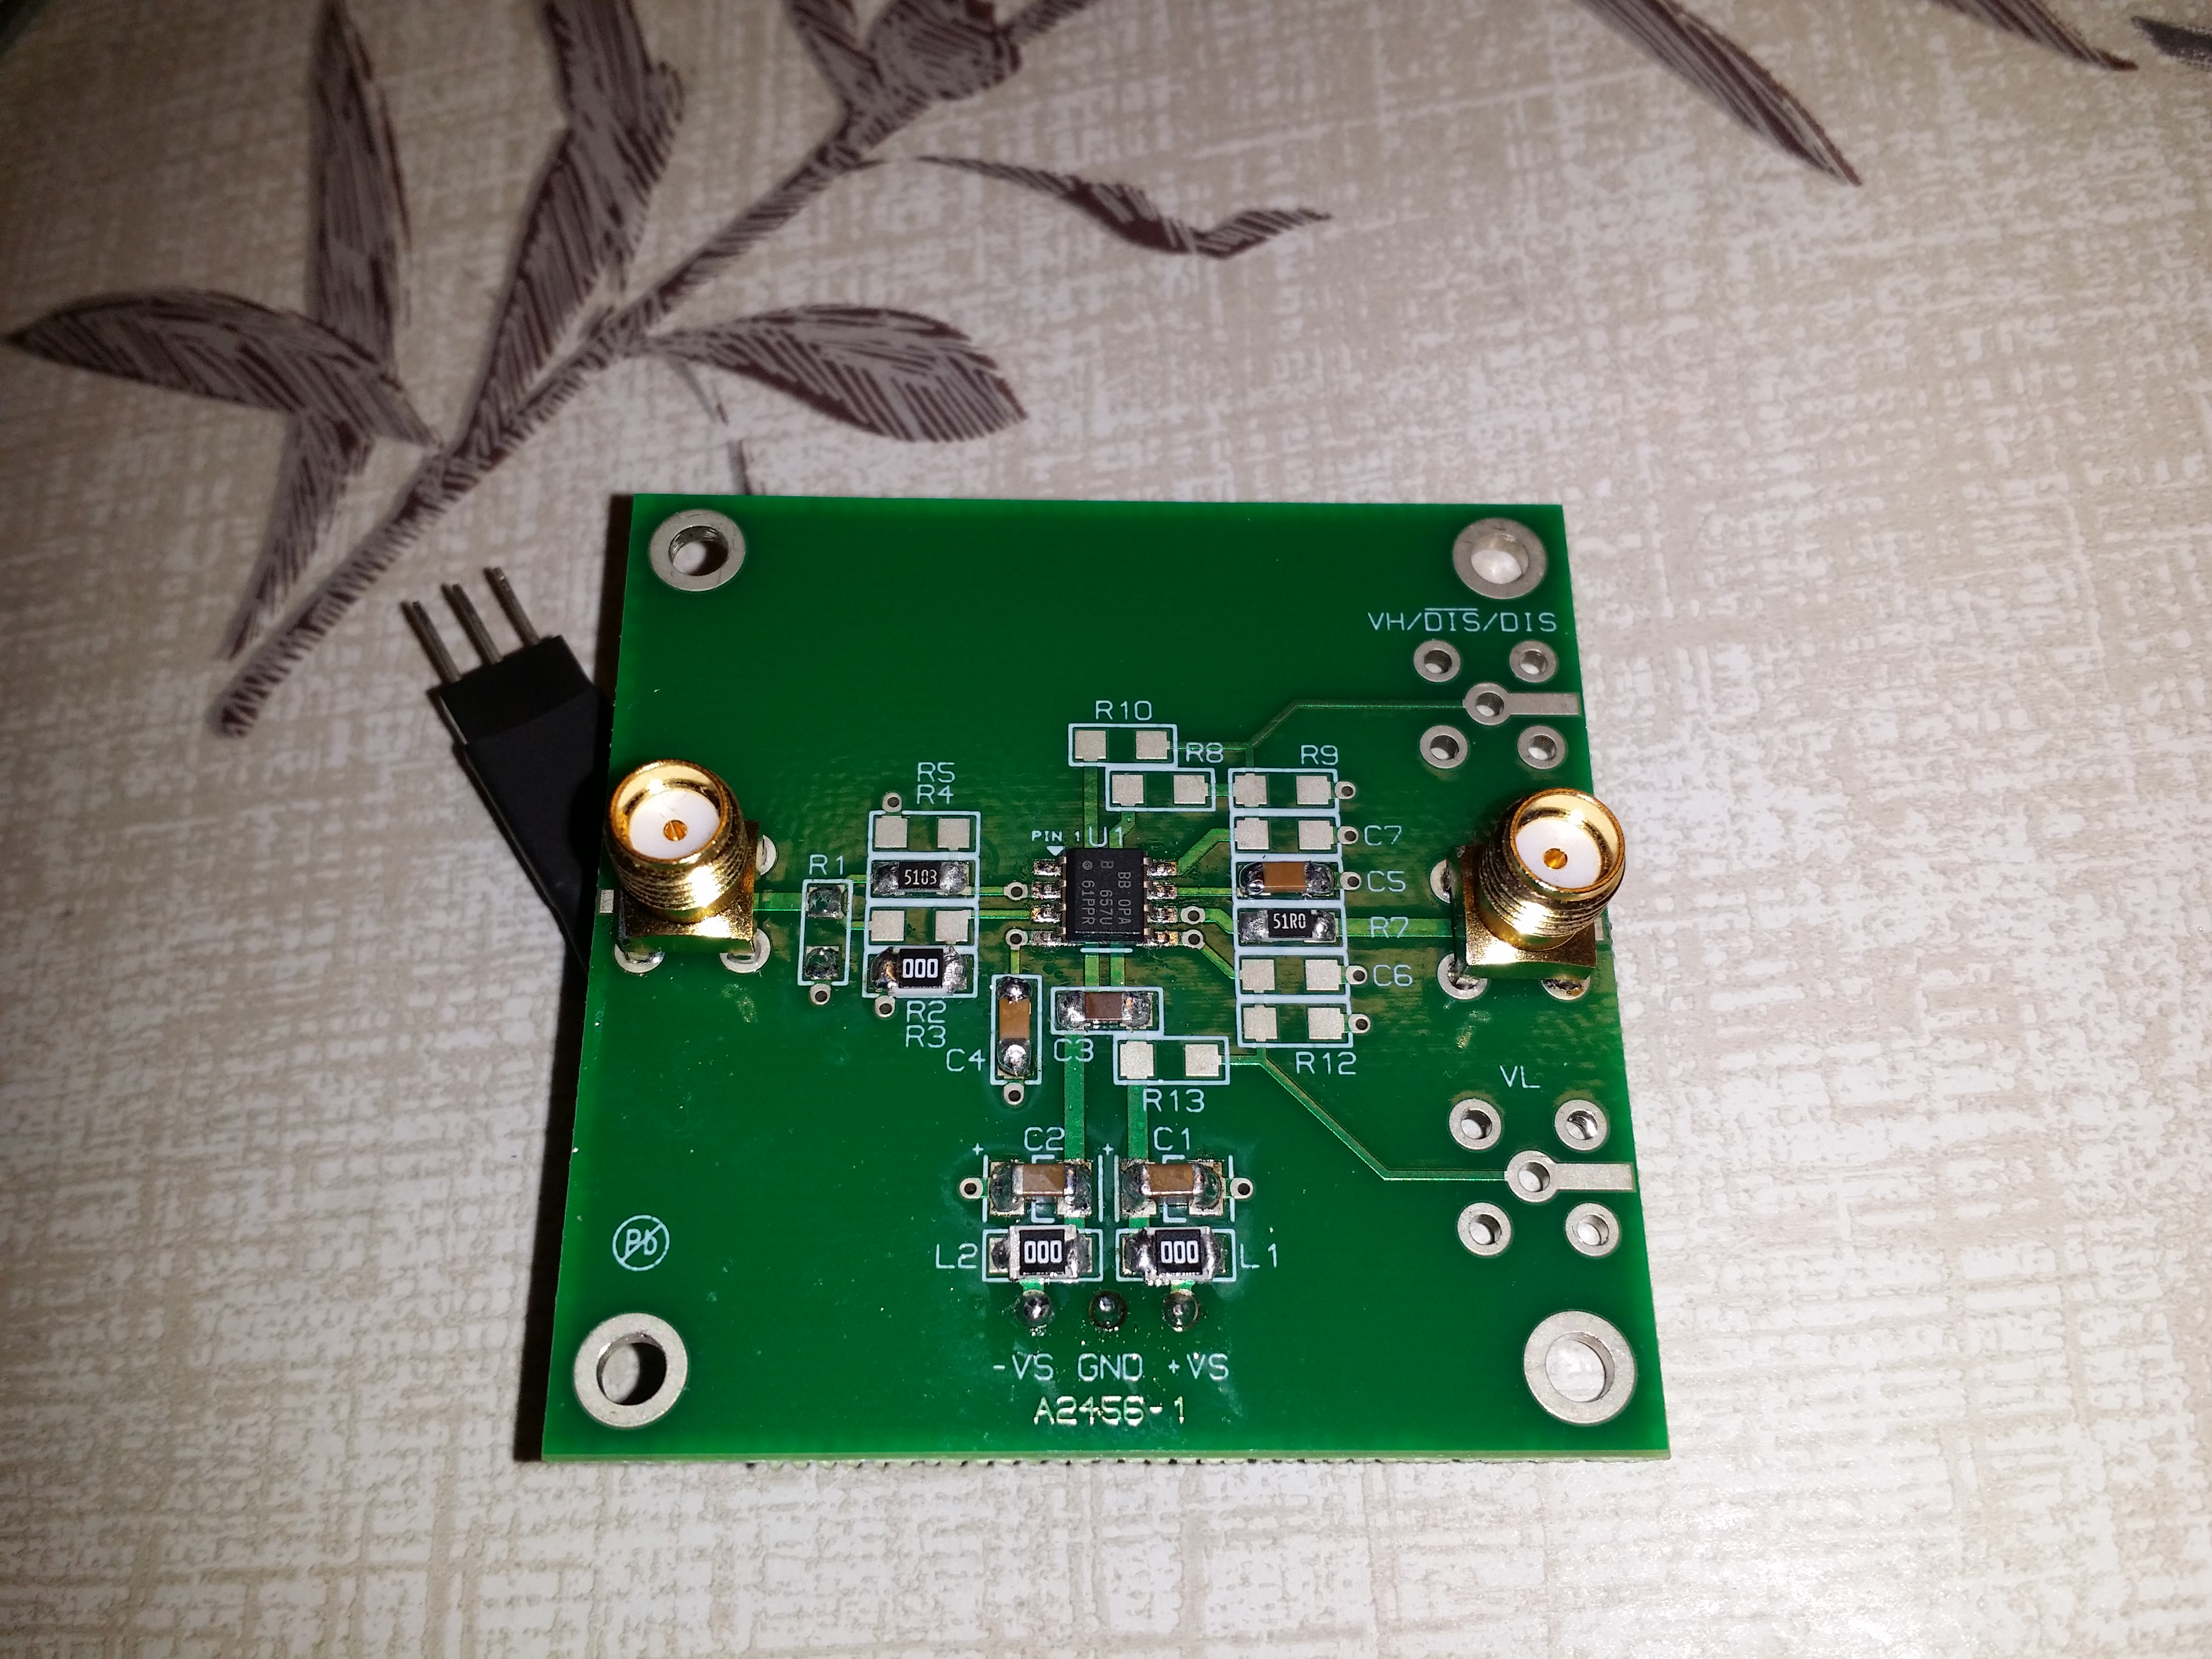
\includegraphics[width=\textwidth]{fig/IMG_20201207_121010.jpg}
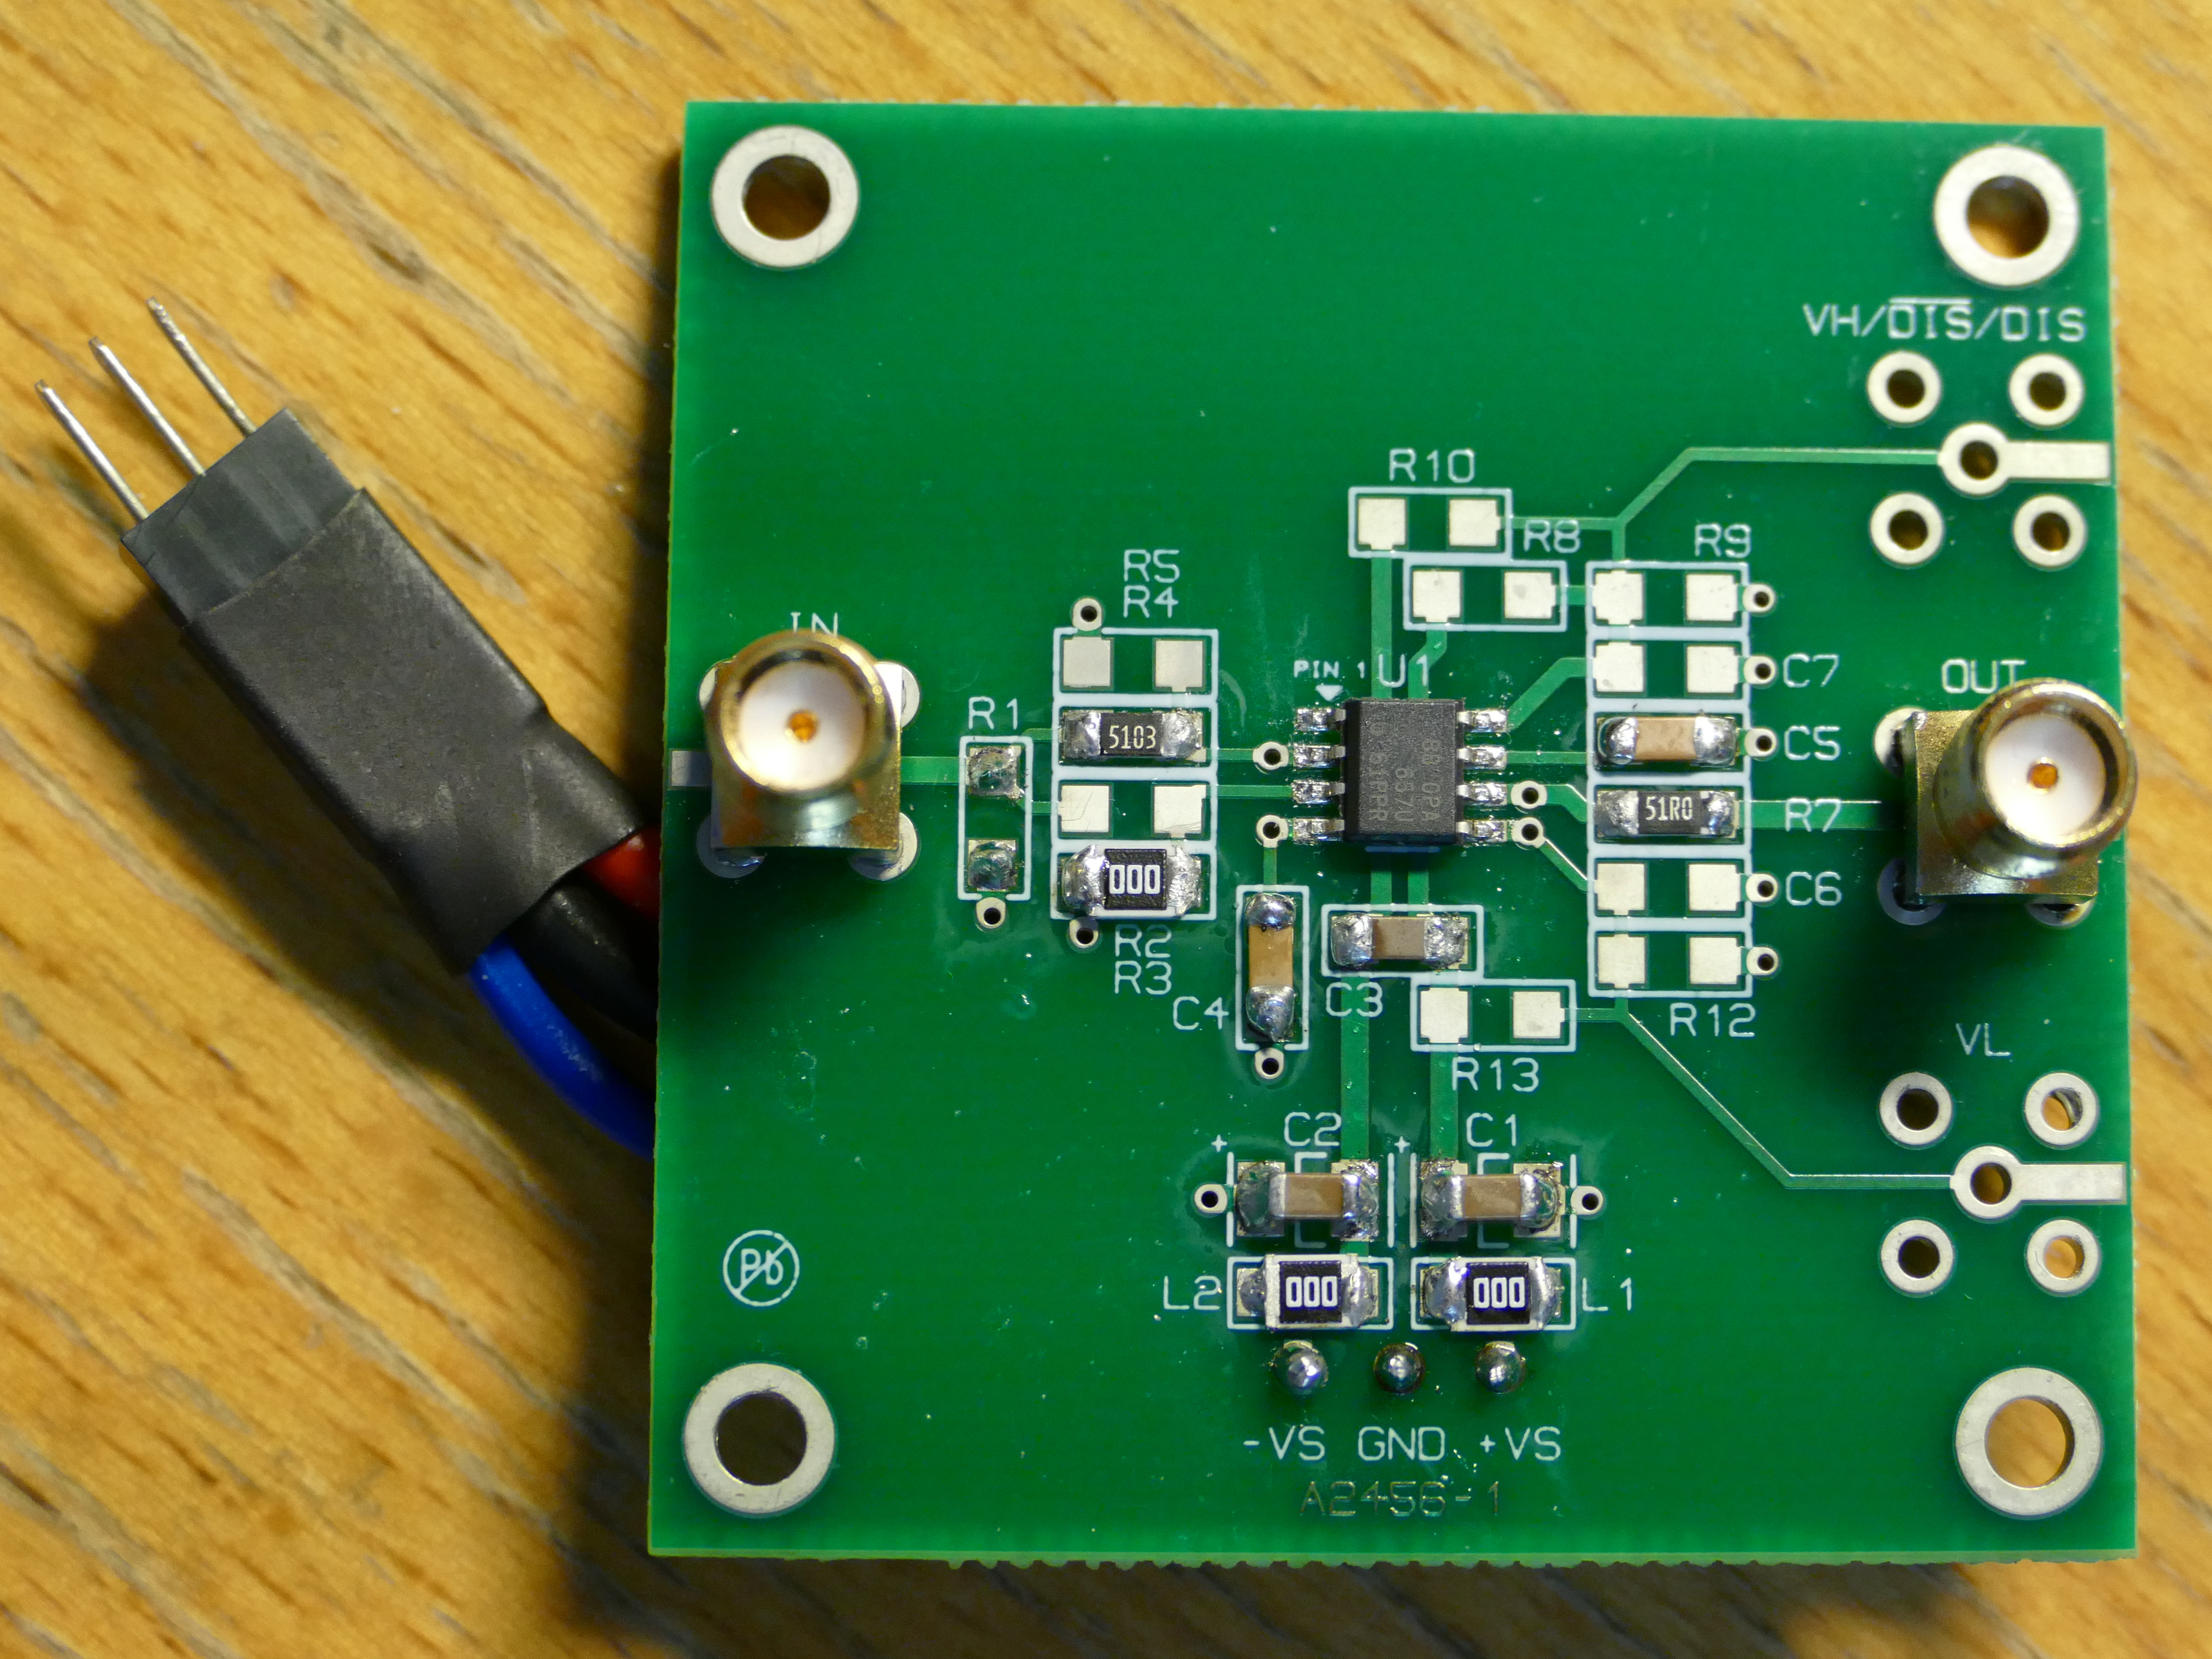
\includegraphics[width=0.9\textwidth]{fig/P1170917-cropped.jpg}
\caption{Pre-amplifier board}
\label{fig:pre_amp_board}
\end{figure}

\begin{figure}[ht!]
\centering
\begin{subfigure}[t]{0.48\textwidth}
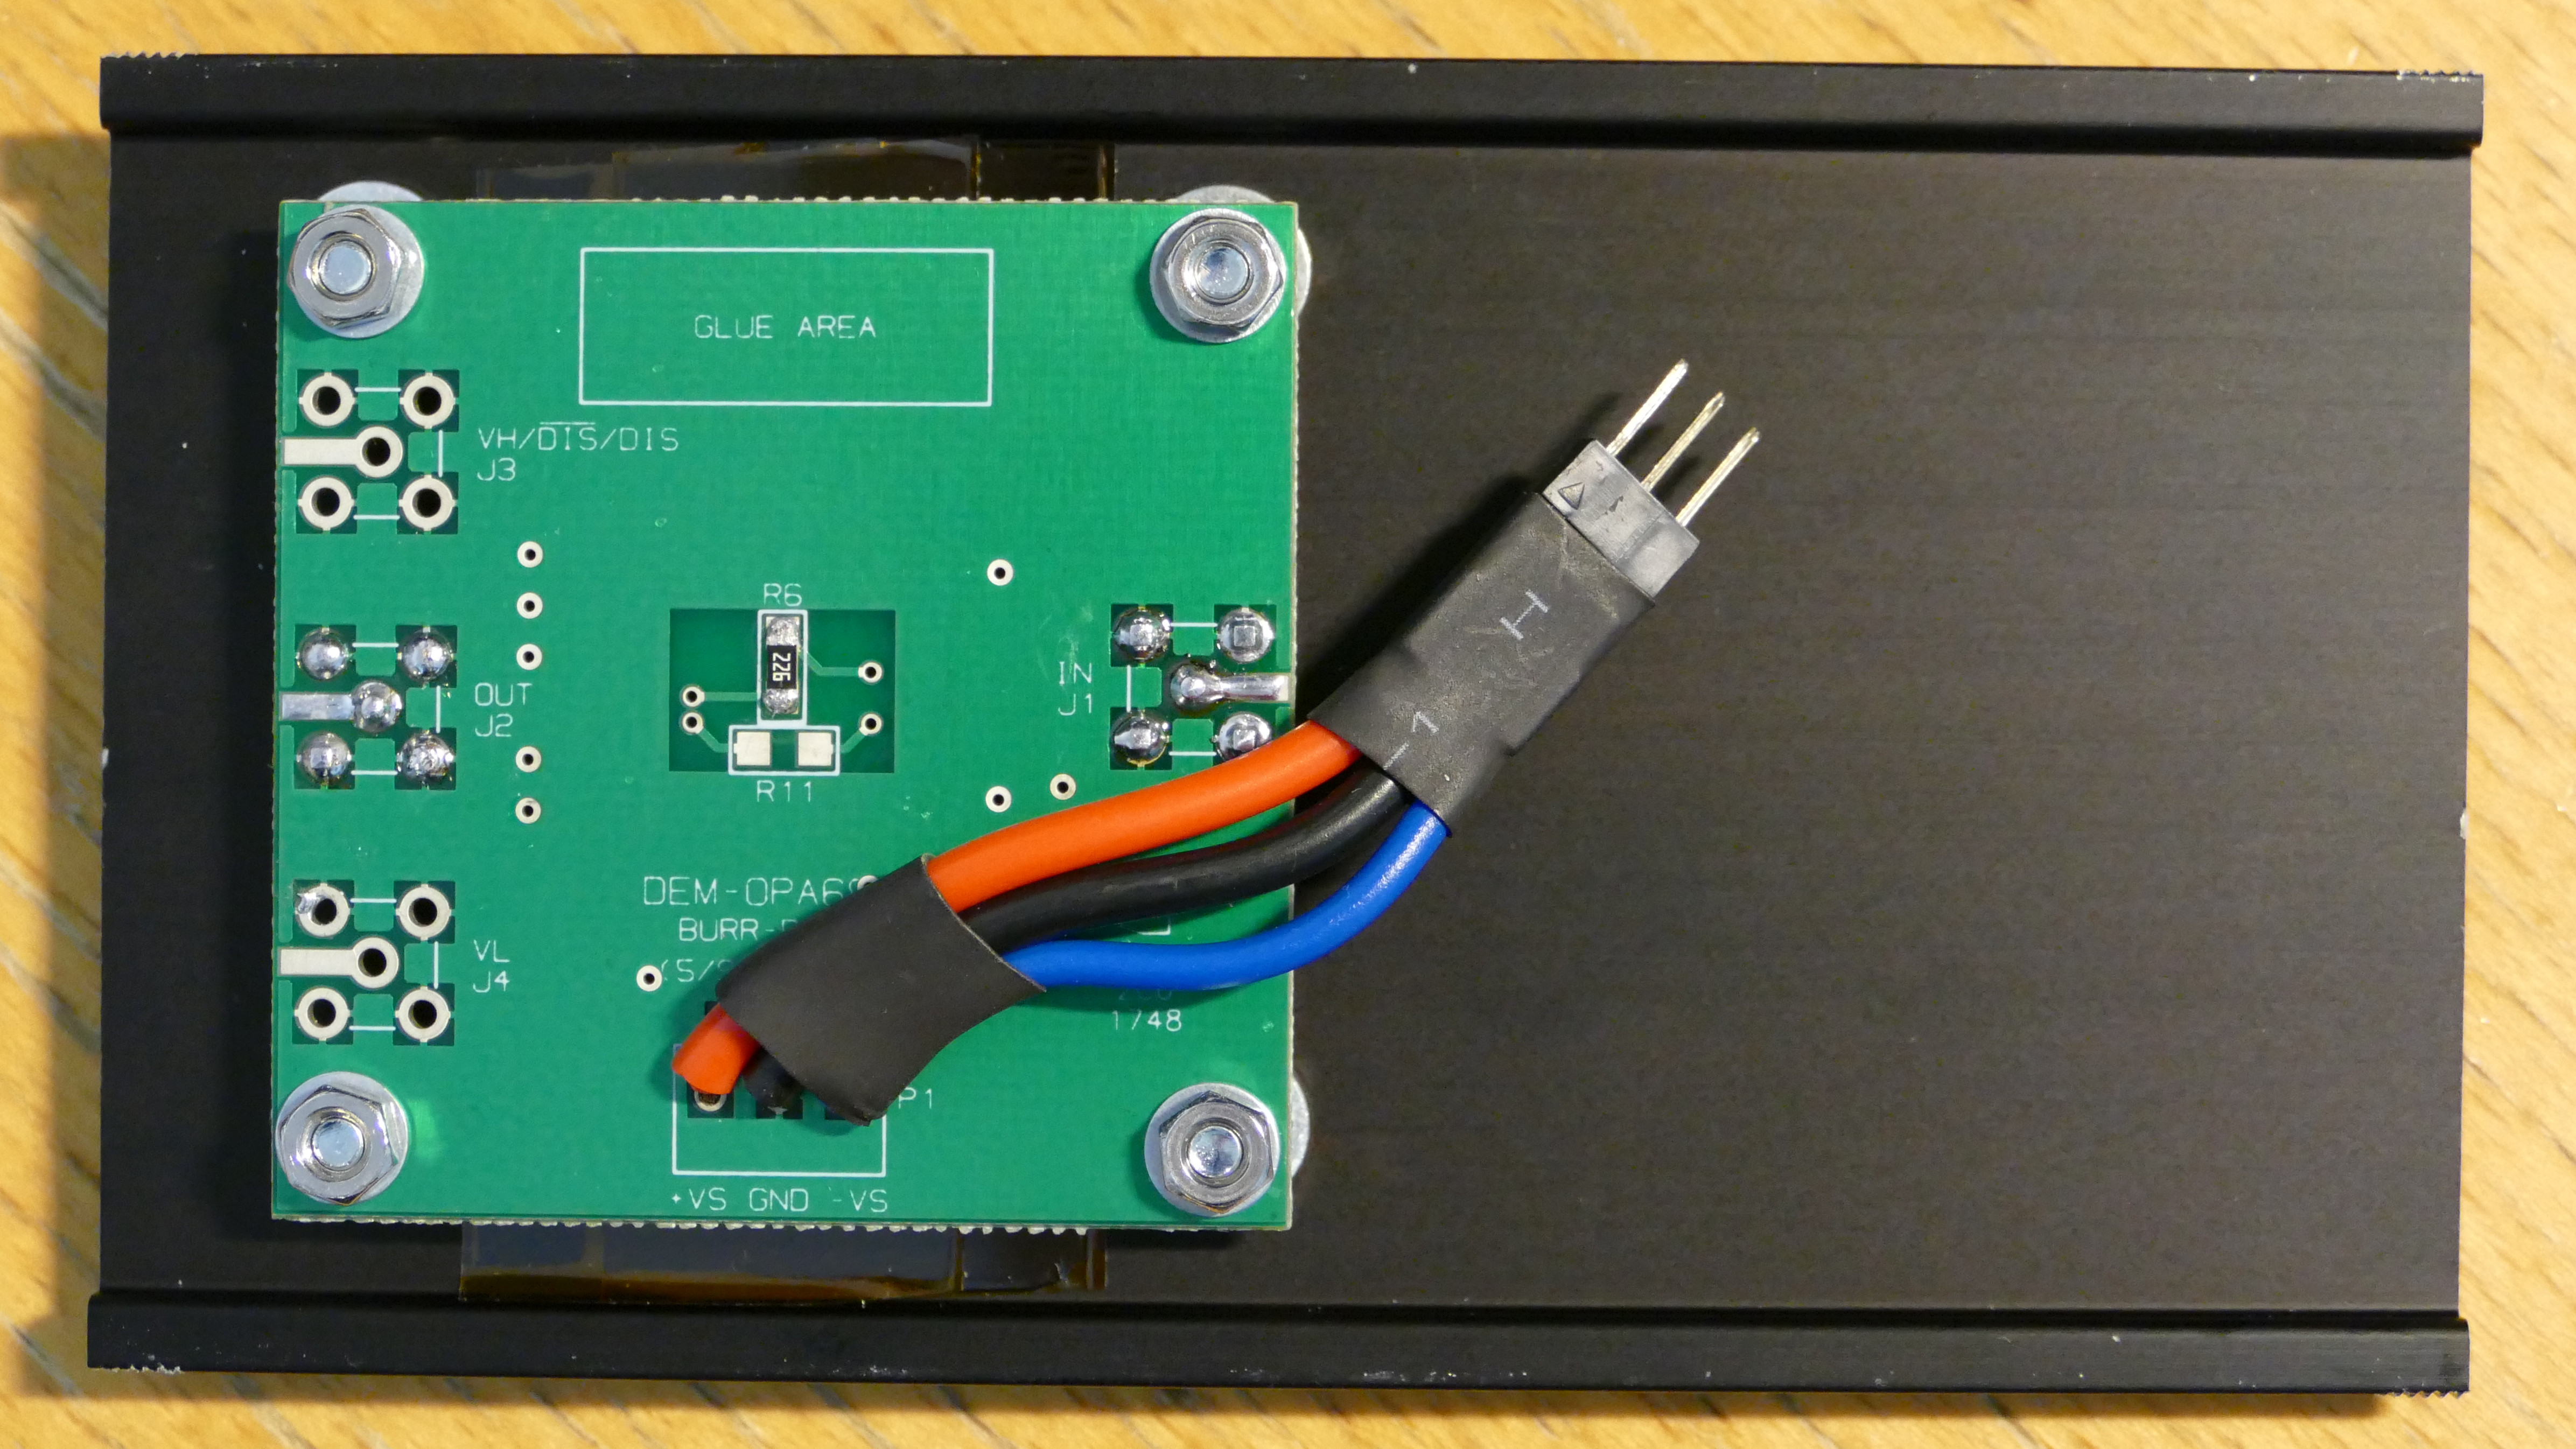
\includegraphics[width=\textwidth]{fig/P1170915-cropped.jpg}
\end{subfigure}
%
\begin{subfigure}[t]{0.48\textwidth}
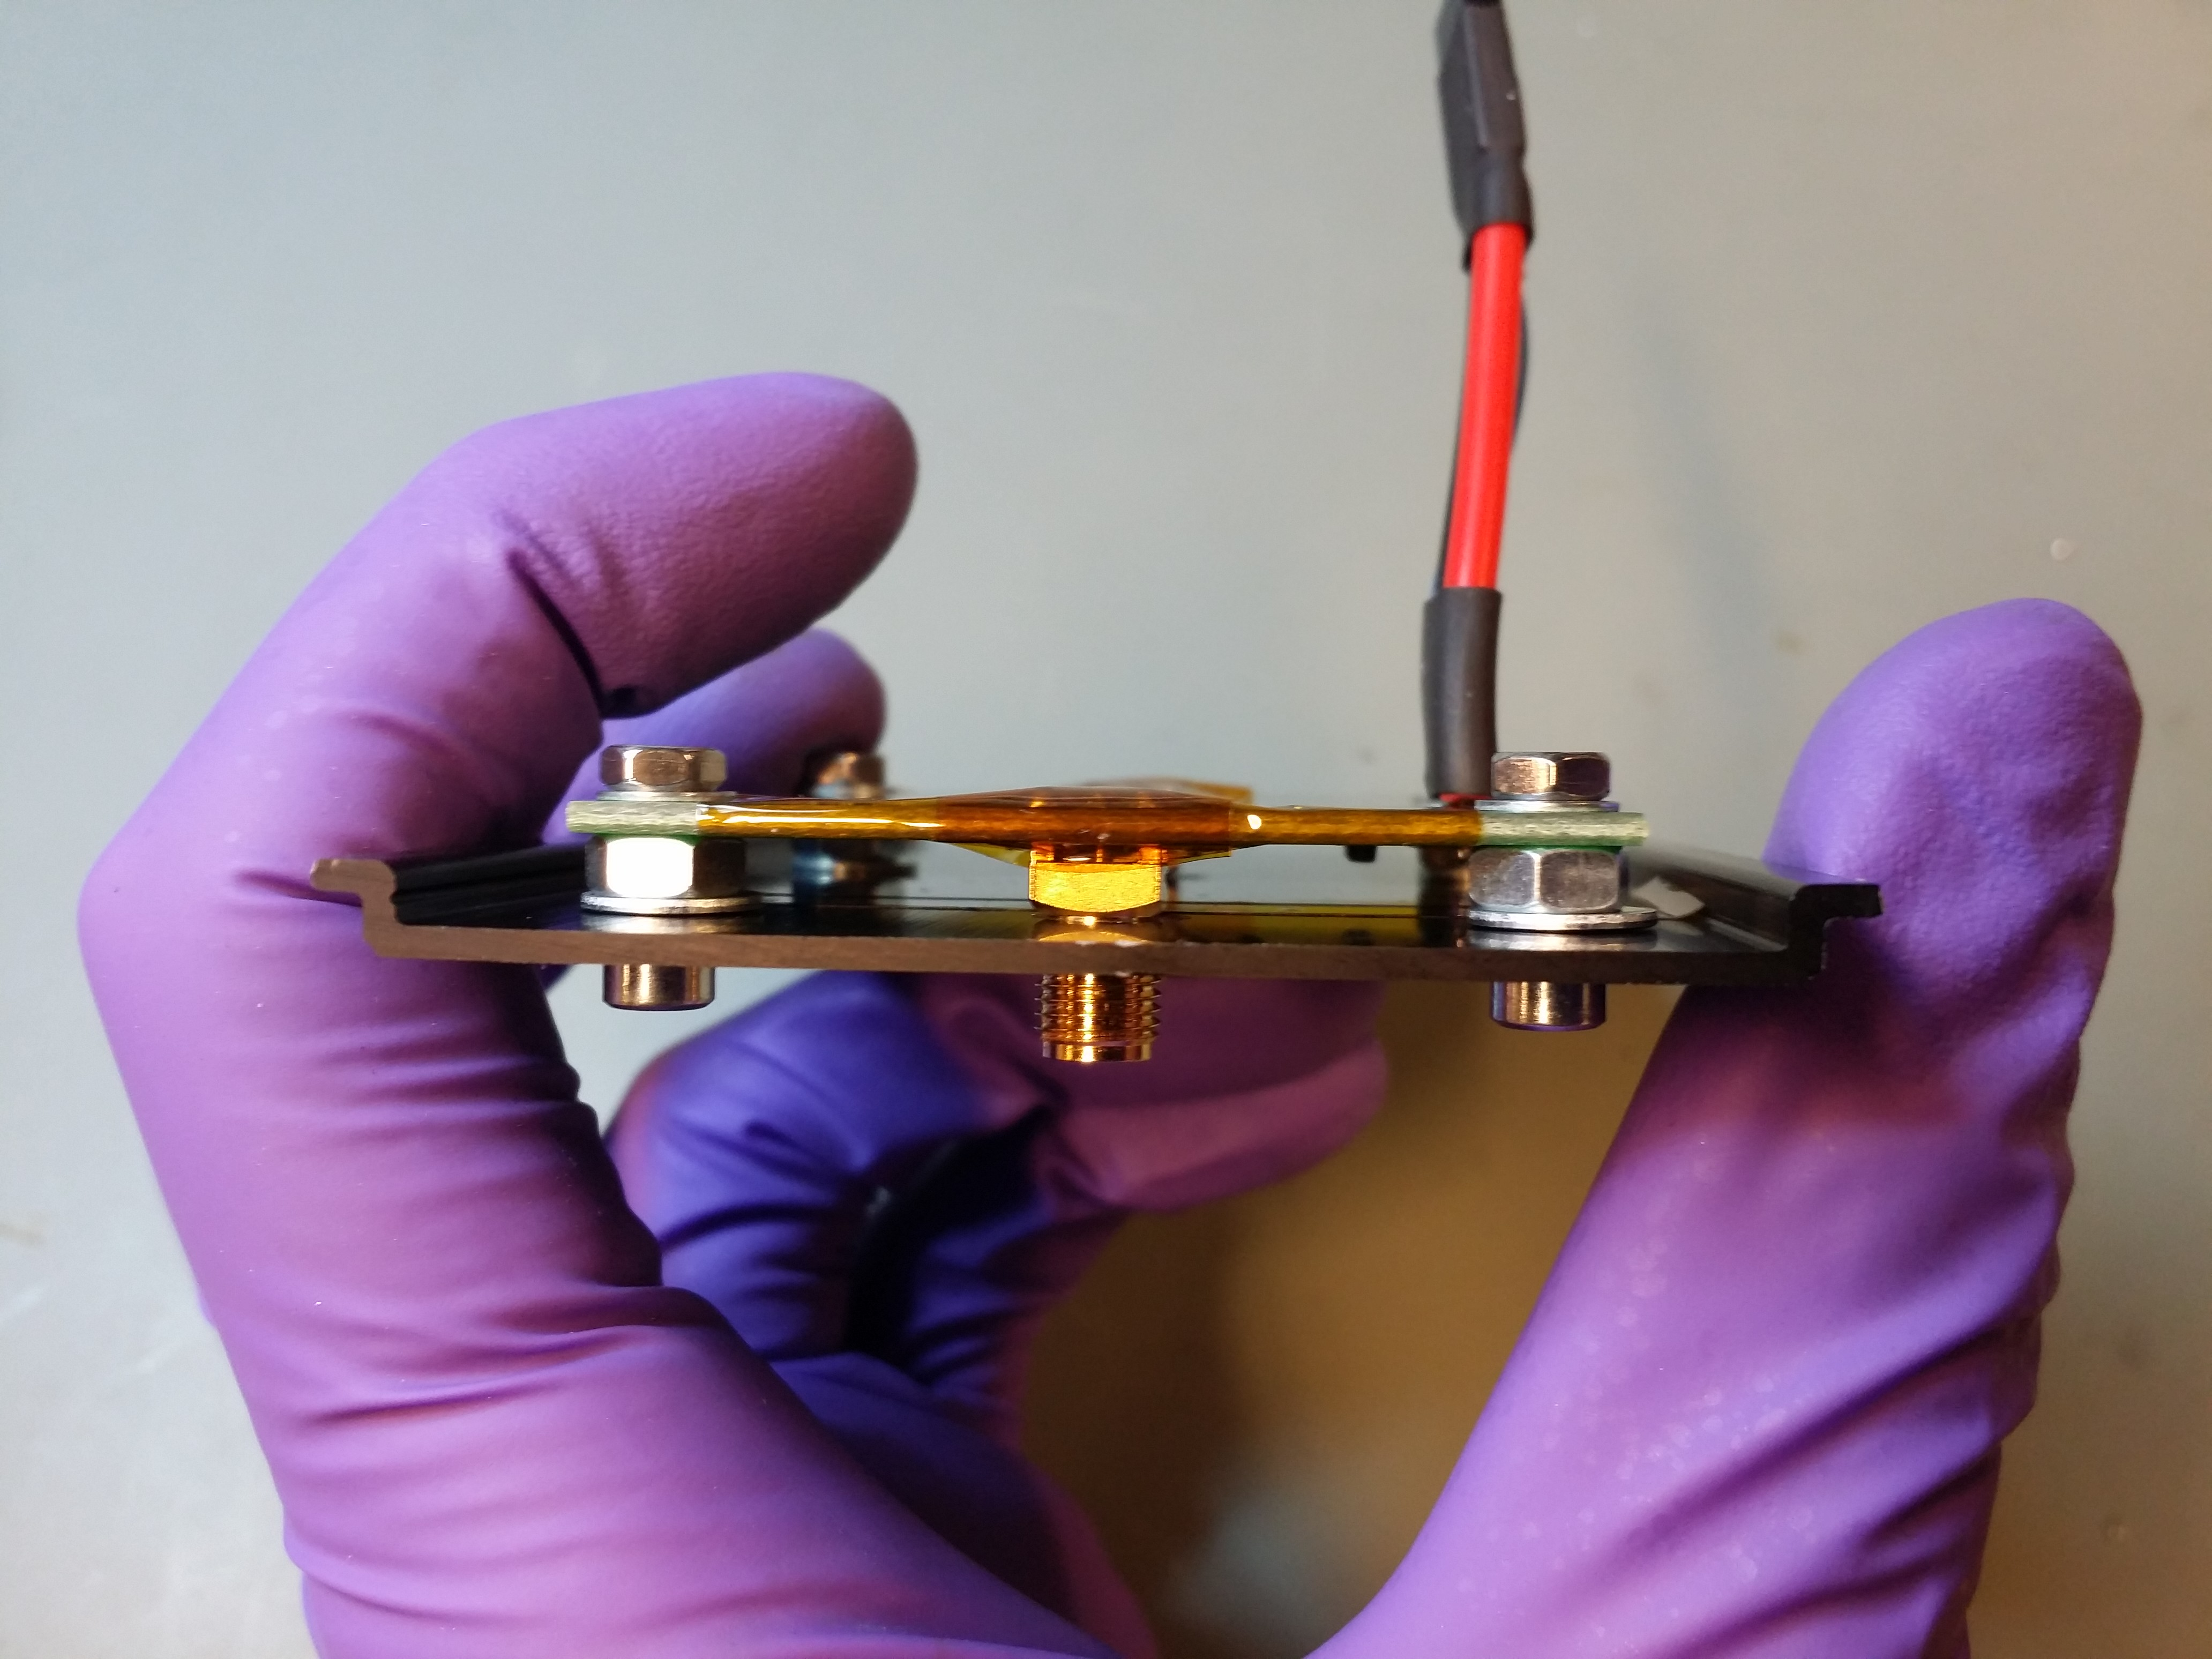
\includegraphics[width=\textwidth]{fig/IMG_20201201_121845.jpg}
\end{subfigure}

\begin{subfigure}[t]{0.48\textwidth}
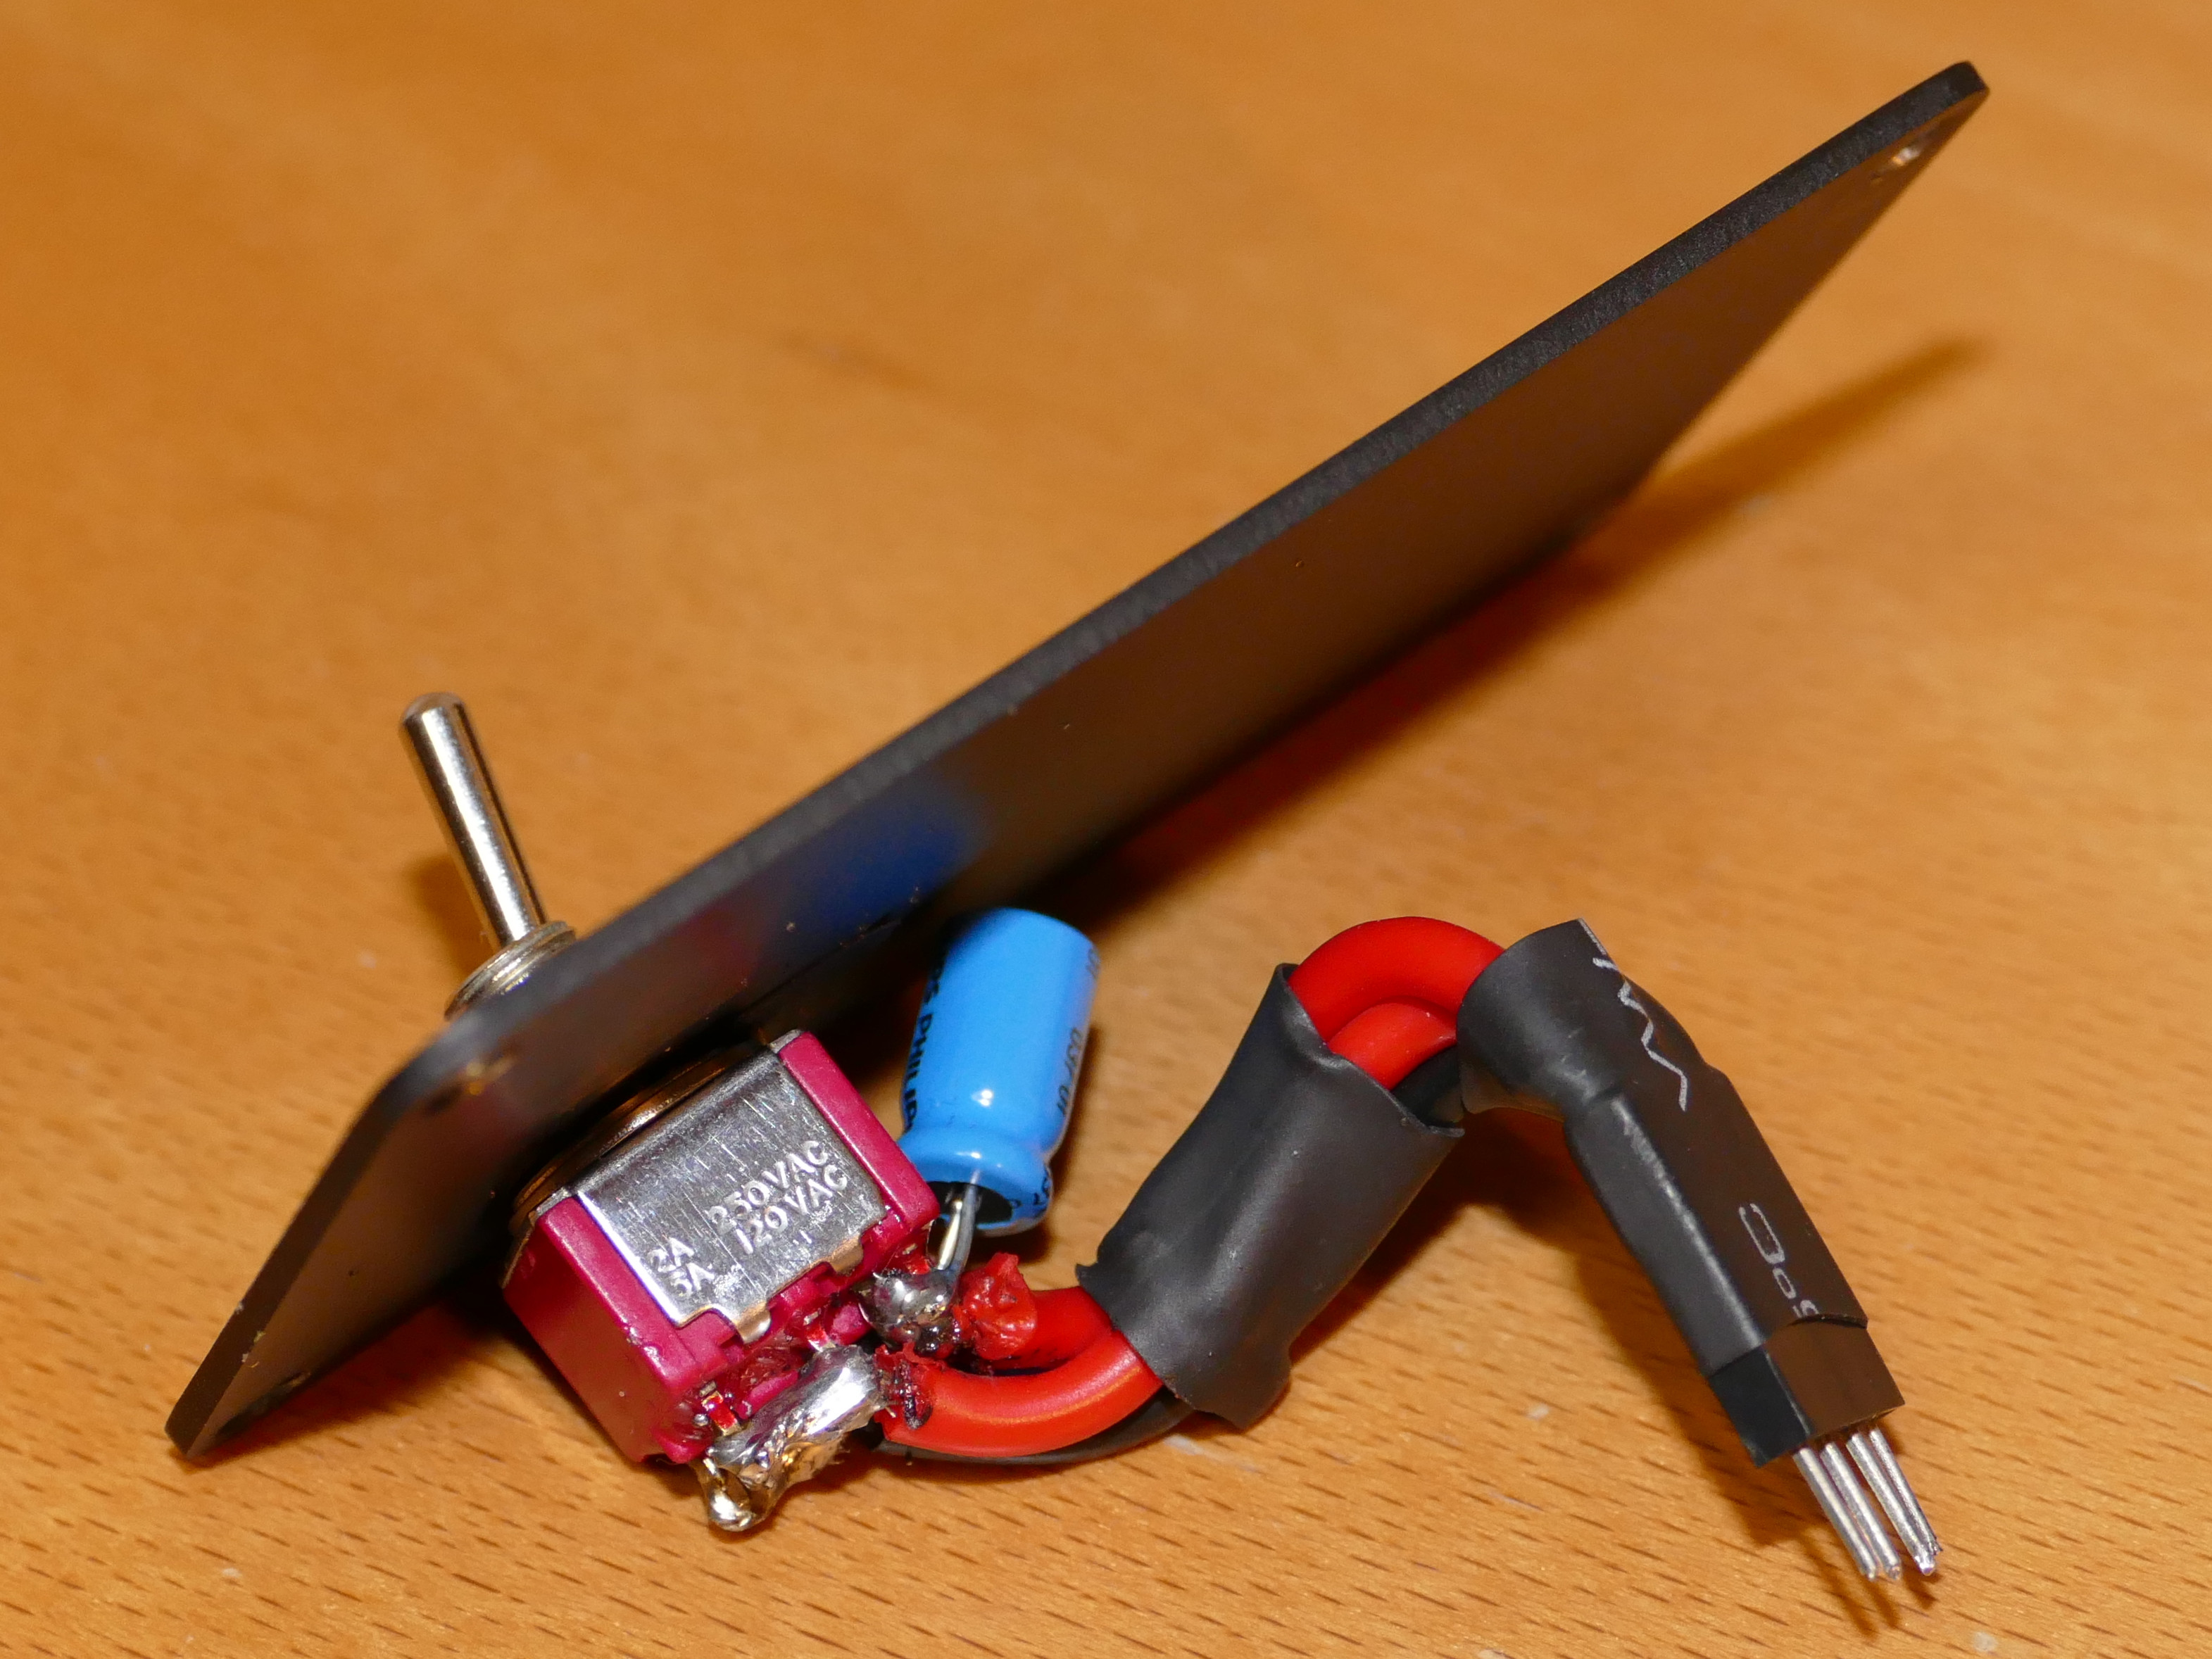
\includegraphics[width=\textwidth]{fig/P1170907-cropped.jpg}
\caption{Pre-amplifier switch panel}
\label{fig:pre_amp_switch}
\end{subfigure}
%
\begin{subfigure}[t]{0.48\textwidth}
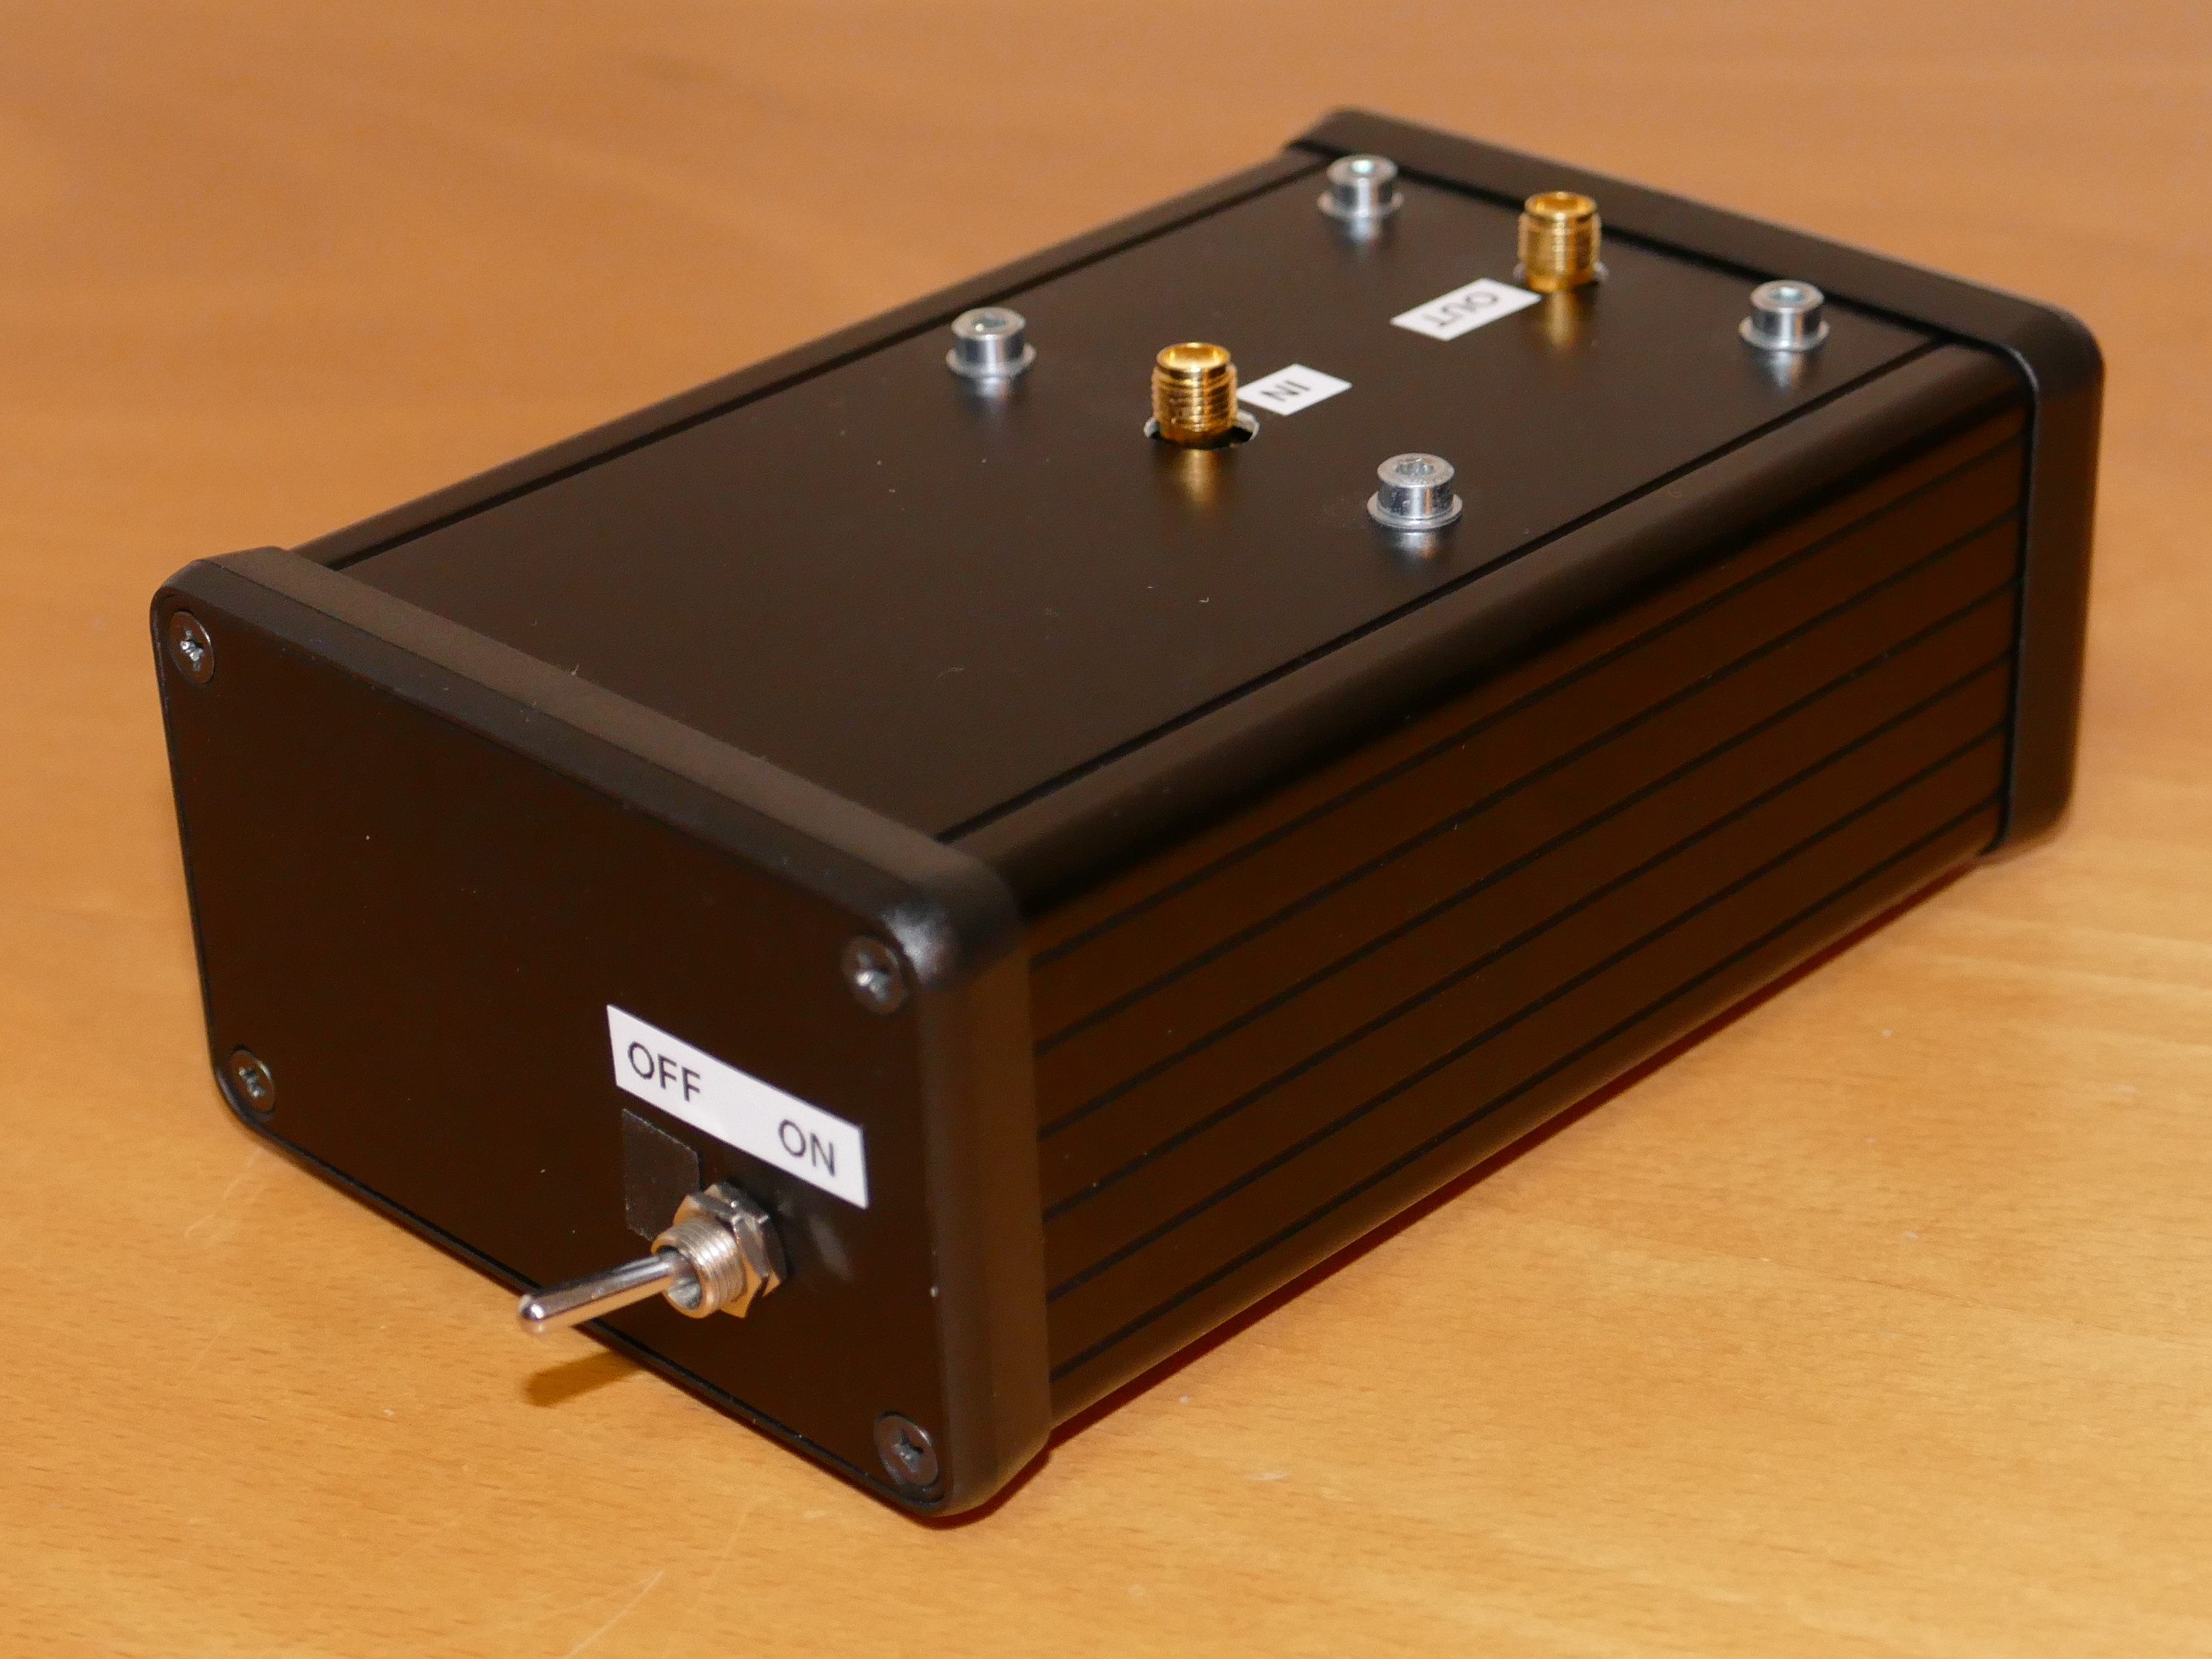
\includegraphics[width=\textwidth]{fig/P1170874-cropped.jpg}
\caption{Pre-amplifier}
\label{fig:pre_amp}
\end{subfigure}
%
\caption{Pre-amplifier case and mounting}
\label{fig:pre_amp_mounting}
\end{figure}


\FloatBarrier
Once the pre-amplifier was assembled, its frequency response was tested with an external pulser.
These results are plotted in figure \ref{fig:pre_amp_freq_response} with a cubic interpolation.
The frequency reponse is flat up to 10 kHz, but then fluctuates significantly, as the reflections of the signal within the amplifier become significant.

\begin{figure}[ht!]
\centering
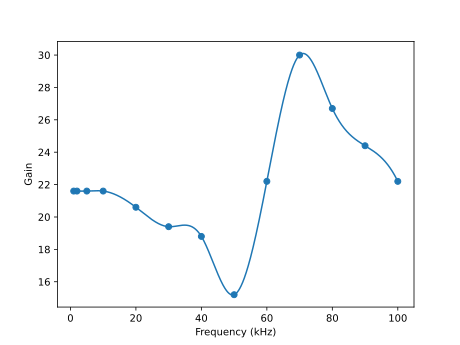
\includegraphics[width=\textwidth]{fig/python/preamp_freq_response}
\caption{Frequency response of the pre-amplifier}
\label{fig:pre_amp_freq_response}
\end{figure}

The dependence of the gain on the input amplitude was also tested.
For this an adjustable external attenuator was used, but it had to be calibrated first by measuring its attenuation as a function of the setting, which was an adjustable integer from 0 to 10.
This gave the results of figure \ref{fig:attenuator}.
We also established a linear fit to analyze the consistency of the results.
The pre-amplifier was then connected in series with the attenuator, and the calibration fit was used to obtain the attenuated input amplitudes.
The gain was then calculated as a ratio of the output and input amplitudes, and the results are plotted in figure \ref{fig:pre_amp_gain}.
Since no significant trend was detected in the results, we can estimate the gain to be the mean of the measured values: $G=21.51 \pm 0.44$.

\begin{figure}[ht!]
\centering
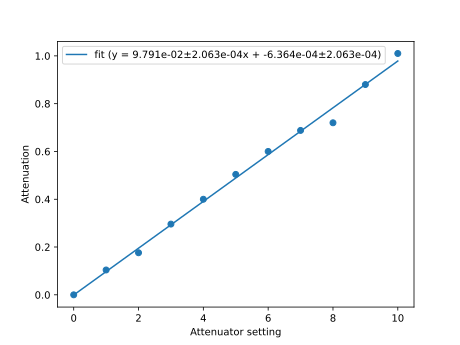
\includegraphics[width=\textwidth]{fig/python/attenuator}
\caption{Attenuator calibration at $f$ = 10 kHz}
\label{fig:attenuator}
\end{figure}

\begin{figure}[ht!]
\centering
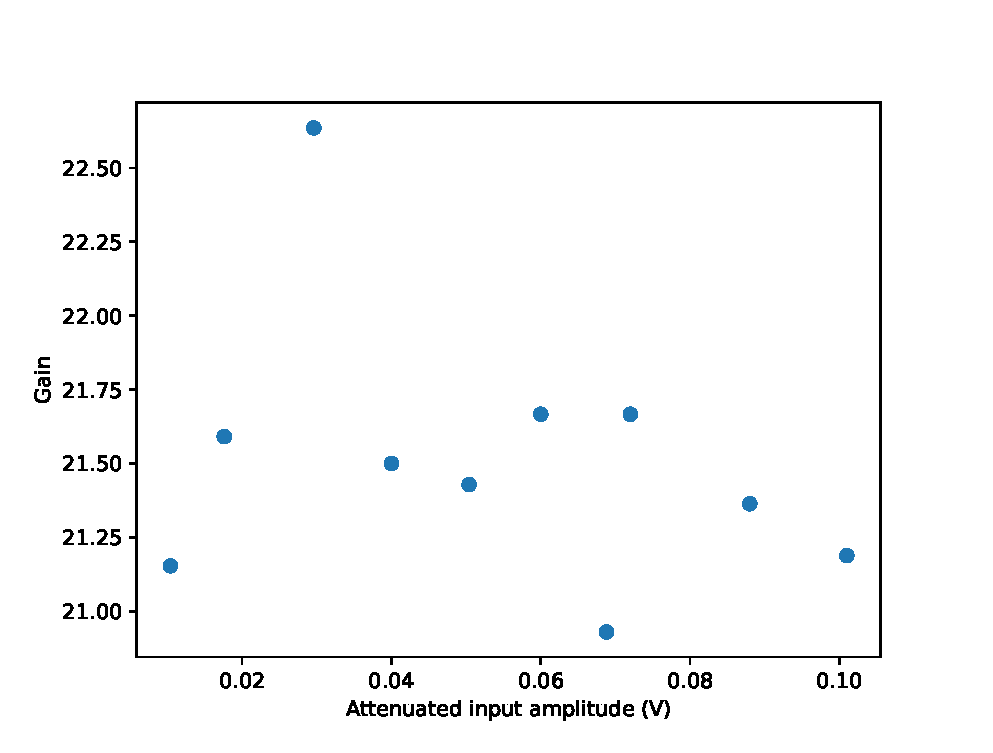
\includegraphics[width=\textwidth]{fig/python/preamp_gain}
\caption{Pre-amplifier gain by input amplitude at $f$ = 10 kHz}
\label{fig:pre_amp_gain}
\end{figure}

\FloatBarrier
Now that the gain of the pre-amplifier was known, it was installed to the setup to test its operation with the detector.
However, unfortunately the detector had degraded between the measurements with the commercial amplifier and these measurements, and we were not able to measure good spectra.
These failed results are plotted in \ref{fig:pre_amp_testing}.
However, the same pre-amplifier was also measured with the detector of a fellow student, and the results are plotted in figure \ref{fig:pre_amp_testing_nikita}.
The $^{55}$Fe spectrum and the primary peak of $^{241}$Am are clearly visible, but some of the secondary peaks of $^{241}$Am are lost in the noise.
In this measurement the amplification was also not ideal, as the $^{241}$Am peak is only around the channel 791, leaving some of the higher MCA channels unused.

\begin{figure}[ht!]
\centering
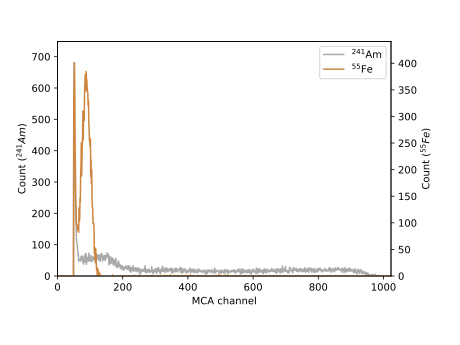
\includegraphics[width=\textwidth]{fig/python/spectra_custom_preamp}
\caption{Measured spectra with the custom pre-amplifier}
\label{fig:pre_amp_testing}
\end{figure}

\begin{figure}[ht!]
\centering
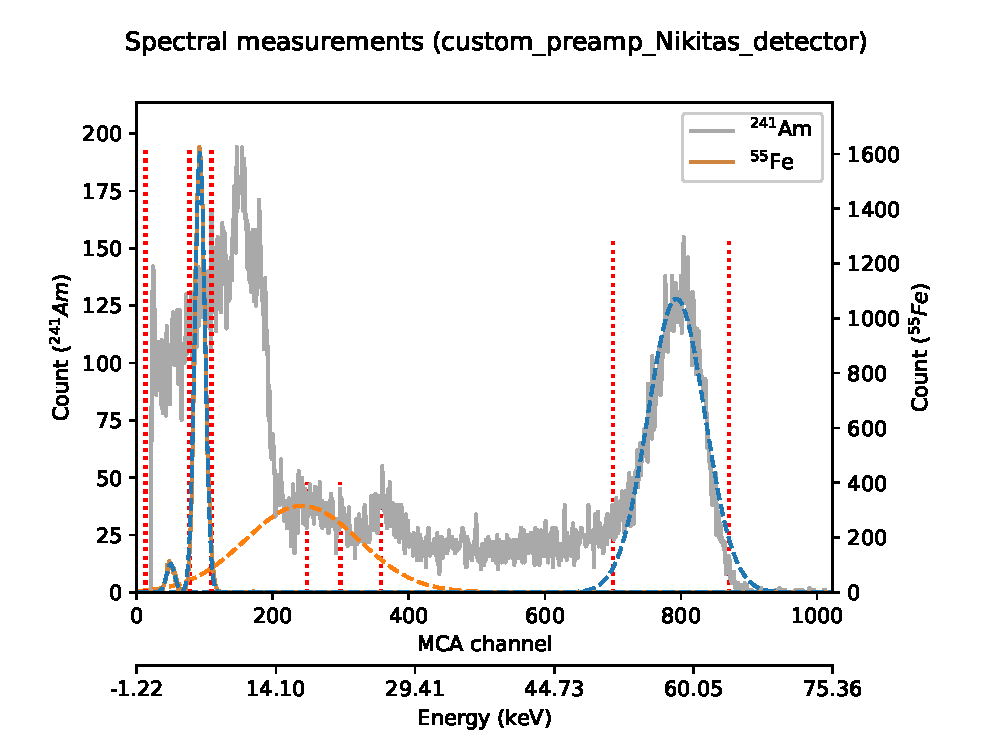
\includegraphics[width=\textwidth]{fig/python/spectra_custom_preamp_Nikitas_detector}
\caption{Measured spectra with the custom pre-amplifier and the detector of a fellow student}
\label{fig:pre_amp_testing_nikita}
\end{figure}


\FloatBarrier
Overall, despite the unexpected degradation of the detector, these results prove that the pre-amplifier is useful for its intended purpose with the measurement setup.
Its resolution is not as good as with the commercial amplifier, but it's highly cost-effective and compact, and has significant room for improvement.
For example, the gain could be made adjustable by replacing one of the resistors on the amplifier PCB with a potentiometer.
Additional improvements could also be made regarding the noise level, but on the other hand these can be worked around by increasing the measurement time.



\clearpage
\section{Pulser calibration}
\label{pulser_calibration}
It should be noted that the pulse heights measured with the oscilloscope differred significantly from those set on the pulser.
The relationship between these is illustrated in figure \ref{fig:pulser_calibration}.
The relative error of the pulser voltages was assumed to be 5 \% with a minimum error of 10 mV, and orthogonal distance regression was used for the fitting.

\begin{figure}[ht!]
\centering
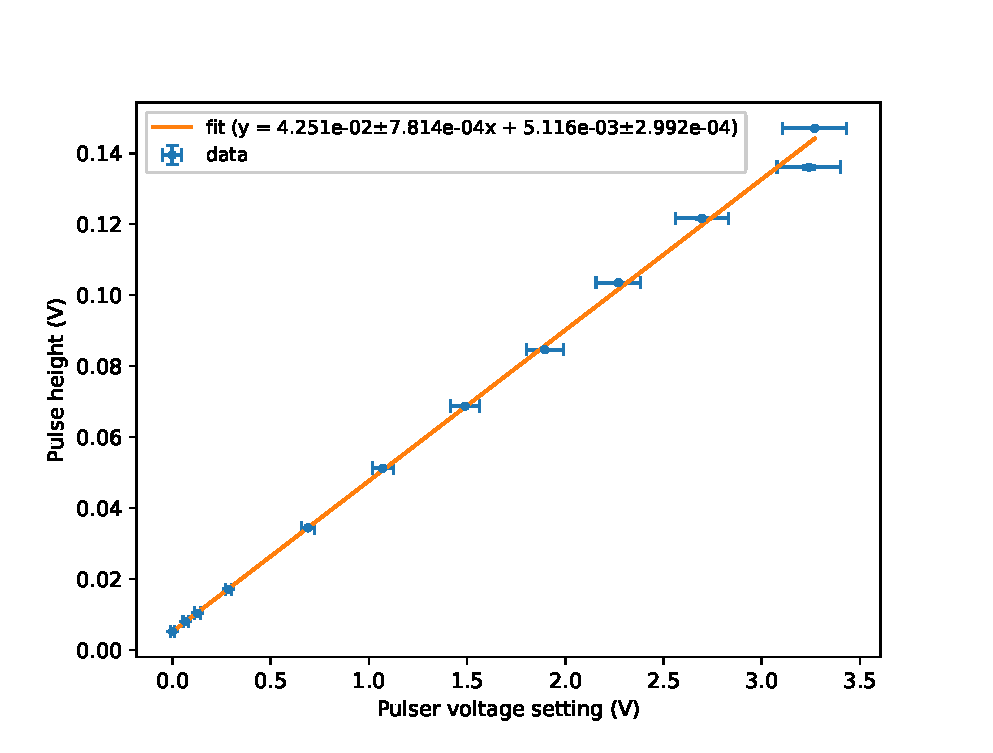
\includegraphics[width=\textwidth]{fig/python/pulser_calibration.eps}
\caption{Pulser calibration}
\label{fig:pulser_calibration}
\end{figure}



\clearpage
\section{Measurement data}
This appendix contains additional information on the measurement results.
The numerical values of the size measurements discussed in section \ref{assembly} are provided in table \ref{table:sizes}.

\begin{table}[ht!]
\centering
\caption{Size measurements
}
\begin{tabular}{l|l|l}
Measurement & $\mu$ & $\sigma$ \\
% \begin{tabularx}{\textwidth}{l|lllll|l|l}
% Measurement & \multicolumn{5}{l}{Data} & $\mu$ & $\sigma$ \\
\hline
Can outer diameter (mm)
% & 66.01 & 65.74 & 65.81 & 65.70 & 65.89
& 65.83 & 0.11 \\
Can top end inner diameter (mm)
% & 47.50 & 47.78 & 47.58 & 47.76 & 47.47
& 47.62 & 0.13 \\
Can top end outer diameter (mm)
% & 53.84 & 53.88 & 53.98 & 53.89 & 53.82
& 53.88 & 0.06 \\
Can bottom end inner diameter (mm)
% & 45.51 & 44.93 & 45.40 & 45.43 & 45.47
& 45.35 & 0.21 \\
Can thickness (\textmu m, from top section)
% & 240 & 250 & 240 & 250 & 280
& 252 & 15 \\
Can thickness (\textmu m, from cut can)
% & 102 & 103 & 102 & 100 & 102
& 101.8 & 1.0 \\
Long brass tube length (mm)
% & 29.25 & 29.26 & 29.27 & 29.27 & 29.25
& 29.26 & 0.09 \\
Short brass tube length (mm)
% & 10.05 & 9.98 & 9.99 & 9.99 & 10.04
& 10.02 & 0.03 \\
Brass tube diameter (µm)
% & 992 & 990 & 991 & 990 & 987
& 990.0 & 1.7 \\
Brass tube + connector length from acryl (mm)
% & 27.30 & 27.15 & 27.32 & 27.59 & 27.23
& 27.32 & 0.15 \\
Anode wire diameter (\textmu m)
& 49.0 & 2.0 \\
% \end{tabularx}
\end{tabular}
\label{table:sizes}
\end{table}


\section{Measurement notes}

This appendix contains copies of some of the original measurement note files.
The rest are formatted as large spreadsheets and could not therefore be included here.
However, all of the files are available in the GitHub repository.
\cite{repo}

\subsection{Environmental measurements}
\lstinputlisting{../analysis/data/notes/environment.txt}

\subsection{Gas leakage test}
\lstinputlisting{../analysis/data/notes/gas_leakage_test.txt}

\subsection{Size measurements}
{
% \UseRawInputEncoding
\lstinputlisting{../analysis/data/notes/size_measurements.txt}
}


\end{appendices}


\clearpage
\printbibliography


\end{document}